\chapter{Event reconstruction}\label{ch5}
The second step of the analysis, following the event selection, is the event reconstruction, where the $t\bar{t}$ final-state is rebuilt by the selected information from its decay products. Therefore, the reconstructed jets have to be assigned to the initial partons, taking the event topology and kinematics into account. For this reconstruction, the same approach as for the previous measurements~\cite{Aad:2015nba, ATLAS-CONF-2017-071} is used, based on a kinematic maximum likelihood fit. 

The details of the reconstruction are introduced in this section and the results, as well as the control distributions of the reconstructed observables are discussed.  


\section{Reconstruction of the $t\bar{t}$ final-state}
\begin{figure}[h]
	\centering
	\includegraphics[width=0.65\linewidth]{Pics/cp5/51}
	\caption{ Illustration of the reconstruction of the $t\bar{t}$ final-state. The  invariant masses of the hadronically and leptonically decaying top-quark are shown, as well as the corresponding $W$-boson masses. } 
	\label{fig:51}
\end{figure}

As displayed in~\cref{fig:51}, events with at least four jets are selected in this analysis. Therefore, one ends up with 4! = 24 possible jet-parton assignments, which will be denoted as permutations in the following. The minimum number of permutations gets further reduced by not distinguishing between the light jets of the $W$-boson decay, which results in a total of 12 permutations. 

In order to find the best jet-parton assignment, a kinematic likelihood fit is performed with the \textsc{KLFitter} framework~\cite{Erdmann:2013rxa}. Within this program, the best possible jet-parton matching is evaluated based on the leading-order kinematics of the $t\bar{t}$ decay. For each permutation of the jets, a kinematic likelihood function ($L_{ \textsc{KLFitter}}$) is defined, using reconstructed properties like the hadronic $W$-boson mass, which is the invariant mass of the two jets of the hadronic top-quark decay $m(q_1q_2)$. In the following, $q_1$ and $ q_2$ denote the light quarks of the $W$-boson decays, where $b_{\rm had}$  is referred to  the $b$-quark from the hadronic top-quark decay and $b_{\rm lep}$ to the leptonic one.  $E_{\rm jet_i}$ is the energy of the jet with number $i$. Properties of the charged lepton are labelled with $l$, while $\nu$ denotes the neutrino. All masses shown in~\cref{fig:51} are calculated and related to the  predicted kinematics for the leptons and the quarks of the $t\bar{t}$ decay.


The input variables for the kinematic likelihood fit are the four momenta of the charged lepton $E_{\rm l_i}$, the $y$ and $x$ components of the missing transverse momentum ($p_{\nu,x}$, $p_{\nu,y})$ and the four momenta of the jets. For events with at least two $b$-jets, the two highest $p_T$ $b$-tagged jets and the two untagged jets, with the highest $p_T$,  are used.
If the event contains more than four jets, the reconstruction efficiency can be increased by allowing more jets as input to  \textsc{KLFitter}. As shown in~\cite{ATLAS-CONF-2017-071}, using up to six jets is beneficial for the event reconstruction. Furthermore, the so-called veto mode is applied to improve the reconstruction efficiency and to reduce the number of possible permutations. This mode does not allow to assign a $b$-jet as a light jet and vice versa. 

The kinematic likelihood function is given by eq.~(\ref{eq:Likeklf}) and consists of products of Breit-Wigner distributions ($BW$) and transfer functions ($T$).
The $BW$ distributions are based on a leading-order picture where all jets are matched with the corresponding partons and  the pole masses of the top-quarks~\cite{Erdmann:2013rxa}. 
Therefore, the $BW$ distributions are calculated for the input momenta of the quarks and leptons with the corresponding invariant masses and the transverse momentum of the neutrino. The first expression in the $BW$ terms correspond to the different invariant masses of the system and represent the abscissa of the distribution. The used invariant masses are the two jet mass of the light jets ($m(q_1q_2)$) , the  mass of the lepton pair ($m(l \nu)$), the mass of the hadronically decaying top quark ($m(q_1q_2 b_{\rm had})$) and the mass of the leptonically decaying top quark ($m(q_1q_2 b_{\rm lep})$).
A straight line in the $BW$ brackets separates the variables from the parameters which determine the functional form of the distributions. These parameters are the location parameter of the distribution, where the mass of the $W$-boson and of the top quark are considered, as well as the corresponding shape parameter (width) of the distribution, which are denoted with $\Gamma$. Here, the mass parameter of the $W$-boson is set to the official particle data group  result of 80.39 $\pm$ 0.015~GeV~\cite{Olive:2016xmw}. The top-quark mass  is determined as a free parameter by the kinematic likelihood fit and therefore called reconstructed top-quark mass $m_{\text{top}}^{\rm reco}$.

\begin{eqnarray}
\label{eq:Likeklf}
L_{\textsc{KLFitter}} &=& 
BW[m(q_1q_2)|m_{\rm W},\Gamma_{\rm W}]\cdot BW[m(l \nu)|m_{\rm W},\Gamma_{\rm W}]\cdot\ \nonumber\\
&&BW[m(q_1q_2 b_{\rm had})| m_{\text{top}}^{\rm reco},\Gamma_{\rm top}]\cdot BW[m(l \nu b_{ \rm lep})|m_{\text{top}}^{\rm reco},\Gamma_{\rm top}]\cdot \nonumber \\
&&T(E_{\rm jet_1}|\hat{E}_{b_{\rm had}})\cdot T(E_{\rm jet_2}|\hat{E}_{b_{\rm lep}})\cdot \nonumber \\ 
&&T(E_{\rm jet_3}|\hat{E}_{q_1})\cdot T(E_{\rm jet_4}|\hat{E}_{q_2})\cdot \nonumber \\
&&T(E_{x}^{\rm miss}|\hat{p}_{x,\nu})\cdot T(E_{y}^{ \rm miss}|\hat{p}_{y,\nu})\cdot \nonumber\\ &&T(E_{y}^{\rm miss}|\hat{p}_{y,\nu}) \cdot 
\left\{\begin{array}{II}
T(E_{e}|\hat{E_e}) \hspace{0.5cm} \text{ $e$ + jets}\\

T(p_{T_{\mu}}|\hat{p}_{T_{\mu}}) \hspace{0.5cm} \text{ $\mu$ + jets}\\
\end{array}
\right\} \cdot W_{\rm btag}\phantom{L =aaaaaaaa } 
\end{eqnarray}



The transfer functions represent the detector response and further disturbances, by describing the resolution of the reconstructed energies. Therefore,  the jet energies $E_{\rm jet_i}$ ($i$ = 1,2,3,4)  are taken into account. In the likelihood expressions, like $T(E_{\rm jet_1}|\hat{E}_{b_{\rm had}})$, the fist term in the brackets represent the variable of the transfer function, while the second expression denotes the energy or the transverse momentum of the associated physical patron-level quantity (denoted by a hat), which are taken into account as additional information. Furthermore, there are transfer functions, which include the missing transvers energy by using  the corresponding components of the transverse momentum, e.g. $T(E_{x}^{\rm miss}|\hat{p}_{x,\nu})$. As shown in e.q.~(\ref{eq:Likeklf}), different functions for muon and electron events are used. While for electrons the energy is taken into account for, muons the transverse momentum is considered.

 Due to the changes, which arise with the increasing center-of-mass energy, e.g. the different background evolution in $\sqrt{s}$, the transfer functions have to be obtained specifically for the conditions of the measurement. However, within the time scale of this thesis, the corresponding transfer functions for $\sqrt{s}=$13~TeV were not available. Therefore, the same transfer functions as for the 8~TeV measurement are used~\cite{ATLAS-CONF-2017-071}. The  transfer functions have a double Gaussian from and are parametrized with the five parameters ($p_i$):
\begin{equation}\label{transfer}
T(\Delta E) = \frac{1}{\sqrt{2\pi}(p_2 + p_3p_5)}
\begin{pmatrix}
e^{\frac{(\Delta E- p_1)^2}{2p_2^2}} + p_3e^{\frac{(\Delta E- p_4)^2}{2p_5^2}} 
\end{pmatrix}
\end{equation} 
The motivation for the double Gaussian is  the energy resolution of the detector, which can be described by the displayed functional form. 
It describes the spectrum of the relative difference of the parton-level energy $E_{\rm Truth}$ and the reconstructed energy $E_{\rm reco}$:
\begin{equation}
\Delta E = \frac{E_{\rm Truth}-E_{\rm reco}}{E_{\rm Truth}}.
\end{equation}
The last term of the likelihood is a $b$-tagging weighting factor $W_{\rm btag}$ is applied, which is 1 if the $b$-tagged jets and the untagged jets are in the correct position, and 0 otherwise. 







%%%%%%%%%%%%%%%%%%%%%%%%%%%%%%%%%%%%%%%%%%%%%%%%%%%%%%%%%%%%%%%%%%%%%%%%%%%%%%%%%%%%%%%%%%%%%%%%%%%%%%%%%%%%%%%%%%%%%%%


\subsection{Analysis specific quantities}

This analysis is based on the template methode (see~\cref{Relevanz}), which is a common analysis technique in high energy physics. Due to the nature of the uncertainties which affect the measurement of the top-quark mass is determined together with two scale factors, which are sensitive to the energy calibration of the jets.  
These are the so-called jet energy scale factor (JSF) and the  $b$-to-light jet energy scale factor (bJSF). A detailed definition of the two scale factors, as well as of the motivation for the multidimensional template fit is given in~\cref{sec:Temp1}.
Three estimators have been introduced, which provide the sensitive to top-quark mass and the energy scale factors. In this subsection, these estimators are introduced, since they are based on the event reconstruction.

 The first estimator is the reconstructed top-quark mass $m_{\text{top}}^{\rm reco}$, which  is a free parameter in \textsc{KLFitter} and takes the implicit constraint in the fit to the known $W$-boson mass into account. It is sensitive to the top-quark mass and both scale factors.
 Secondly, there  is the reconstructed $W$-boson mass ($m_\text{W}^{\rm reco}$), which is the invariant mass of the hadronically decaying top-quark. While $m_{\text{top}}^{\rm reco}$ is determined by the kinematic likelihood fit, $m_\text{W}^{\rm reco}$ is calculated from the original four vectors of the chosen jet permutation and is sensitive to the JSF.
 A third estimator  ($R_{\text{bq}}^{\rm reco}$) is introduced to provide the sensitivity to the bJSF and its definition depends on the number of $b$-tagged jets. Nevertheless, both definitions are calculated, as $m_\text{W}^{\rm reco}$, from the original four vectors of the chosen jet permutation. 
  If only one $b$-tagged jet is required, $R_{\text{bq}}^{\rm reco}$ is defined via the transverse momentum of the $b$-tagged jet divided by the averaged scalar sum of the transverse momenta of the two untagged jets which are associated to the hadronic $W$-boson decay (see~\cref{rbq}).
 For events with two $b$-tagged jets, $R_{\text{bq}}^{\rm reco}$ is defined as the ratio of the scalar sum of the transverse momenta of the $b$-tagged jet of the leptonic decaying top quark and the $b$-tagged jet of the hadronic decaying top quark and the scalar sum of the transverse momenta of the two untagged jets from the hadronic $W$-boson decay (see~\cref{rbq2}).

\begin{equation}\label{rbq}
R^{\rm reco,1b}_{\rm bq} = \frac{2 p_T^{\rm b_{\rm tag}}}{(p_T^{\rm W_{\rm jet_1}}+p_T^{\rm W_{\rm jet_2}})}
\hspace{0.5cm}
\text{and}
\end{equation}
\begin{equation}\label{rbq2}
R^{\rm reco,2b}_{\text{bq}} = \frac{p_T^{\rm b_{\rm had}}+ p_T^{\rm b_{\rm lep}}}{(p_T^{\rm W_{\rm jet_1}}+p_T^{\rm W_{\rm jet_2}})}.
\end{equation}
In terms of this analysis, only events with at least two $b$-jets are used for the reconstruction. Thus, only the second definition for  $R_{\text{bq}}^{\rm reco,2b}$ is used here and just called $R_{\text{bq}}^{\rm reco}$ in the following. 

Furthermore, all three reconstructed variables are constrained by cuts, which are implemented before the event reconstruction:  $m_{\text{top}}^{\rm reco}  \subseteq [125,200]$~GeV,  $m_{\text{W}}^{\rm reco}  \subseteq [55,110]$~GeV and $R_{\text{bq}}^{\rm reco}  \subseteq [0.3,3.0]$. Moreover, events where the minimization of  \textsc{KLFitter} does not converge, are rejected. These cuts are applied on top of the cuts of the preselection.





\subsection{Event yields}

In~\cref{tab:T41} the event yields, obtained with the above introduced selection criteria are shown for events with at least four jets, where at least two of the jets have to be tagged as $b$-jets. The total number of data events is shown, as well as the corresponding signal and background contributions. Furthermore, the event yields for events with four jets and at least one $b$-tagged jet, are displayed. 
For the data-simulation comparison the top-quark mass is assumed to be 172.5~GeV. If not mentioned otherwise, all results just include statistical uncertainties. There are no uncertainties assumed for displayed values of the data. 

\vspace{0.5cm}
\begin{center}\
\captionof{table}{The observed number of events for a center-of-mass energy of 13~TeV and an integrated luminosity of 33~fb$^{-1}$. The event yields are presented for events with at laest four jets with at least two $b$-tagged jets. Furthermore, the number of signal and background events for the nominal sample of $m_{\rm top} =$ 172.5~GeV are shown. The simulated results correspond to the  luminosity of the data. The statitical uncertaities are rounded to two significant digits.}\label{tab:T41}


	
\vspace{0.3cm}	
	

\begin{tabular}{>{}m{4.0cm}>{}m{3.0cm} >{}m{3.0cm}} \toprule

Process (Simulation)&   2 $b$-tags&  1 $b$-tags\\
\midrule
$t\bar{t}$ & 389550 $\pm$ 390& 720620$\pm$  520\\
Single top & 12909 $\pm$  66&36070 $\pm$  110\\
$W$+jets & 8000 $\pm$  410&79510 $\pm$  990\\
$Z$+jets & 1810 $\pm$  90&13300 $\pm$  260\\
Diboson & 387.5 $\pm$  8.7&2957 $\pm$  28\\
$t\bar{t}+V$ & 18.17$\pm$  0.31&27.72 $\pm$  0.39\\
\midrule
Total signal + background & 412670 $\pm$  580&852500 $\pm$  1200\\
\midrule
Data & 475166 &  998651\\
\midrule
Data/Prediction  &1.15 $\pm$ 0.0016 & 1.17 $\pm$ 0.0016\\

\bottomrule
\end{tabular}

\end{center}












\vspace{1.0cm}

In~\cref{tab:T41}, the shown single top events are treated as an additional background process.
The main background stems from $W$ + jets events. For the sample with at least two $b$-tags it is  2~\% of the total background and for the sample with one $b$-tag it is 9~\%. However, the QCD-multijet background has not be estimated yet and might lead to noticeable contributions for the future analysis. The other background sources, e.g.  diboson  and $Z$ + jet events, play only a minor role. 
The choice of the selection cuts on events with at least two $b$-tagged jets, can be explained by the nature of the top-quark pair decay, which almost always produces two $b$-quarks.  As shown here, as well as by the previous measurements, the main background sources can be reduced impressively by the cuts on the number of tagged jets. In case of this analysis, the total background gets reduced from  15~\% to 6~\% for events with two  $b$-tags. While this remarkable reduction leads to a noticeable decrease of the background, the predicted number of events remain consistent with the observed number in data. Based on this experiences, the selection cuts on events with at least four jets, where at least two have to be tagged as $b$-jets are used for this analysis.

Despite the fact that the three measurements at 7, 8 and 13~TeV are sharing the same main background sources, the relative contributions are different for each center-of-mass energy. This can be explained by the fact that the cross-sections of the different backgrounds depend differently on the increasing center-of-mass energy.


\subsubsection{Global quantities of the preselection}

In~\cref{fig:Sel1,fig:Sel2,fig:Sel4}, chosen distributions of observables are displayed for events with at least two $b$-tagged jets, together with the data-simulation comparison ratio. These control plots correspond to the  2016 ATLAS data set, obtained at 13~TeV with a corresponding integrated luminosity of 33~fb$^{-1}$. The different backgrounds are also shown by the coloured histograms. 

If not mentioned otherwise, all shown distributions contain only statistical uncertainties and the  predicted distributions are normalised to the observed number of events in data, due to the sensitivity of the top-quark mass on the distribution shape~\cite{ATLAS-CONF-2017-071}. For the generation of  the control distributions, the \textsc{Powheg} + \textsc{Pythia 6} samples are used.

In general more events in data than in simulation can be seen, which seems to be consistent for all observables. Furthermore a slight offset, of the data points to the simulation can be observed in the normalization of several distributions.    
Here one as to keep in mind, that the QCD background is missing, as well as the systematic uncertainties.

%Nevertheless, one has to mention, that there is one deviation from the good trend in the data-simulation comparison. For the third bin of the number of tagged jets~\cref{fig:Sec2} a  disagreement can be seen. This issue has already been noticed by previous analyses and is assumed not to affect this measurement.

The displayed control distributions test also the quality of the Monte Carlo simulation.
Disagreements in the data-prediction comparison can for example  arise due to imperfections in the  modelling  with different physics generators. Furthermore, disagreements can appear if the \textsc{Geant4} simulation of the detector is not good enough. Therefore, the improvement of the simulation is one of the key tasks for the general physics analysis. 
The control distributions for the reconstructed quantities, are shown after the global quantities of the preselection.



\begin{figure} [b]% "[t!]" placement specifier just for this example
	\centering
\begin{subfigure}{0.25\textwidth}
	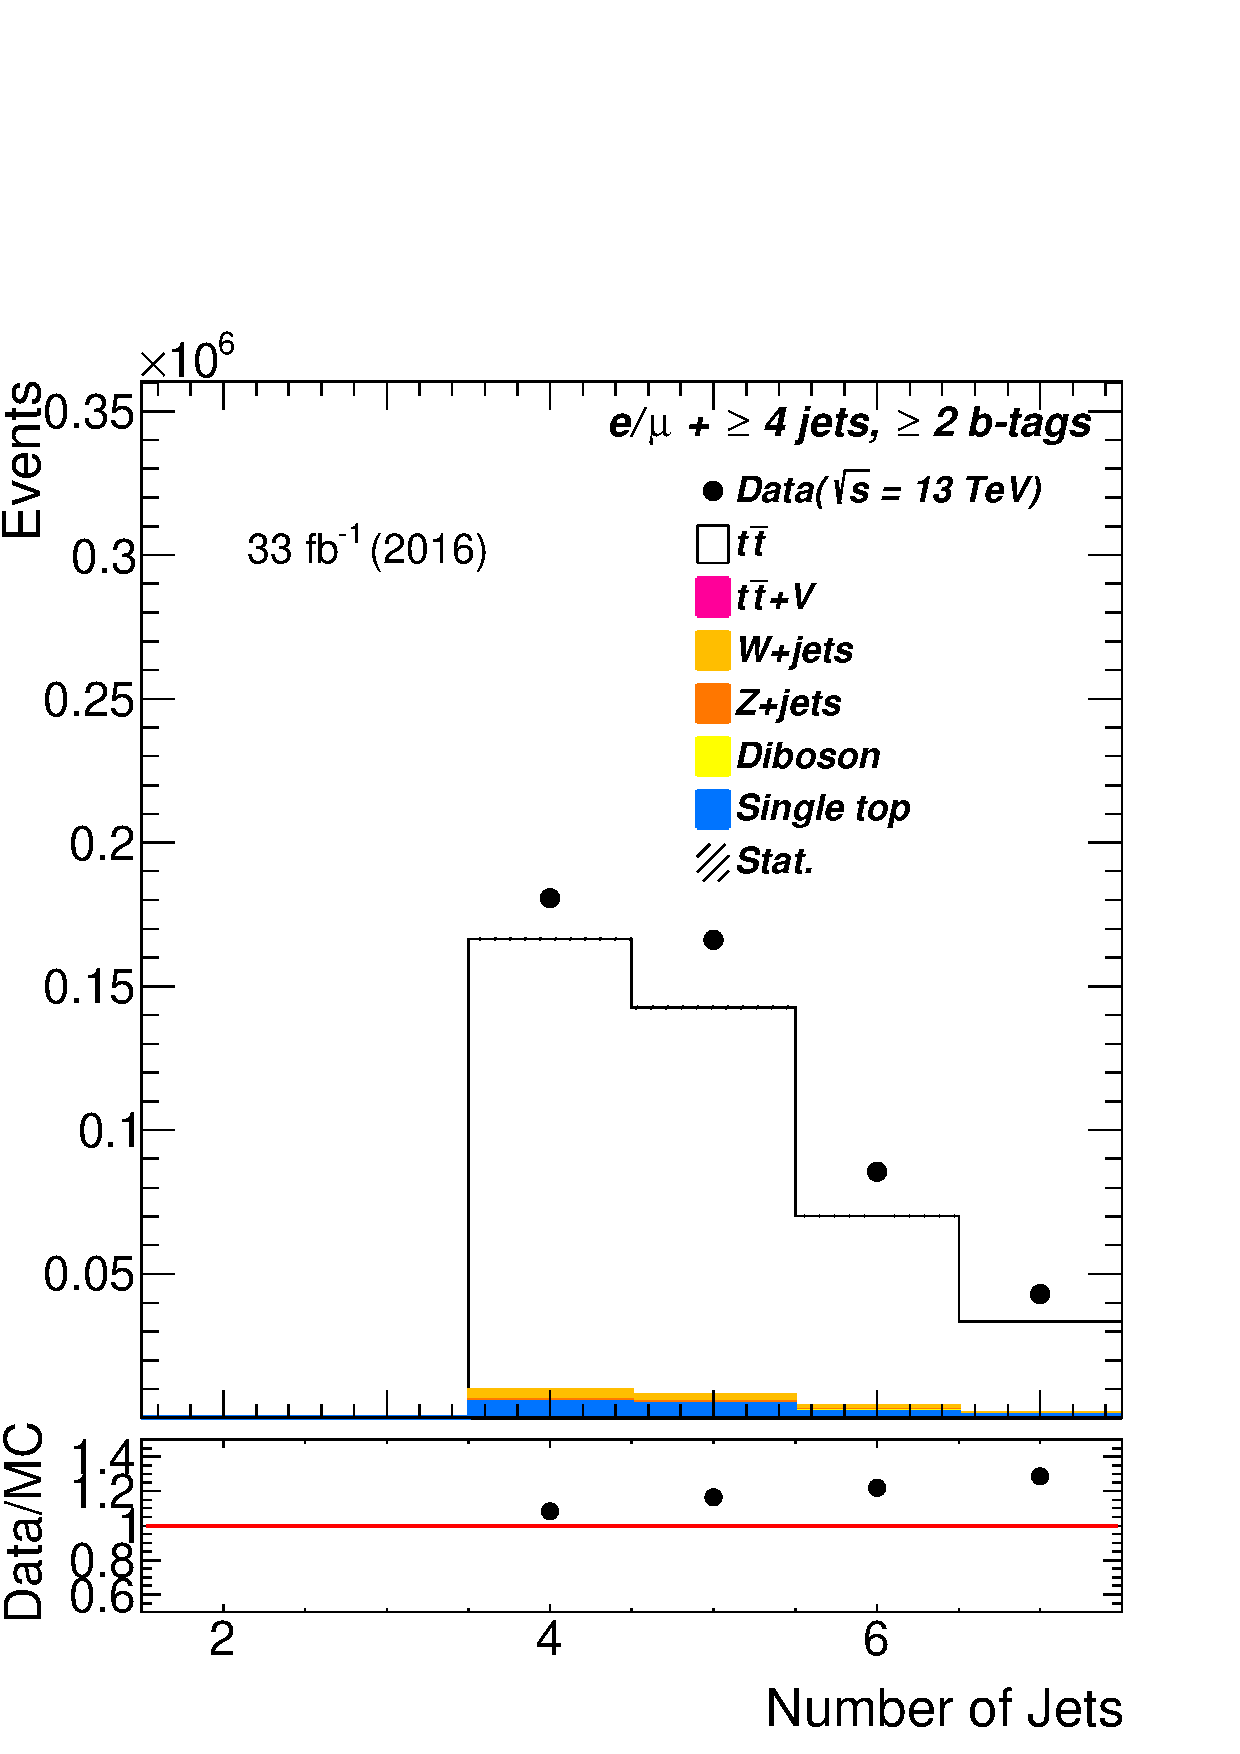
\includegraphics[width=\linewidth]{ControlPlots_emujets_2016_4incl_2incl/jet_n_emujets_2016.png}
	\caption{Number of jets.} \label{fig:Sec1}
\end{subfigure}
\hspace*{0.5cm}
\begin{subfigure}{0.25\textwidth}
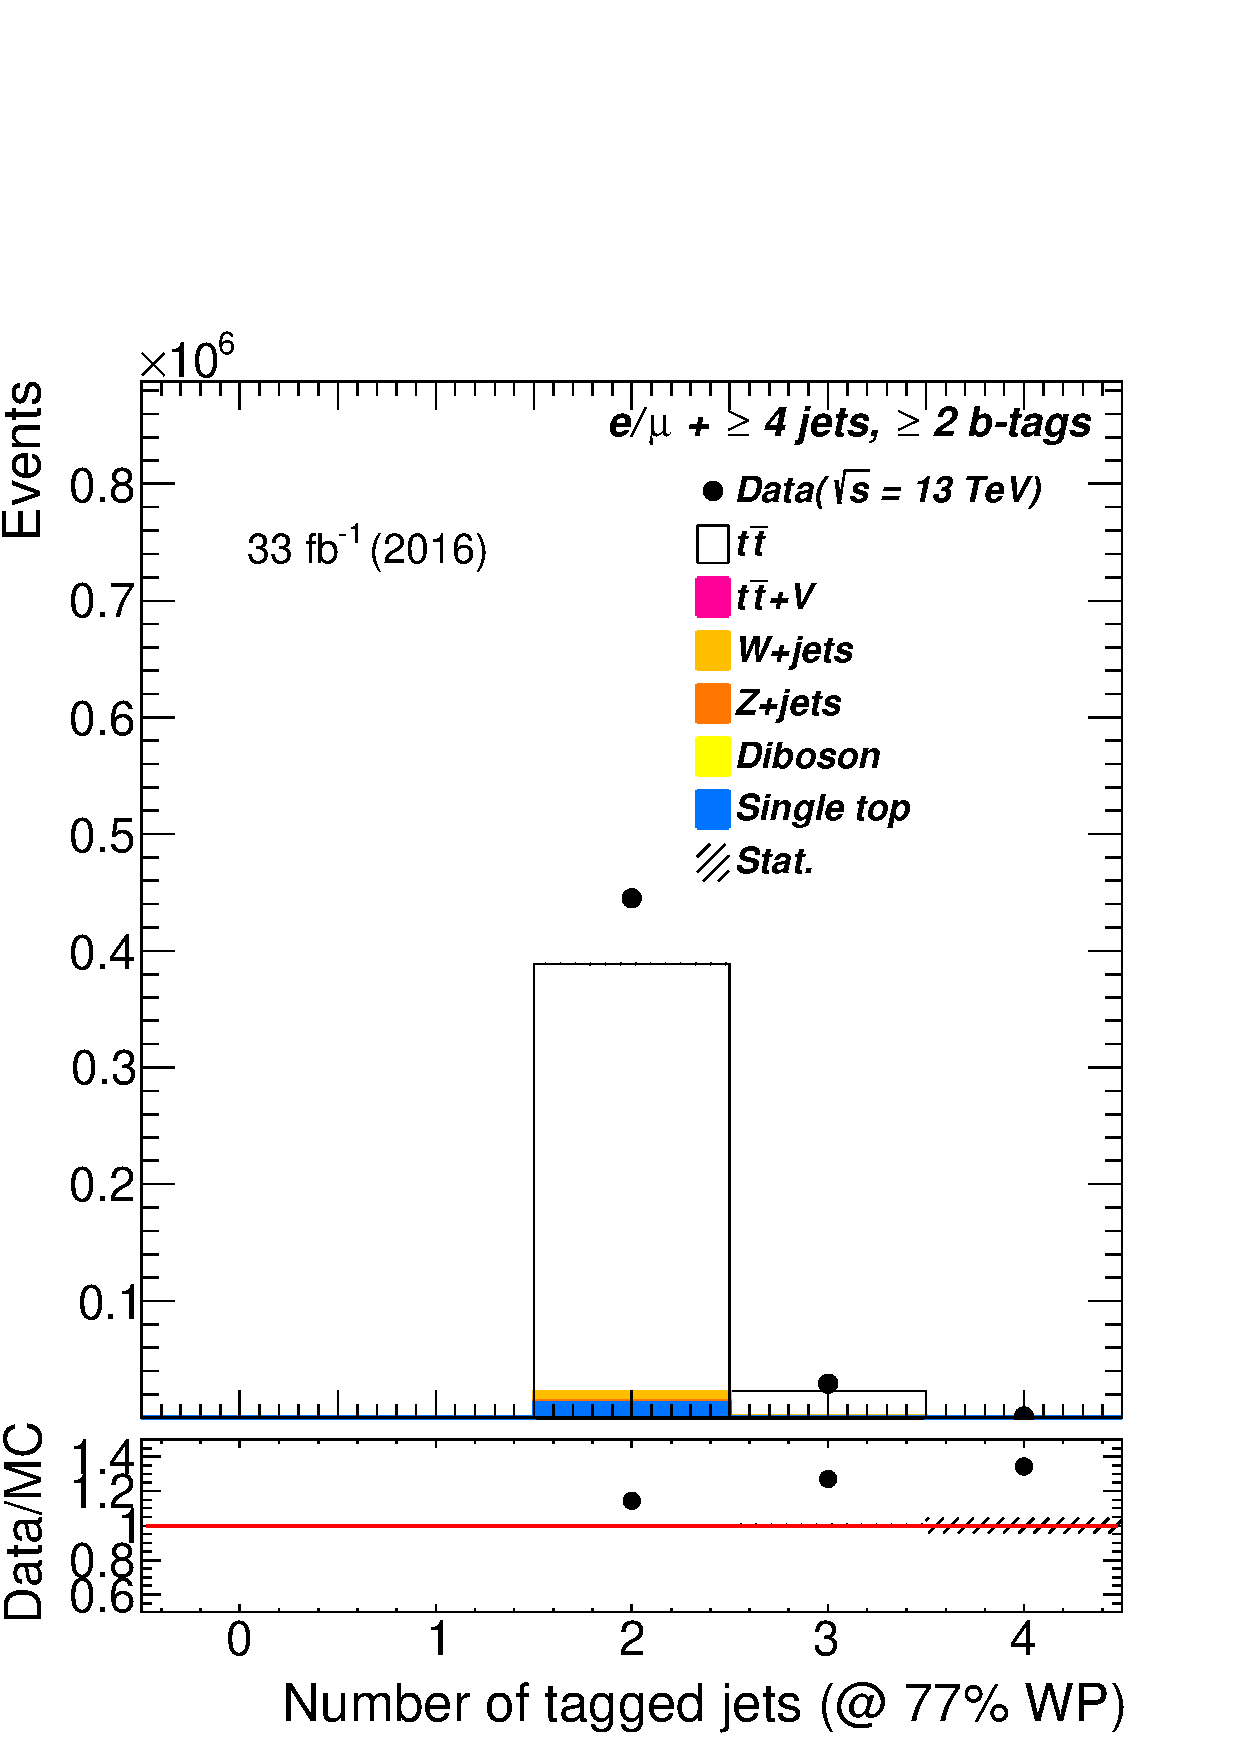
\includegraphics[width=\linewidth]{ControlPlots_emujets_2016_4incl_2incl/nBTags_emujets_2016.png}
\caption{Number of $b$-tagged jets.} \label{fig:Sec2}
\end{subfigure}
\hspace*{0.5cm}
\begin{subfigure}{0.25\textwidth}
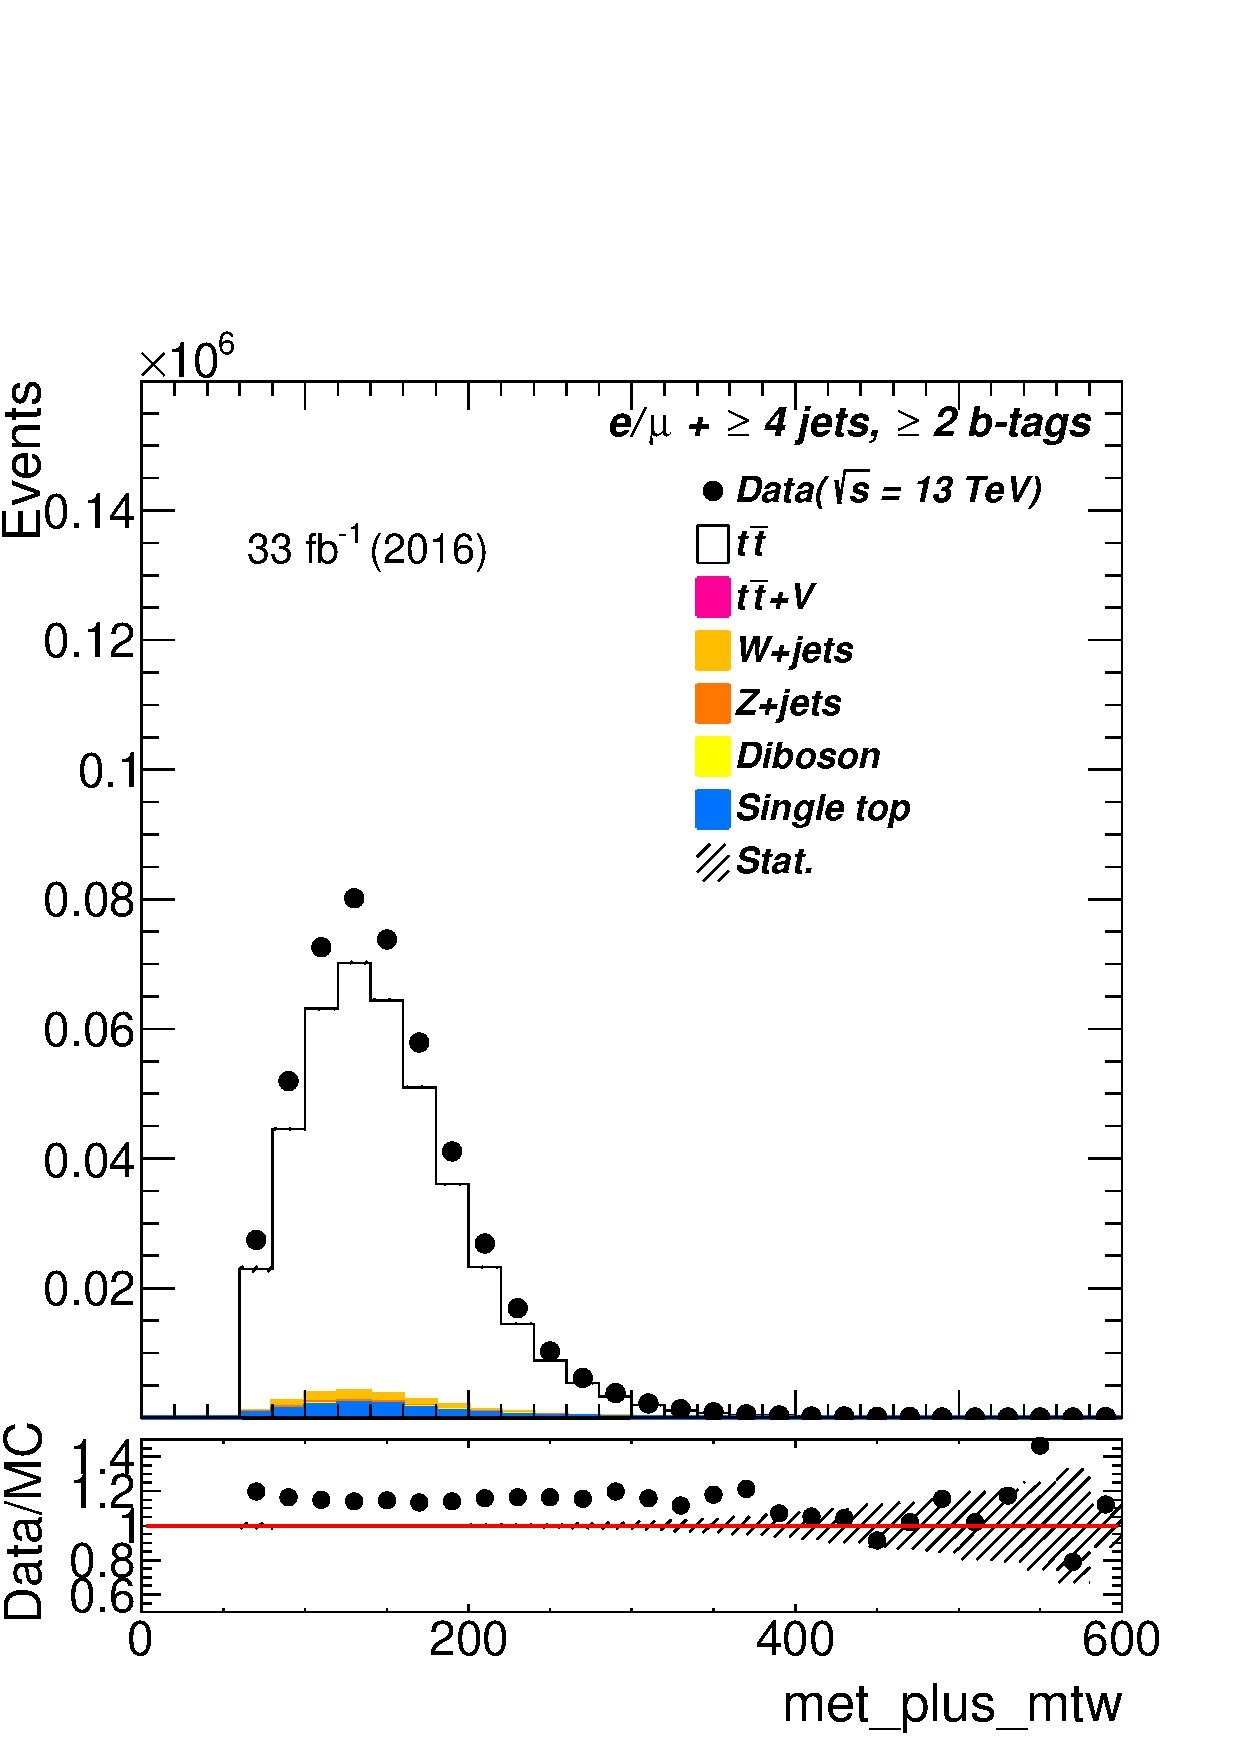
\includegraphics[width=\linewidth]{ControlPlots_emujets_2016_4incl_2incl/met_plus_mtw_emujets_2016.pdf}
\caption{$E_T^{\rm miss}$ + $W_T$-mass.} \label{fig:Sec3}
\end{subfigure}
	
	
\begin{subfigure}{0.25\textwidth}
	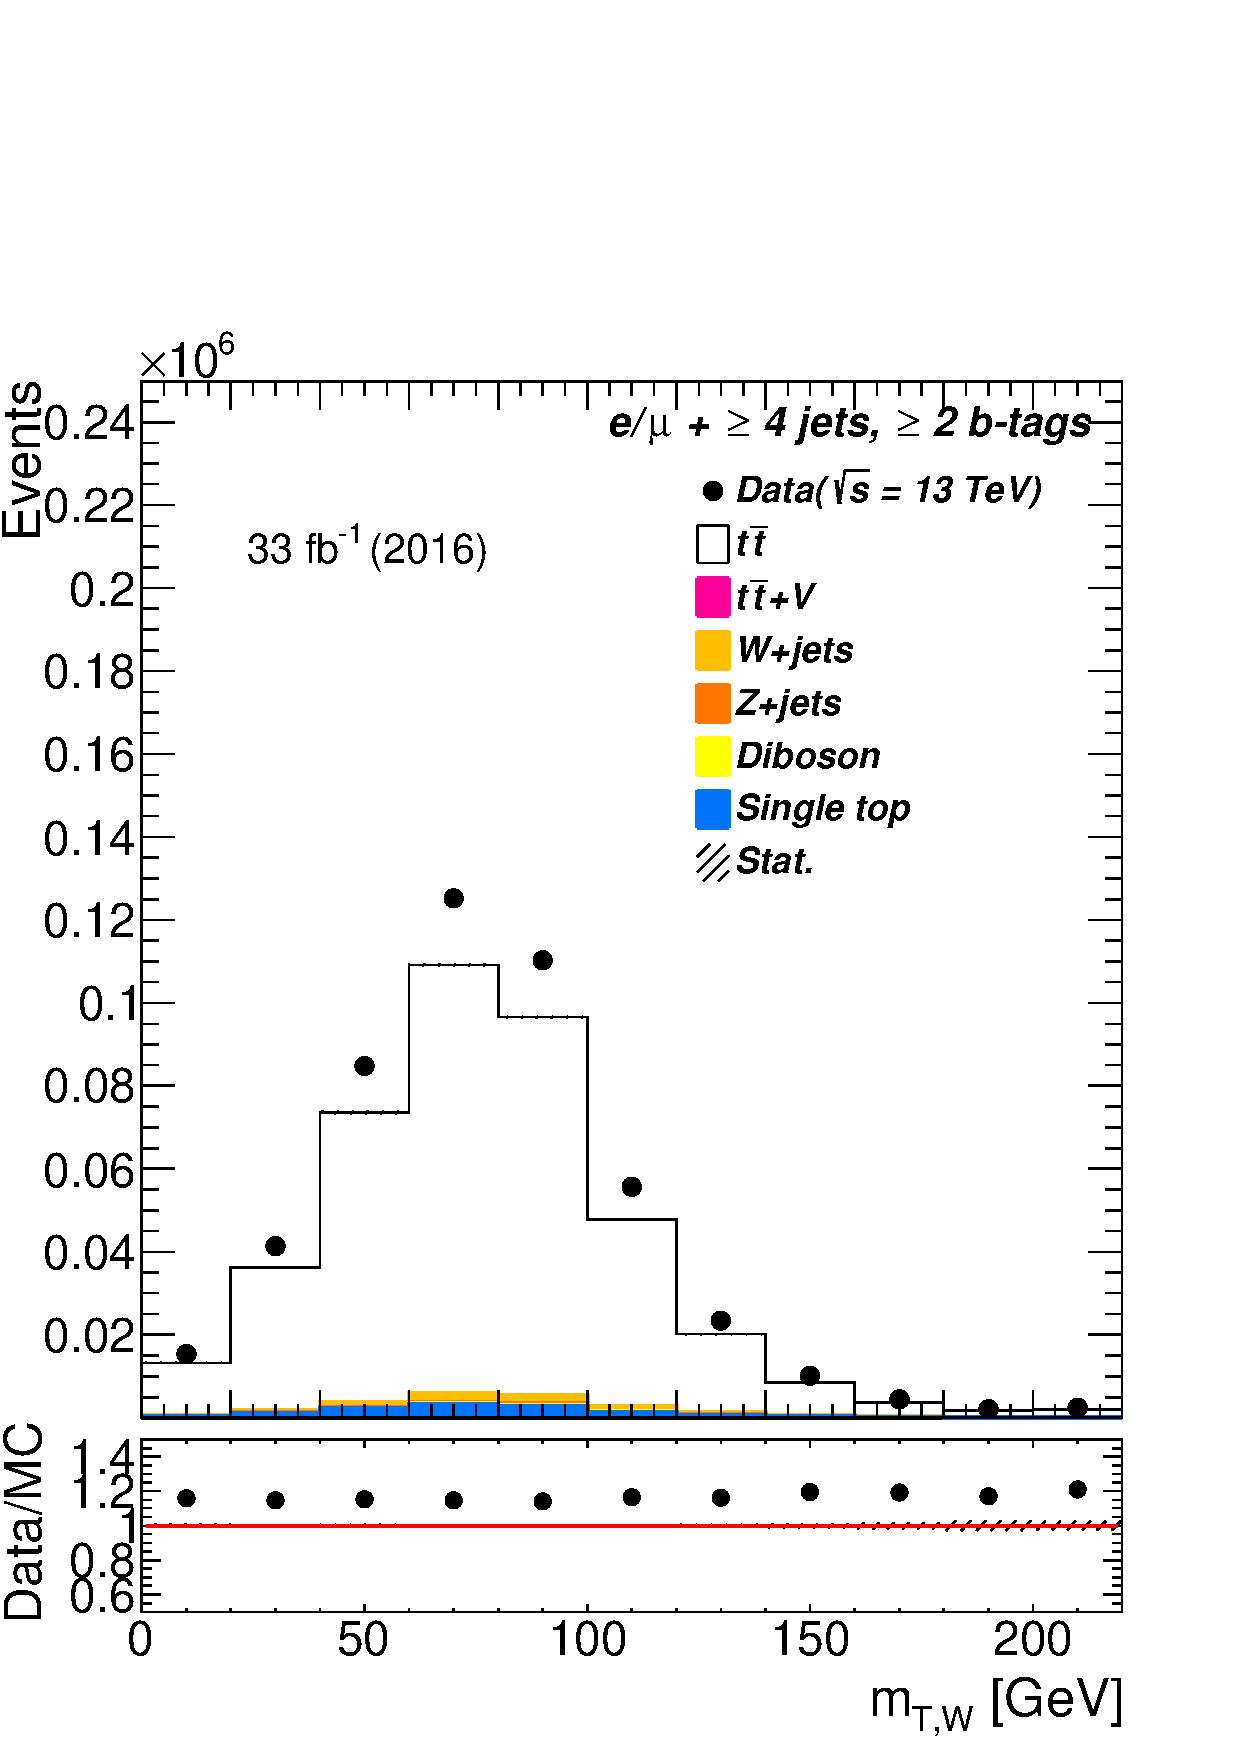
\includegraphics[width=\linewidth]{ControlPlots_emujets_2016_4incl_2incl/mtw_emujets_2016.png}
	\caption{Leptonic  $W_T$-mass.} \label{fig:Sec4}
\end{subfigure}
\hspace*{0.5cm}
\begin{subfigure}{0.25\textwidth}		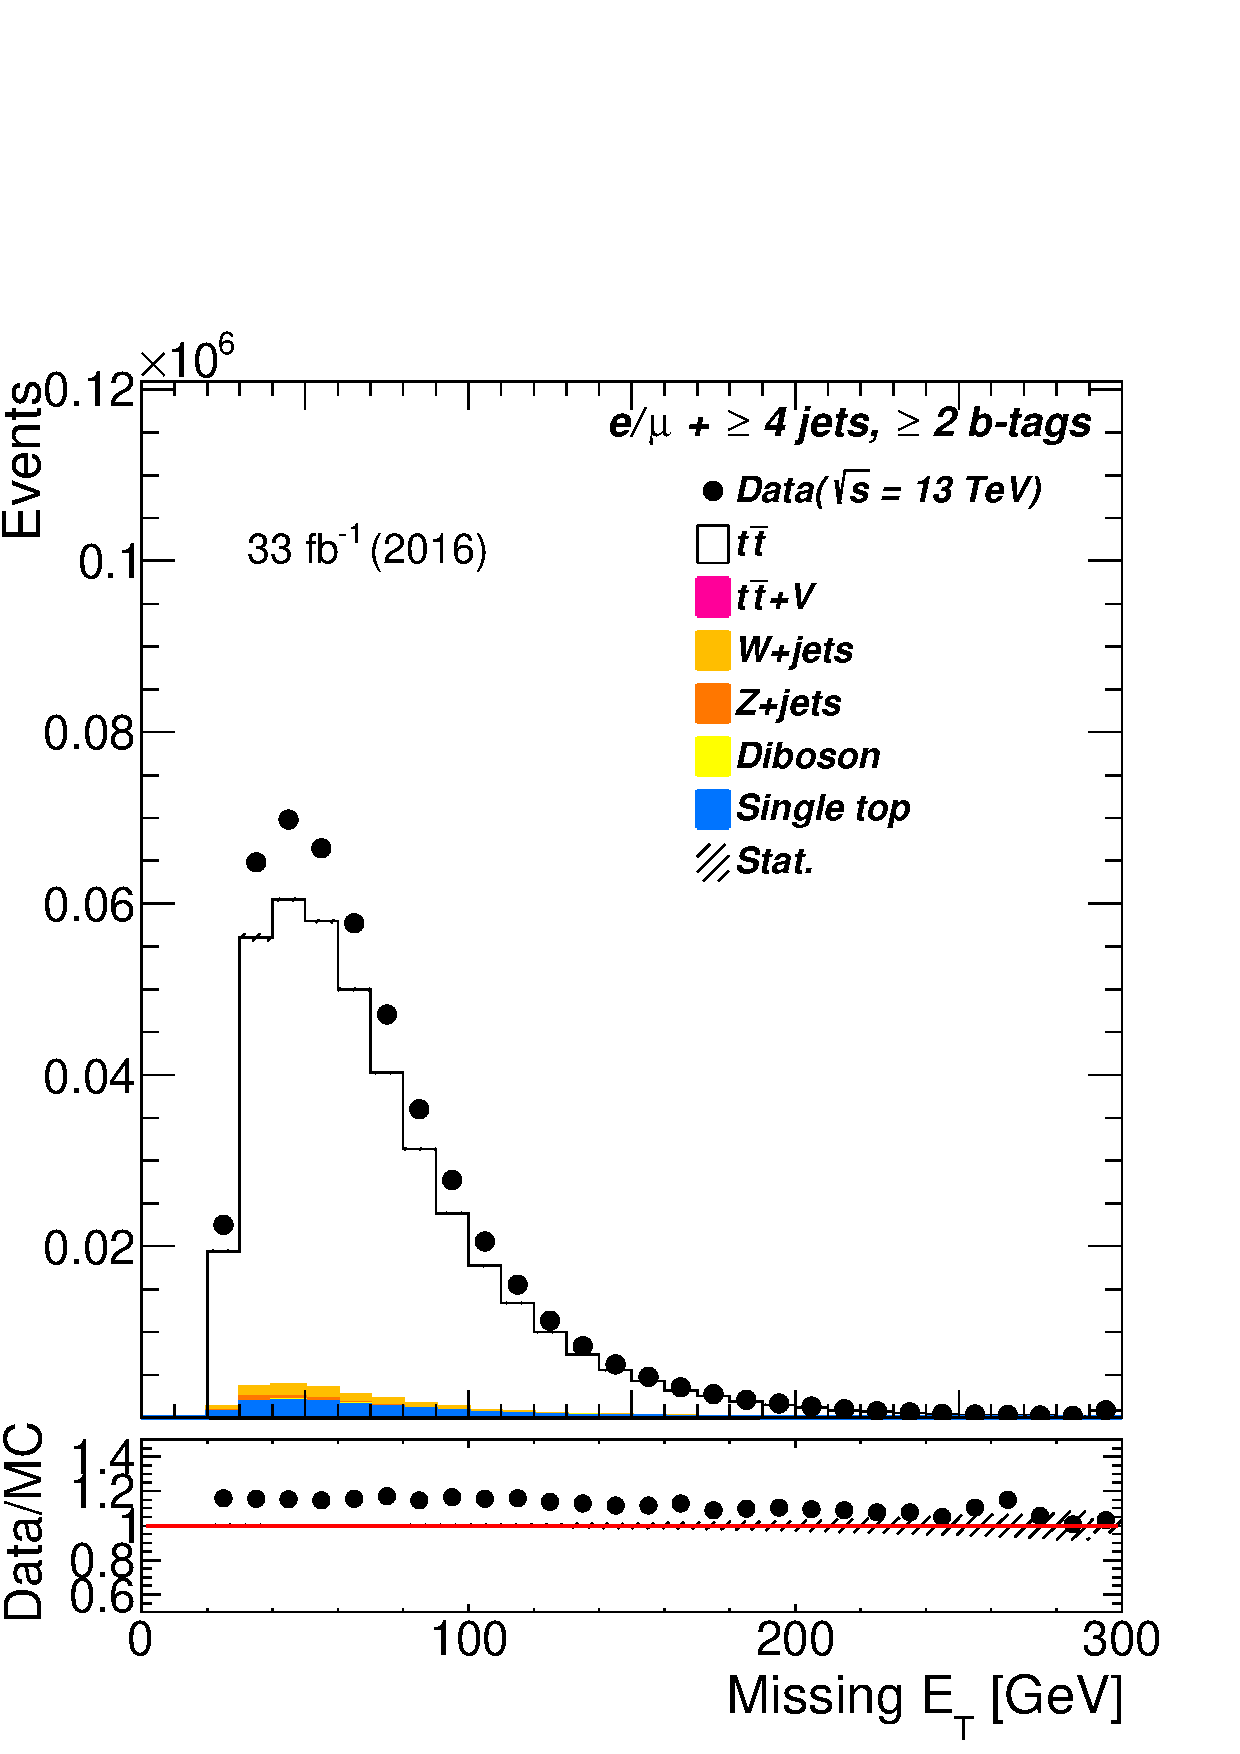
\includegraphics[width=\linewidth]{ControlPlots_emujets_2016_4incl_2incl/met_met_emujets_2016.png}
	 	\caption{$E_T^{\rm miss}$.} \label{fig:Sec5}
 \end{subfigure}
 \hspace*{0.5cm}
 	\begin{subfigure}{0.25\textwidth}
	 	\includegraphics[width=\linewidth]{ControlPlots_emujets_2016_4incl_2incl/met_phi_emujets_2016.png}
	 	\caption{$\phi$ of $E_T^{\rm miss}$.} \label{fig:Sec6}
	 \end{subfigure}

 
 

 \begin{subfigure}{0.25\textwidth}
 	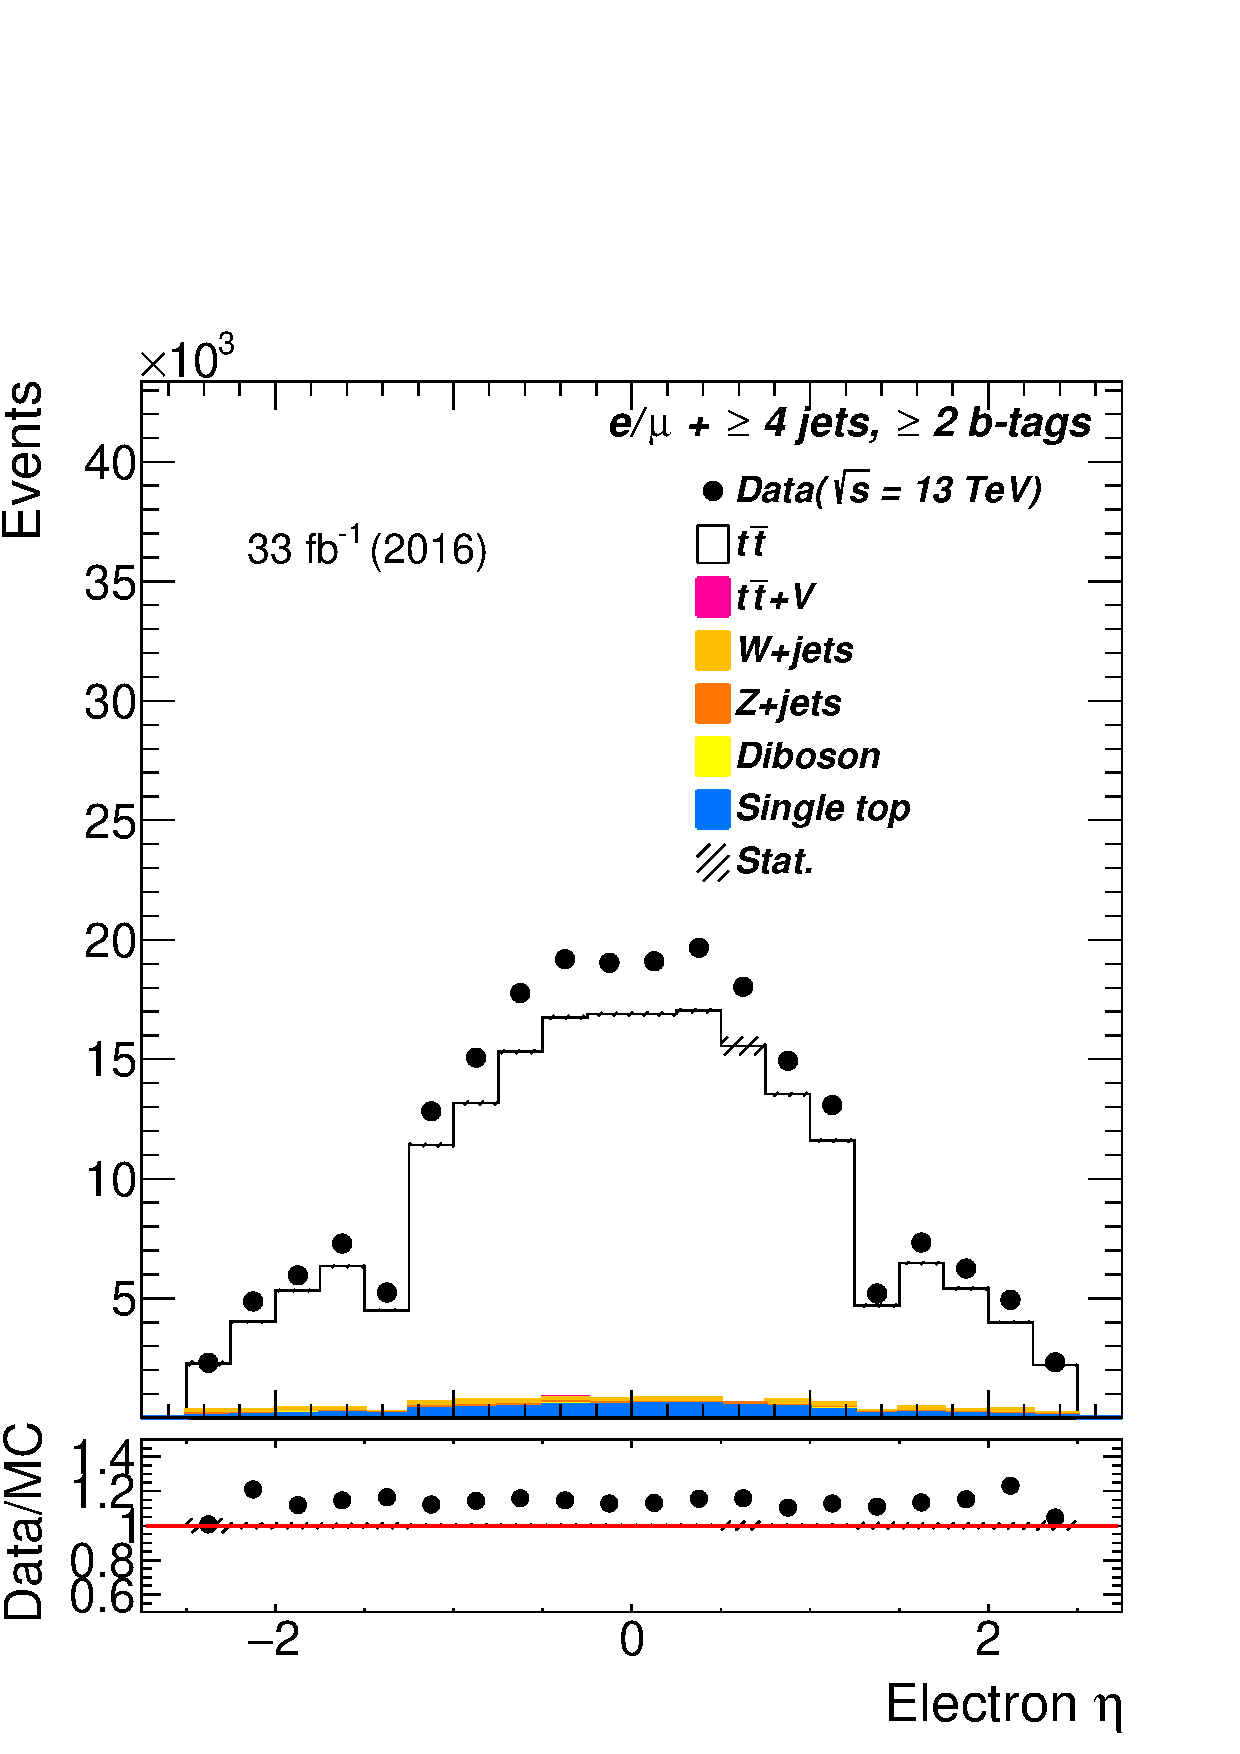
\includegraphics[width=\linewidth]{ControlPlots_emujets_2016_4incl_2incl/el_eta_emujets_2016.png}
 	\caption{$\eta$ of the electrons.} \label{fig:Sec9}
 \end{subfigure}\hspace*{0.5cm}
 \begin{subfigure}{0.25\textwidth}
 	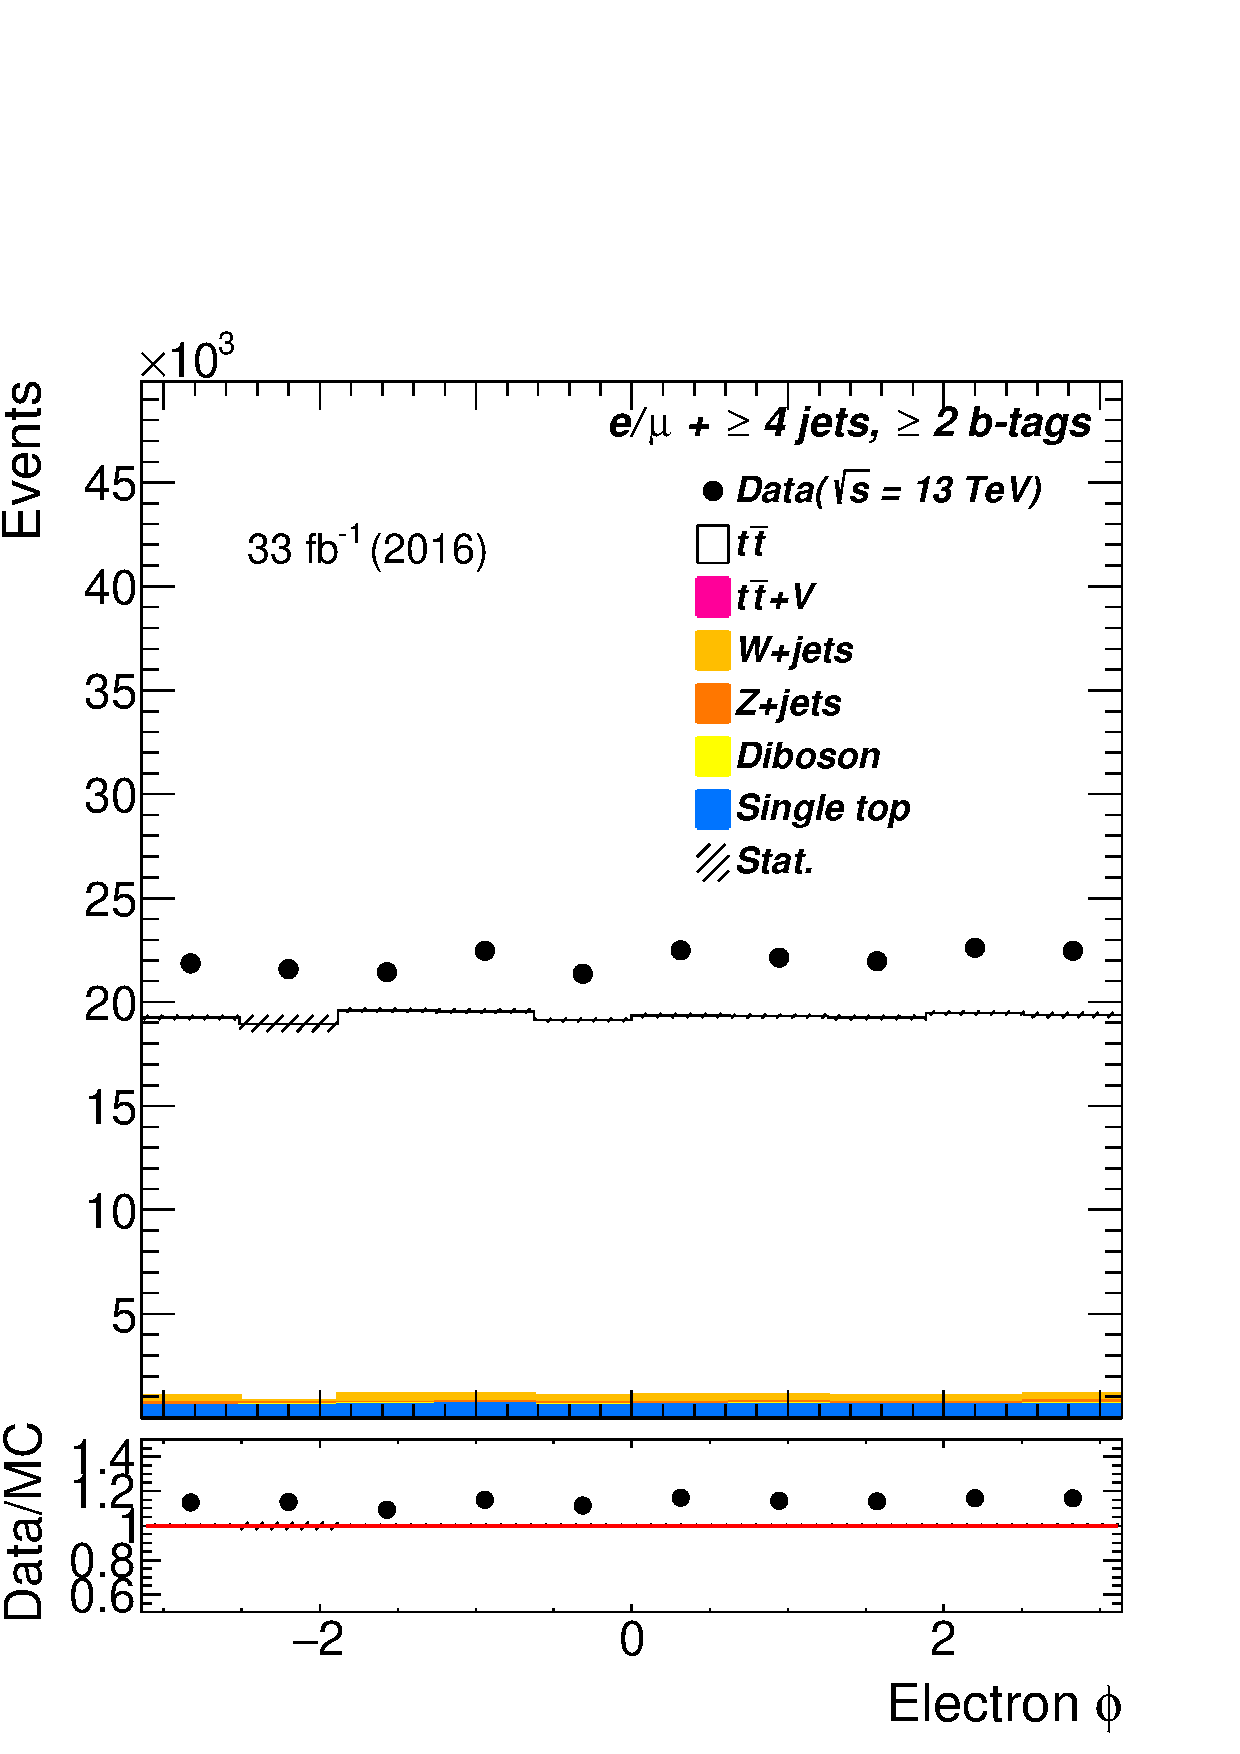
\includegraphics[width=\linewidth]{ControlPlots_emujets_2016_4incl_2incl/el_phi_emujets_2016.png}
 	\caption{$\phi$ of the electrons.} \label{fig:Sec10}
 \end{subfigure}\hspace*{0.5cm}
 \begin{subfigure}{0.25\textwidth}
 	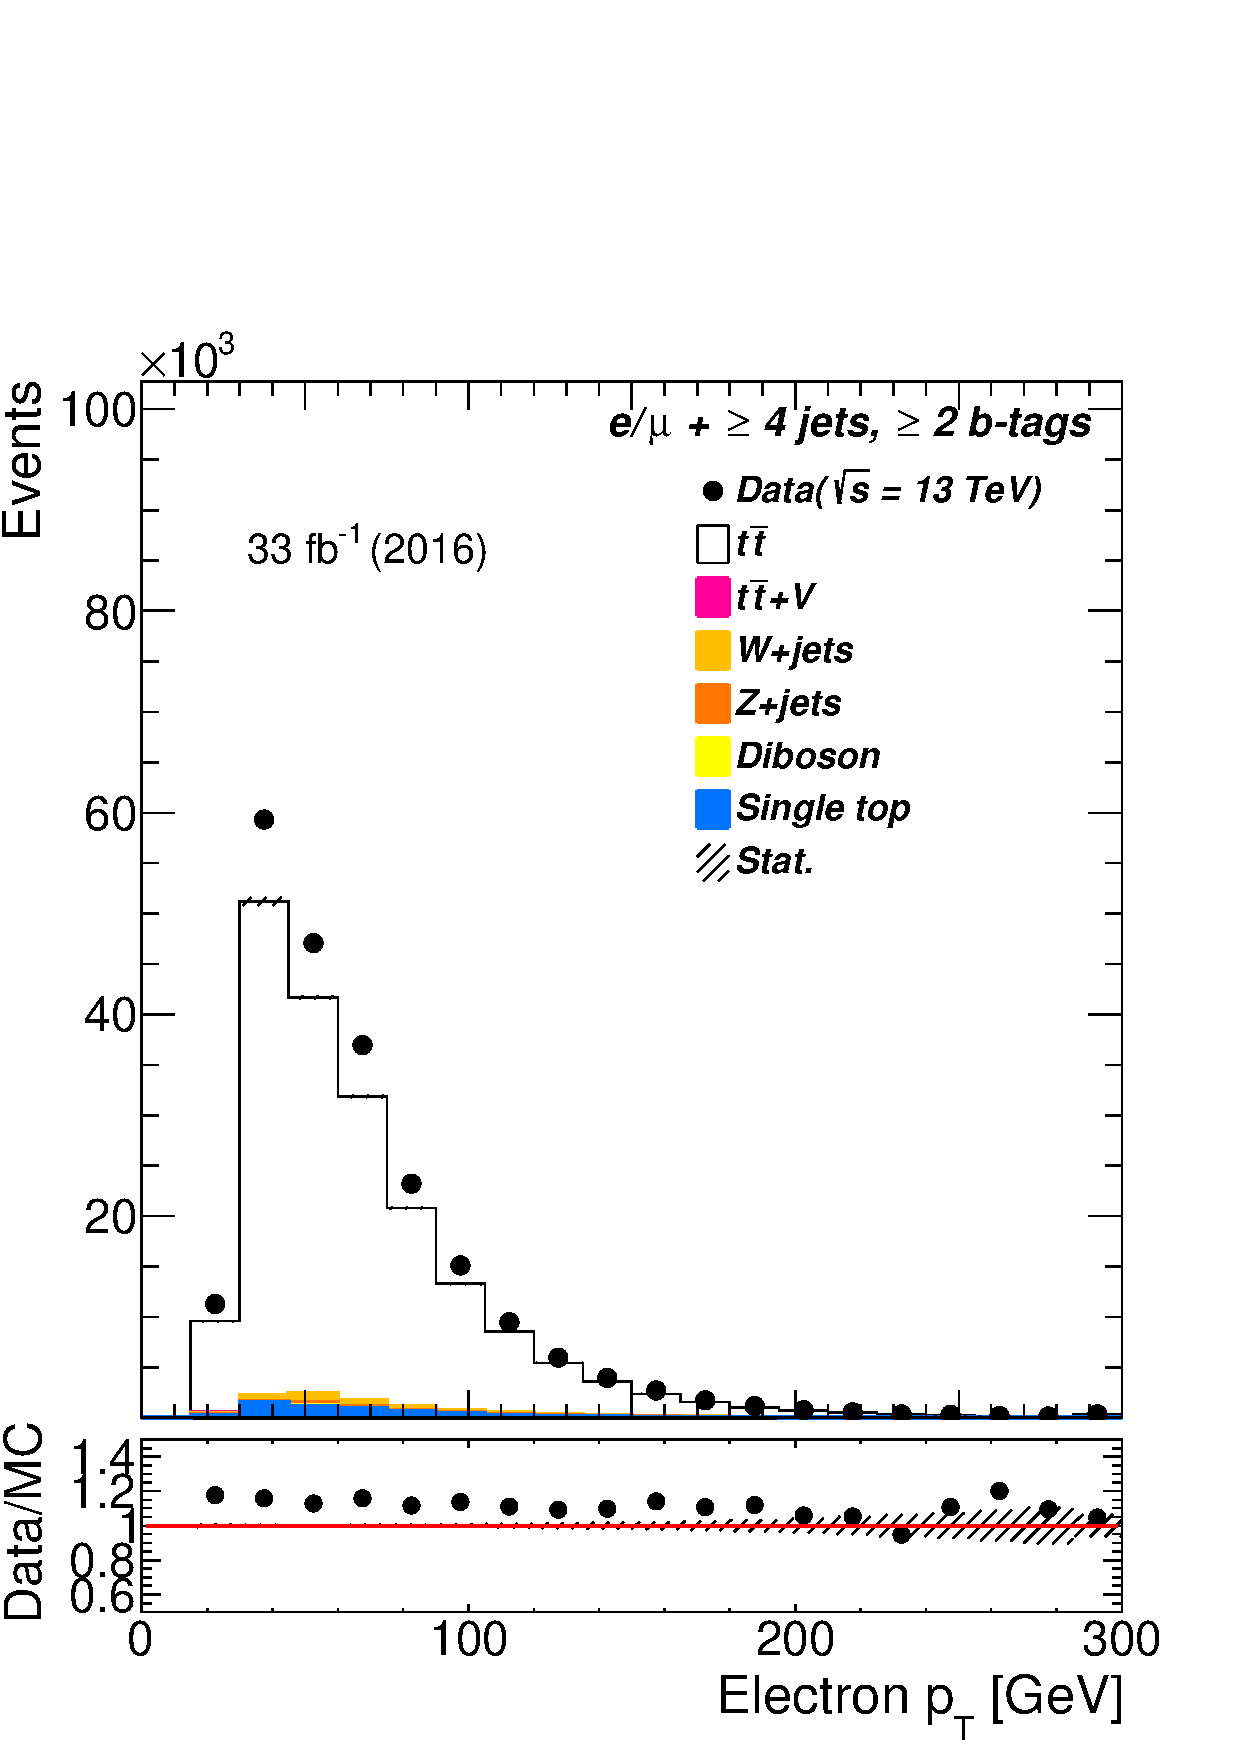
\includegraphics[width=\linewidth]{ControlPlots_emujets_2016_4incl_2incl/el_pt_emujets_2016.png}
 	\caption{Electron $p_T$.} \label{fig:Sec13}
 \end{subfigure}
 
 
 	
	\caption{Observed distributions after the event preselection. All events are observed in the lepton + jets decay channel and contain at least 4 jets and at least two $b$-tagged jets. The data is displayed by the black points. The solid histogram shows the signal-plus background predicted events, which are normalized to the number of events observed in data. The lower part shows the data-simulation agreement.}
	\label{fig:Sel1}
\end{figure}	


\begin{figure} % "[t!]" placement specifier just for this example
	\centering	


	\begin{subfigure}{0.25\textwidth}
	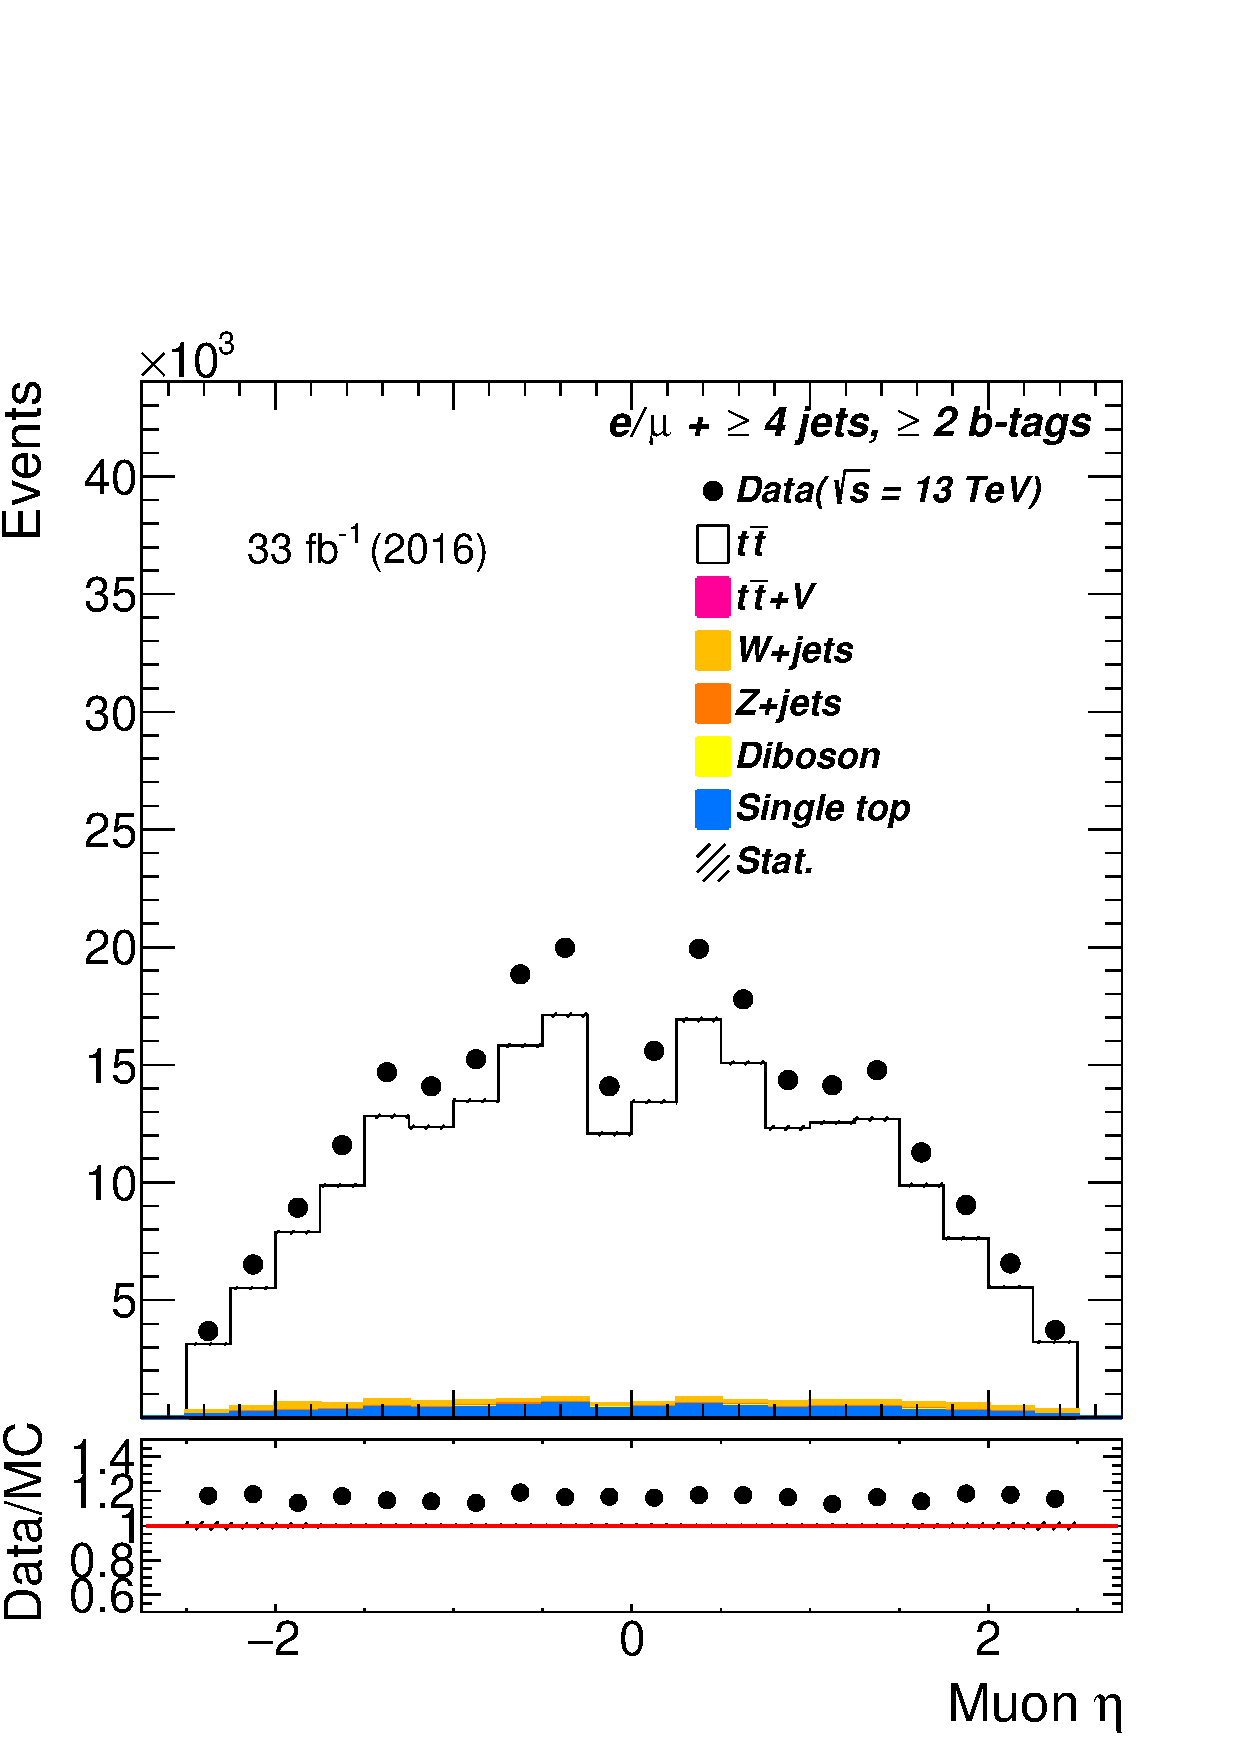
\includegraphics[width=\linewidth]{ControlPlots_emujets_2016_4incl_2incl/mu_eta_emujets_2016.png}
	\caption{$\eta$ the muons} \label{fig:Sec17}
\end{subfigure}\hspace*{0.5cm}
		\begin{subfigure}{0.25\textwidth}
	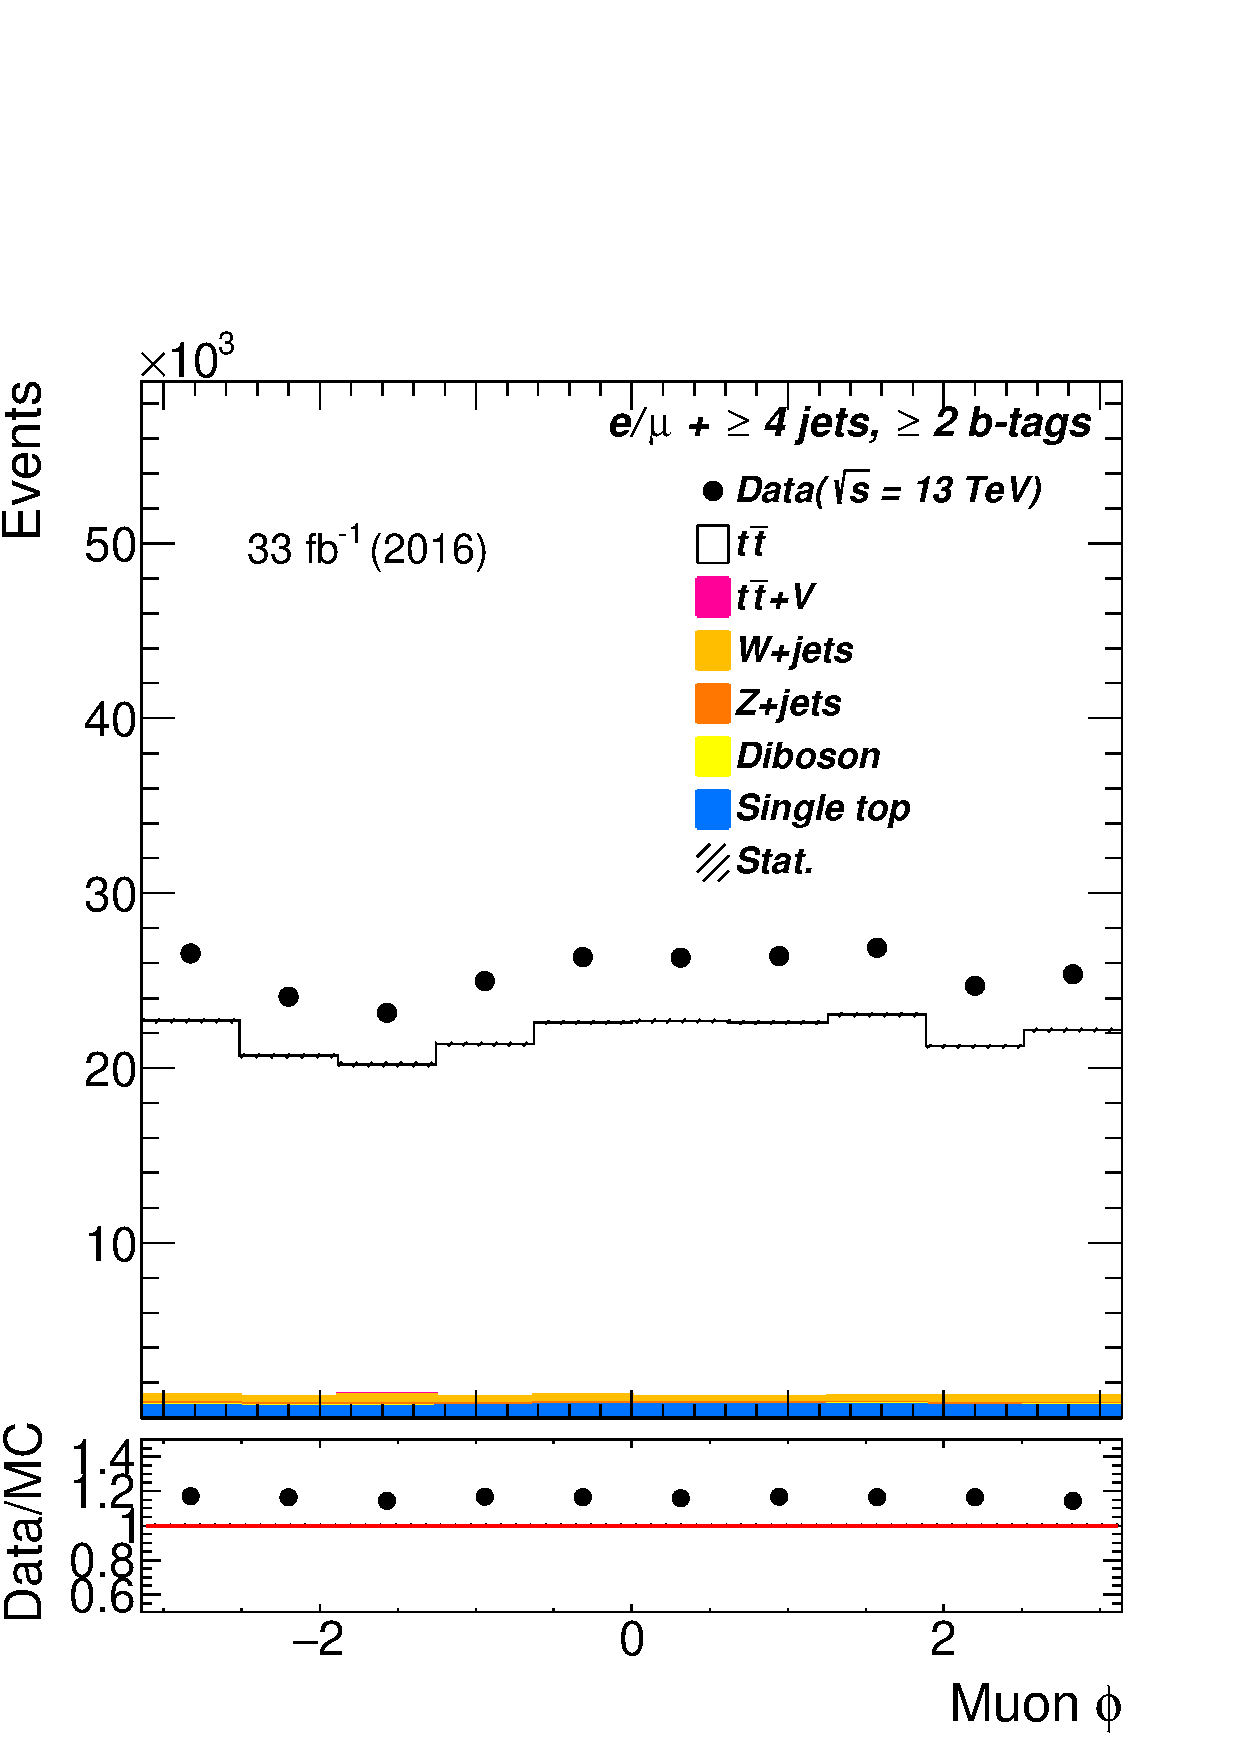
\includegraphics[width=\linewidth]{ControlPlots_emujets_2016_4incl_2incl/mu_phi_emujets_2016.png}
	\caption{$\phi$ of the muons.} \label{fig:Sec18}
\end{subfigure}\hspace*{0.5cm}
	\begin{subfigure}{0.25\textwidth}
		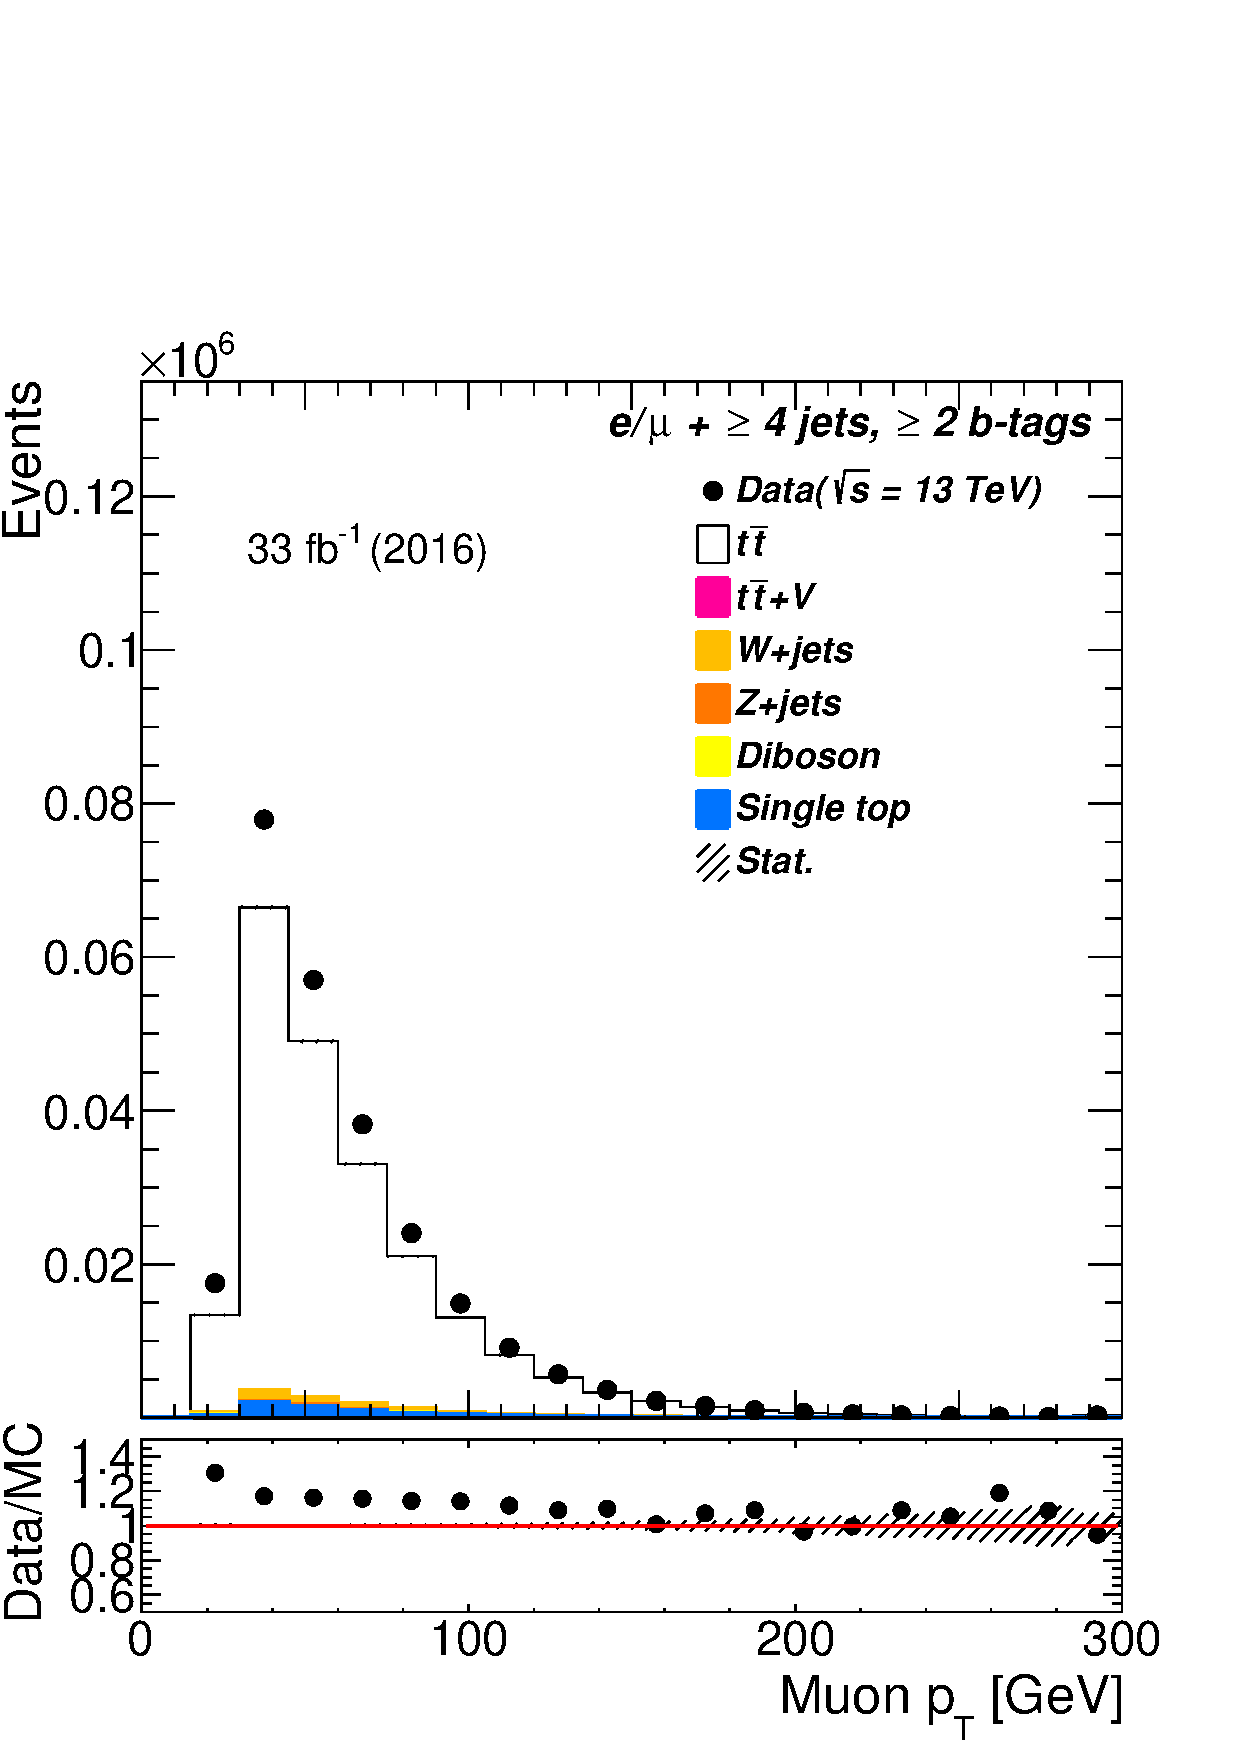
\includegraphics[width=\linewidth]{ControlPlots_emujets_2016_4incl_2incl/mu_pt_emujets_2016.png}
		\caption{Muon $p_T$.} \label{fig:Sec12}
	\end{subfigure}


	\begin{subfigure}{0.25\textwidth}
		\includegraphics[width=\linewidth]{ControlPlots_emujets_2016_4incl_2incl/jet0_eta_emujets_2016.png}
		\caption{$\eta$ the first jet.} \label{fig:Sec19}
	\end{subfigure}\hspace*{0.5cm}
\begin{subfigure}{0.25\textwidth}
	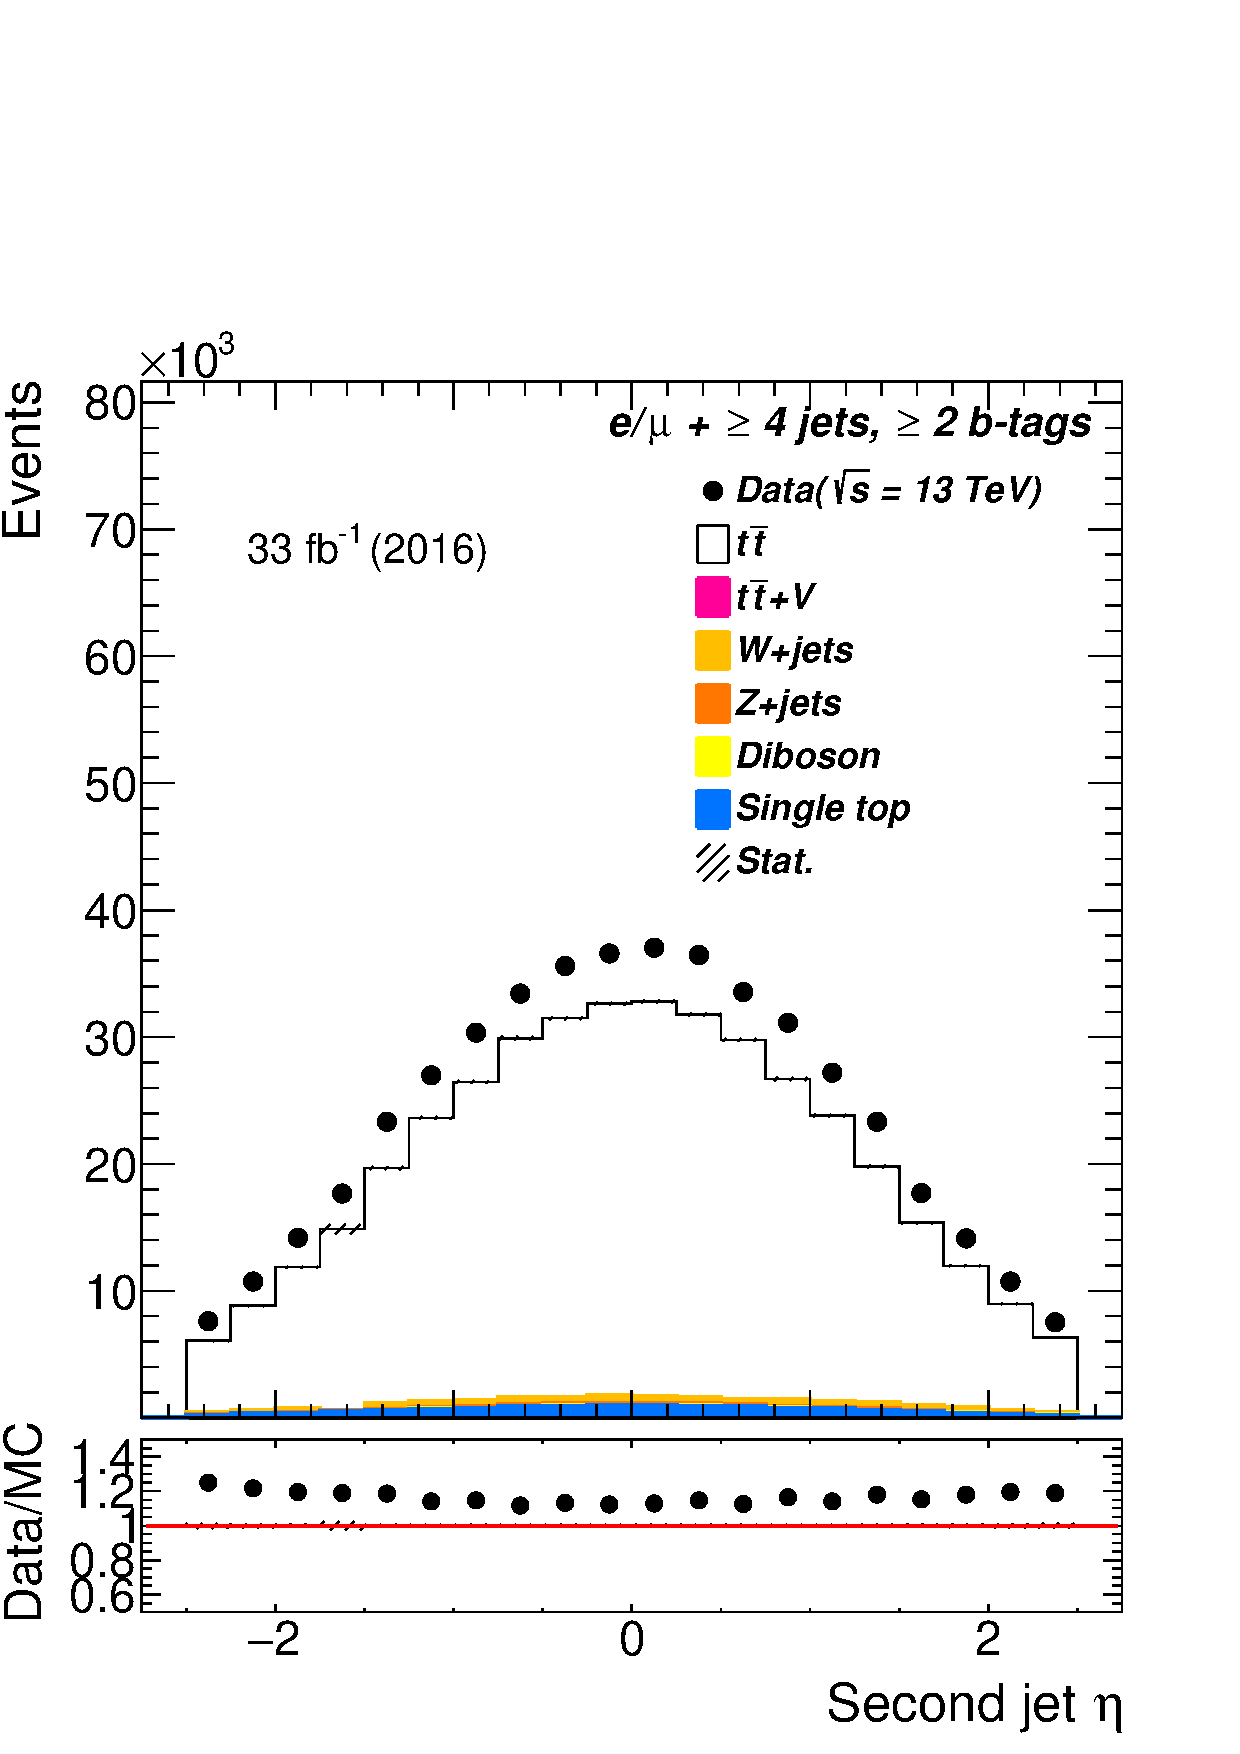
\includegraphics[width=\linewidth]{ControlPlots_emujets_2016_4incl_2incl/jet1_eta_emujets_2016.png}
	\caption{$\eta$ of the sec. jet.} \label{figSec23}
\end{subfigure}
\begin{subfigure}{0.25\textwidth}
	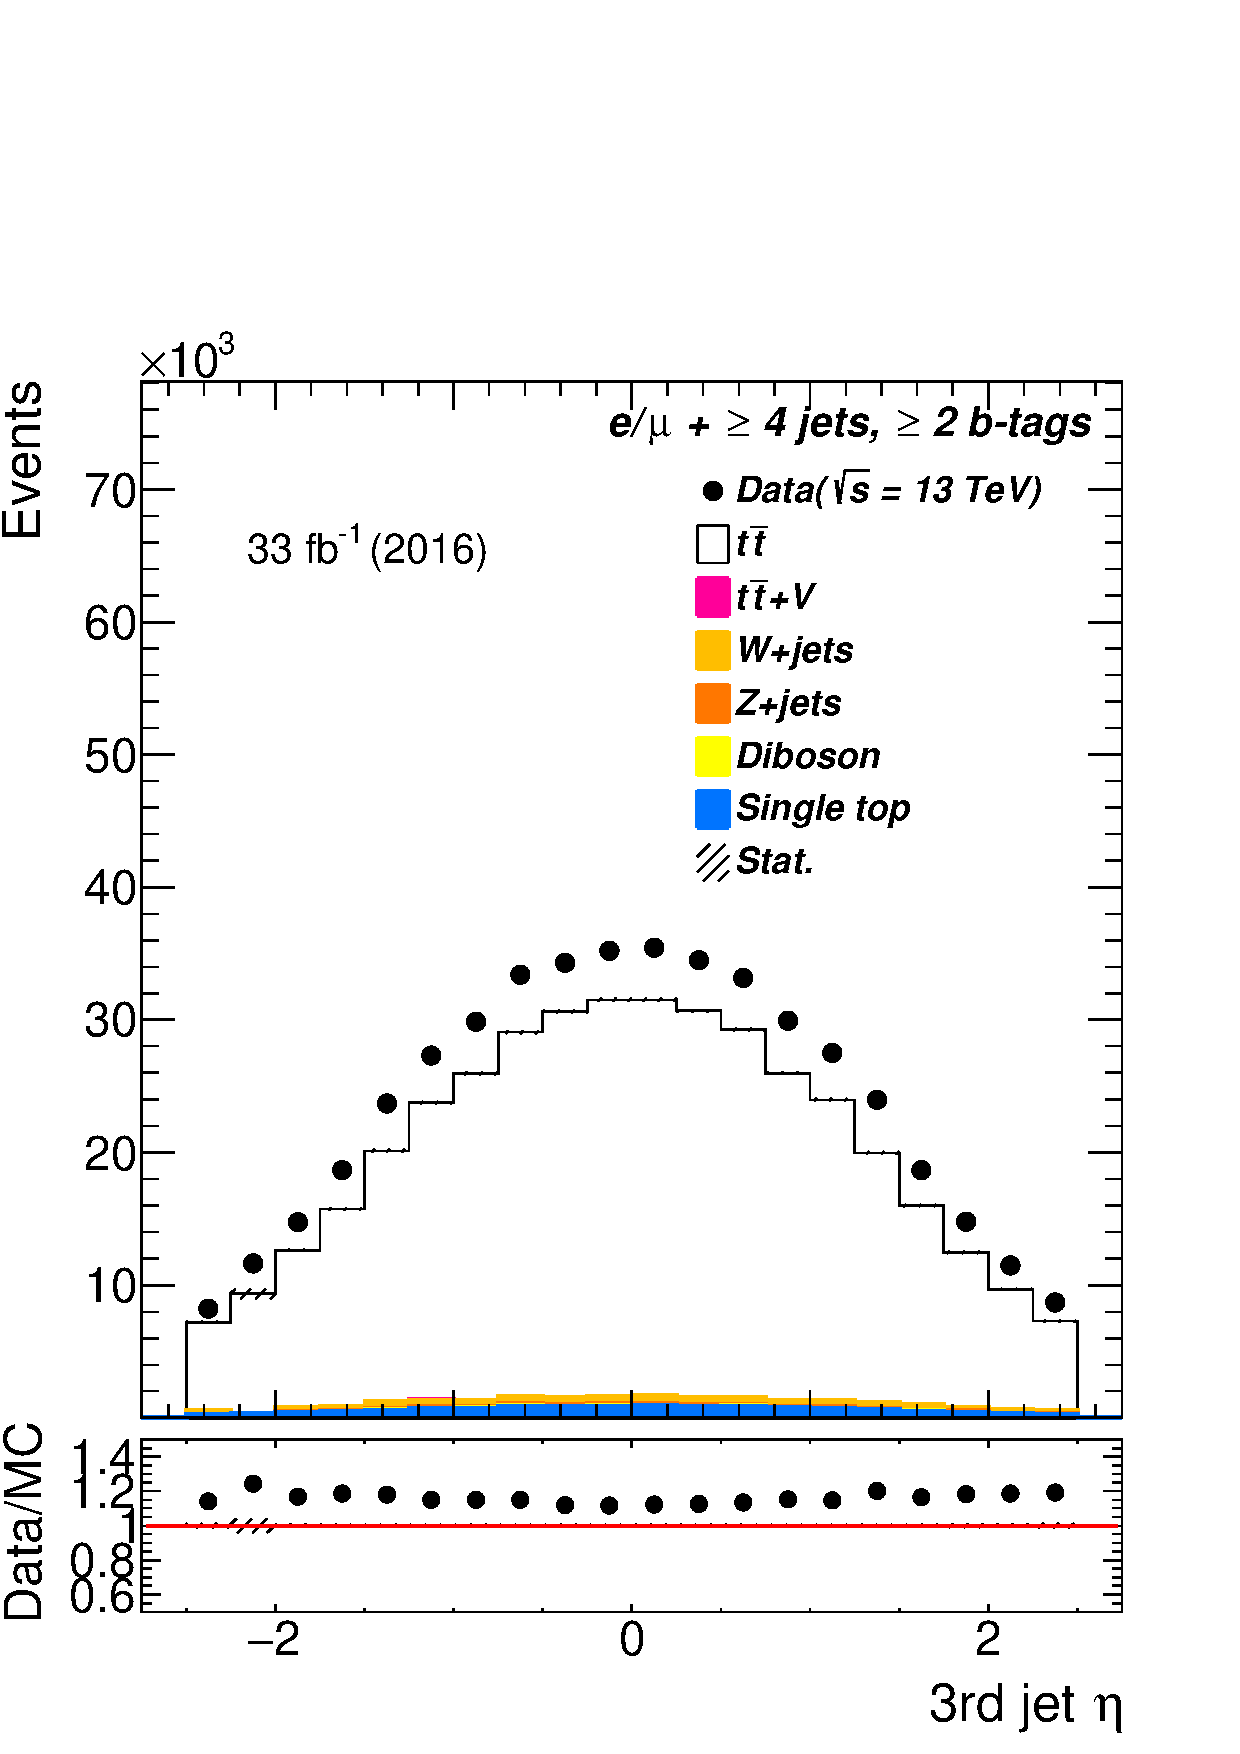
\includegraphics[width=\linewidth]{ControlPlots_emujets_2016_4incl_2incl/jet2_eta_emujets_2016.png}
	\caption{$\eta$ of the third jet.} \label{fig:Sec25}
\end{subfigure}

\begin{subfigure}{0.25\textwidth}
	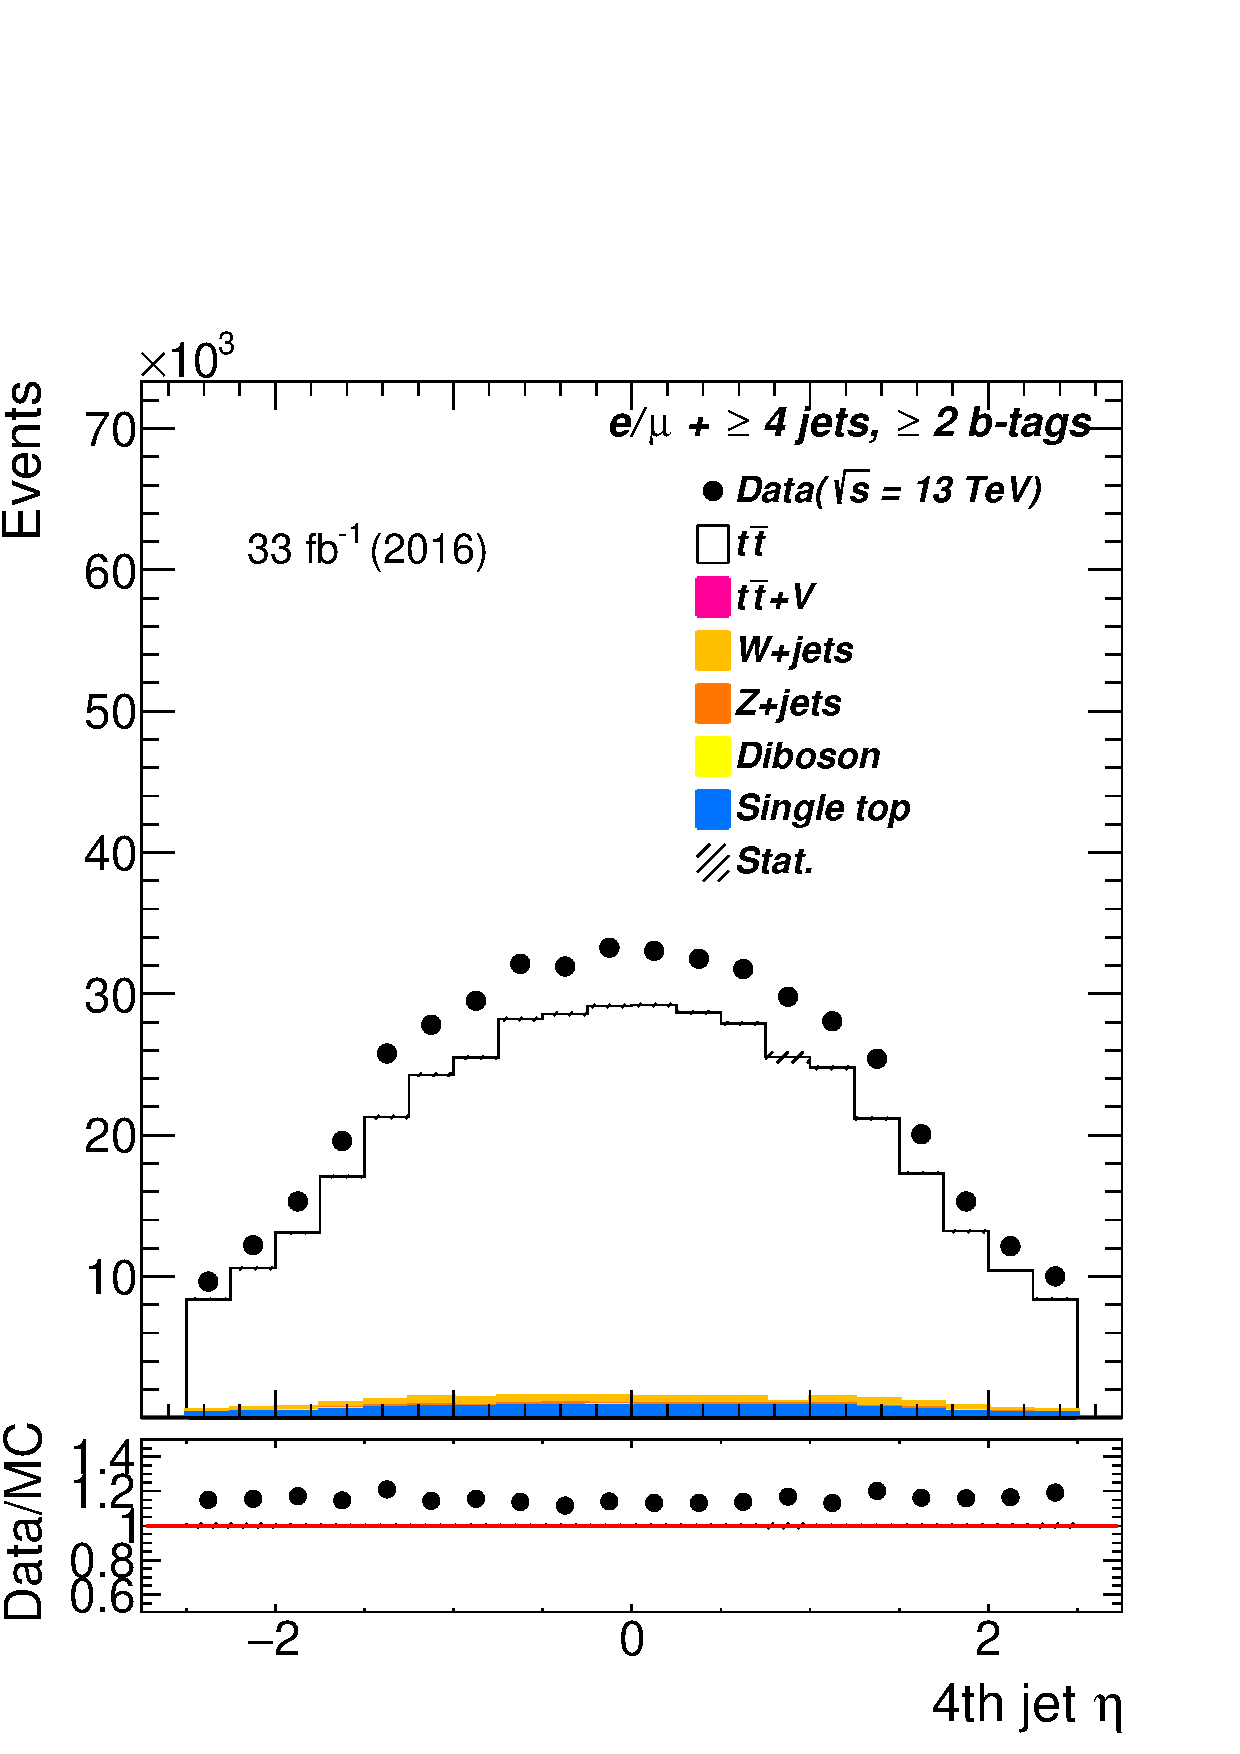
\includegraphics[width=\linewidth]{ControlPlots_emujets_2016_4incl_2incl/jet3_eta_emujets_2016.png}
	\caption{$\eta$ of the fourth jet.} \label{fig:Sec29}
\end{subfigure}



	
	\caption{As in~\cref{fig:Sel1}, global distributions are displayed for the muon, as well as for the four jets, obtained for the sample with at least 4 jets and at last two $b$-tagged jets.}	\label{fig:Sel2}
\end{figure}















\clearpage

\begin{figure} [t]% "[t!]" placement specifier just for this example
	\centering
	
	
	
	
	\begin{subfigure}{0.25\textwidth}
		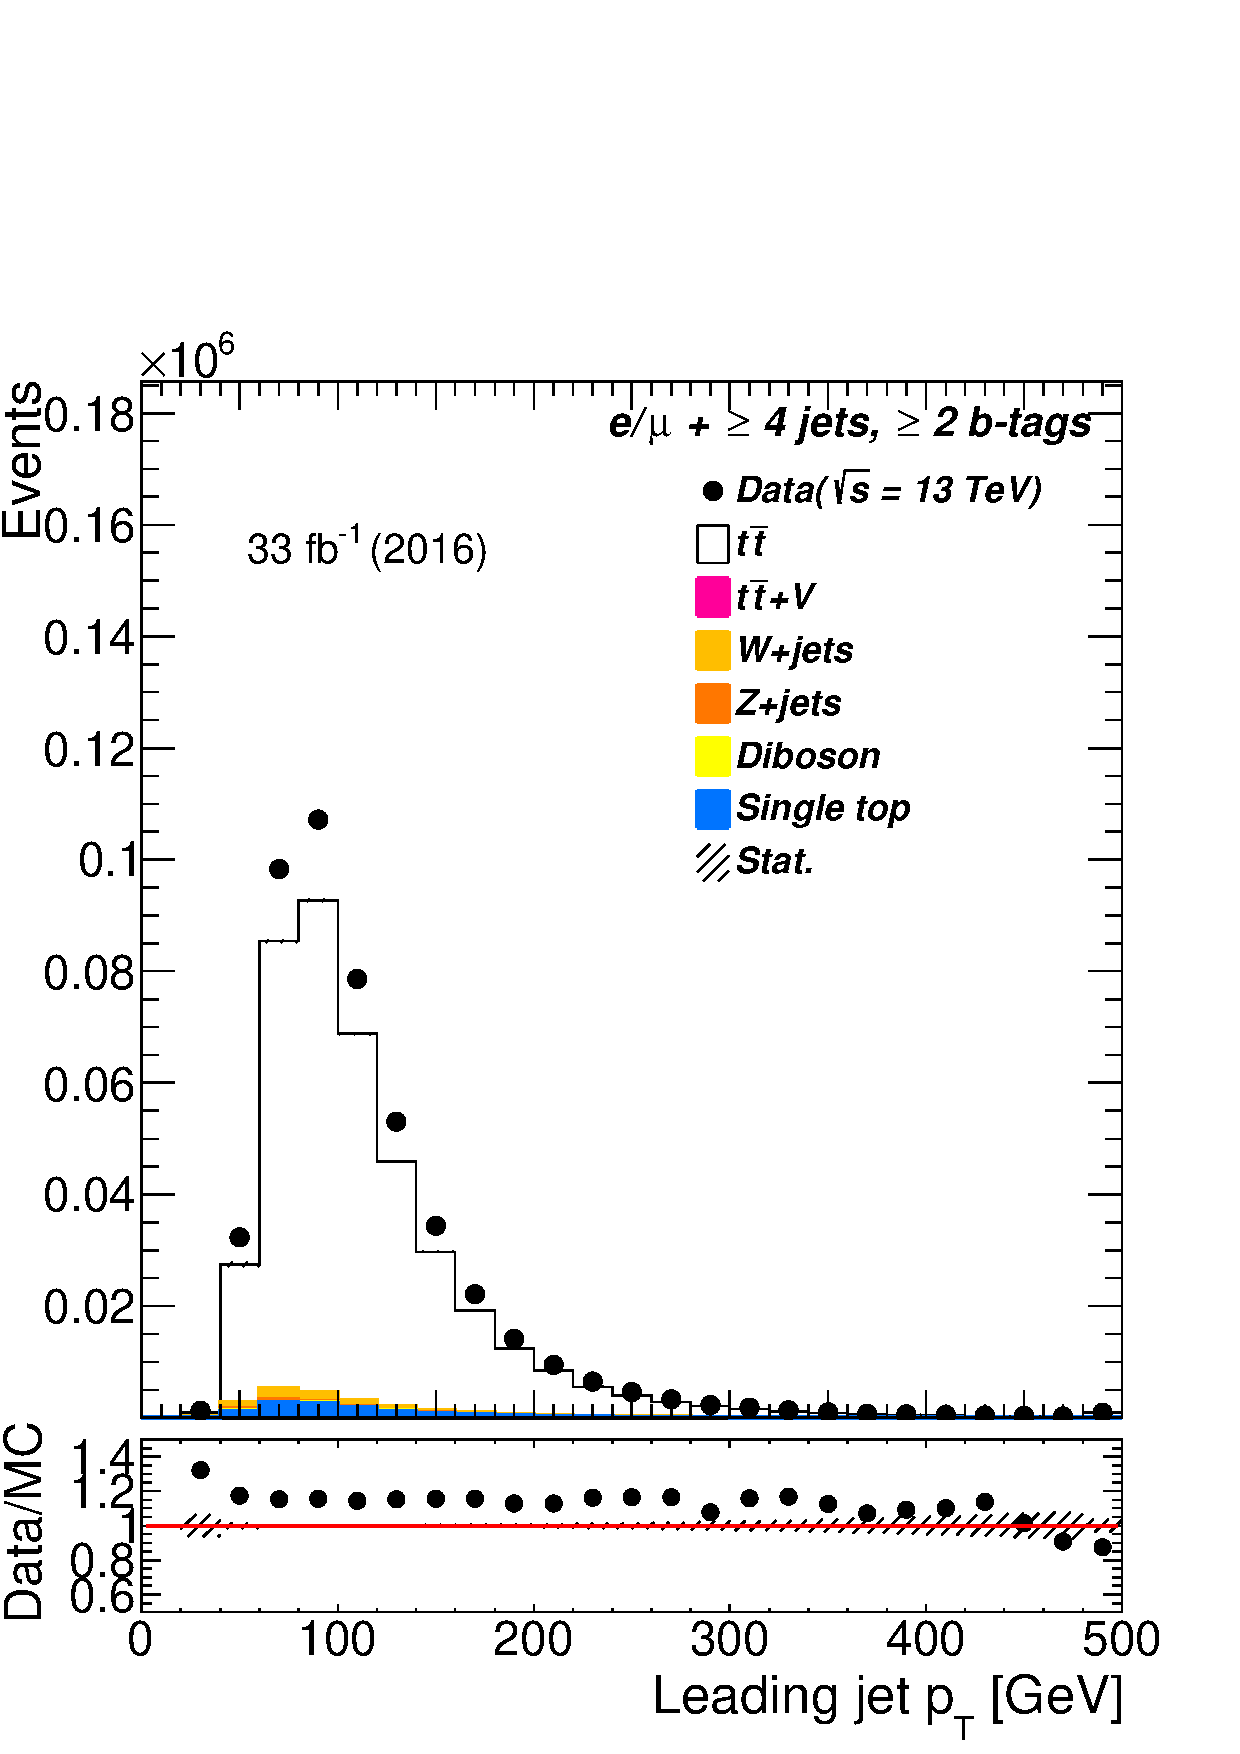
\includegraphics[width=\linewidth]{ControlPlots_emujets_2016_4incl_2incl/jet0_pt_emujets_2016.png}
		\caption{$p_T$ of the first jet.} \label{fig:Sec21}
	\end{subfigure}\hspace*{0.5cm}
	\begin{subfigure}{0.25\textwidth}
		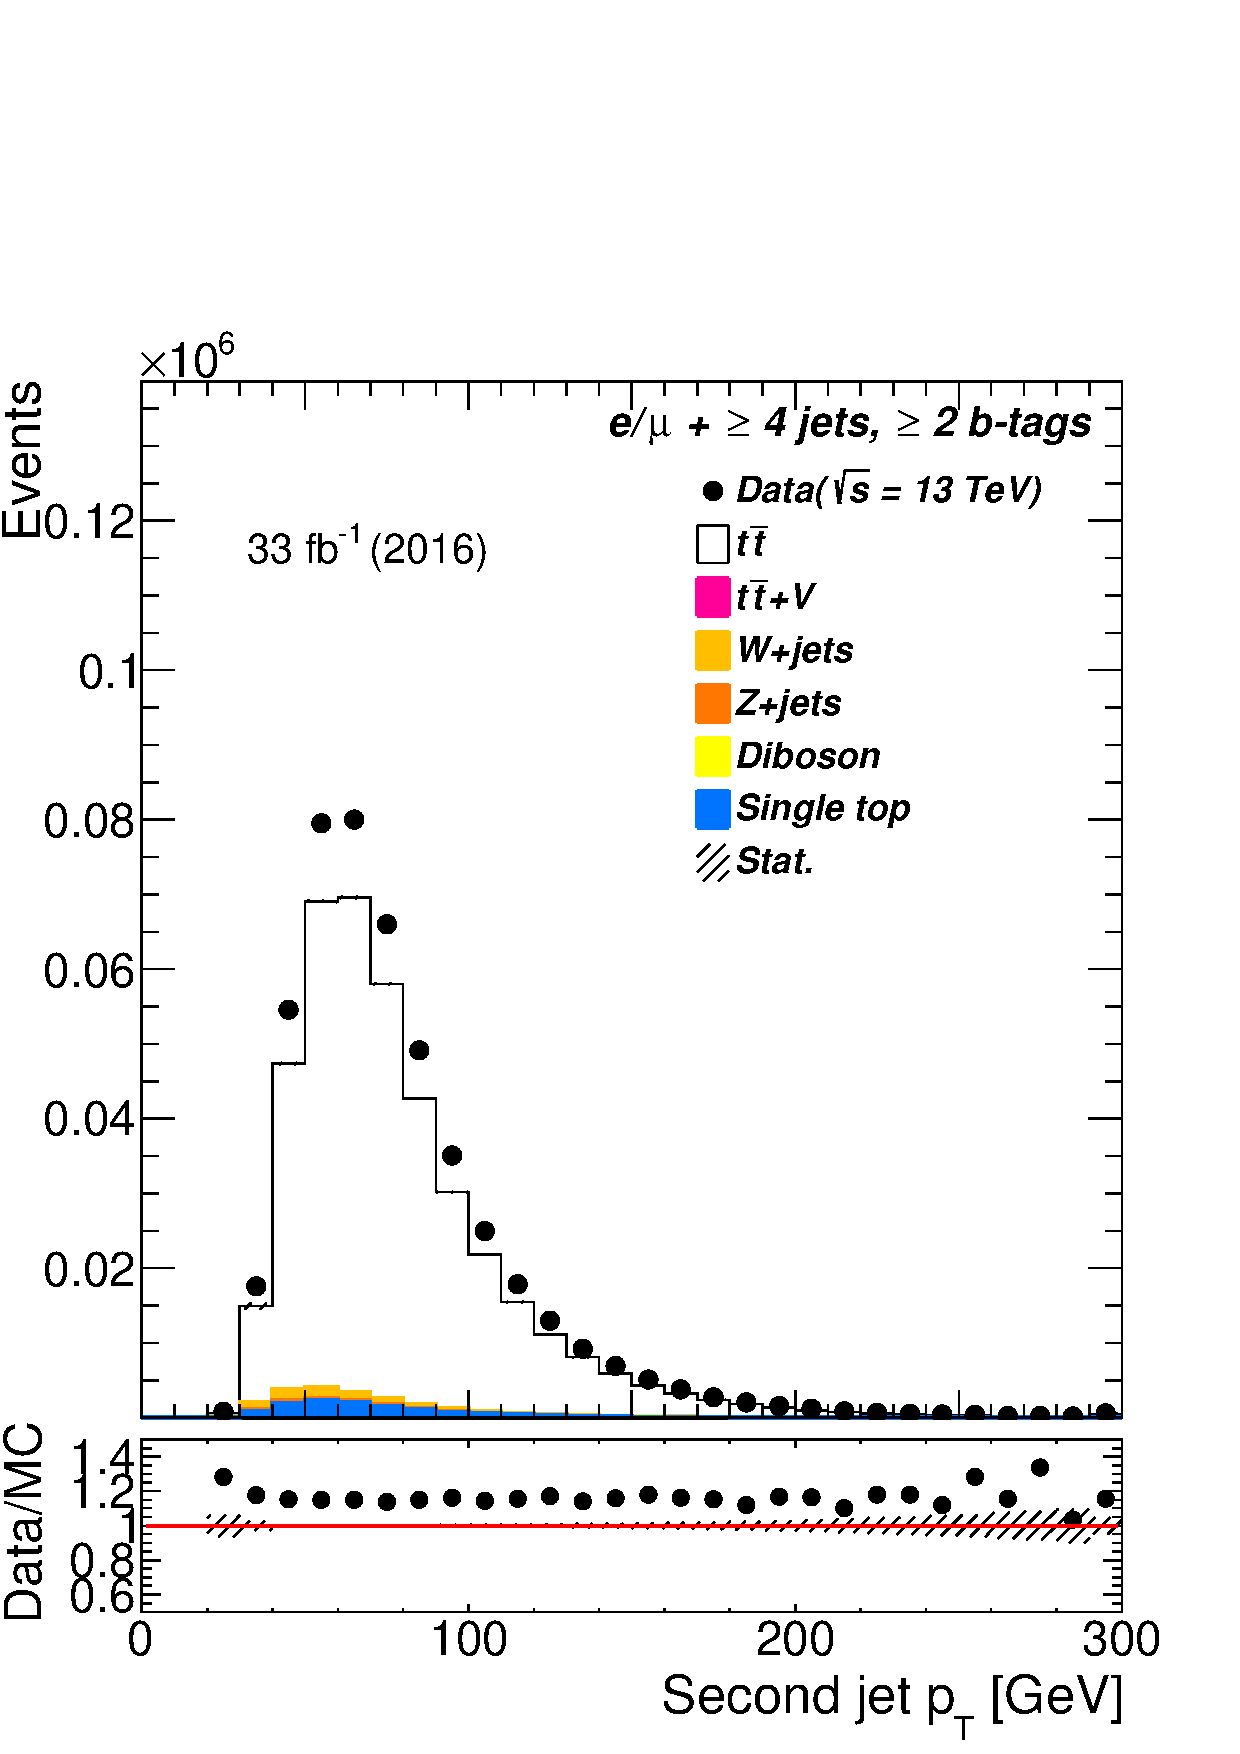
\includegraphics[width=\linewidth]{ControlPlots_emujets_2016_4incl_2incl/jet1_pt_emujets_2016.png}
		\caption{$p_T$ of the second jet.} \label{fig:Sec22}	
	\end{subfigure}
	
	
	
	\begin{subfigure}{0.25\textwidth}
		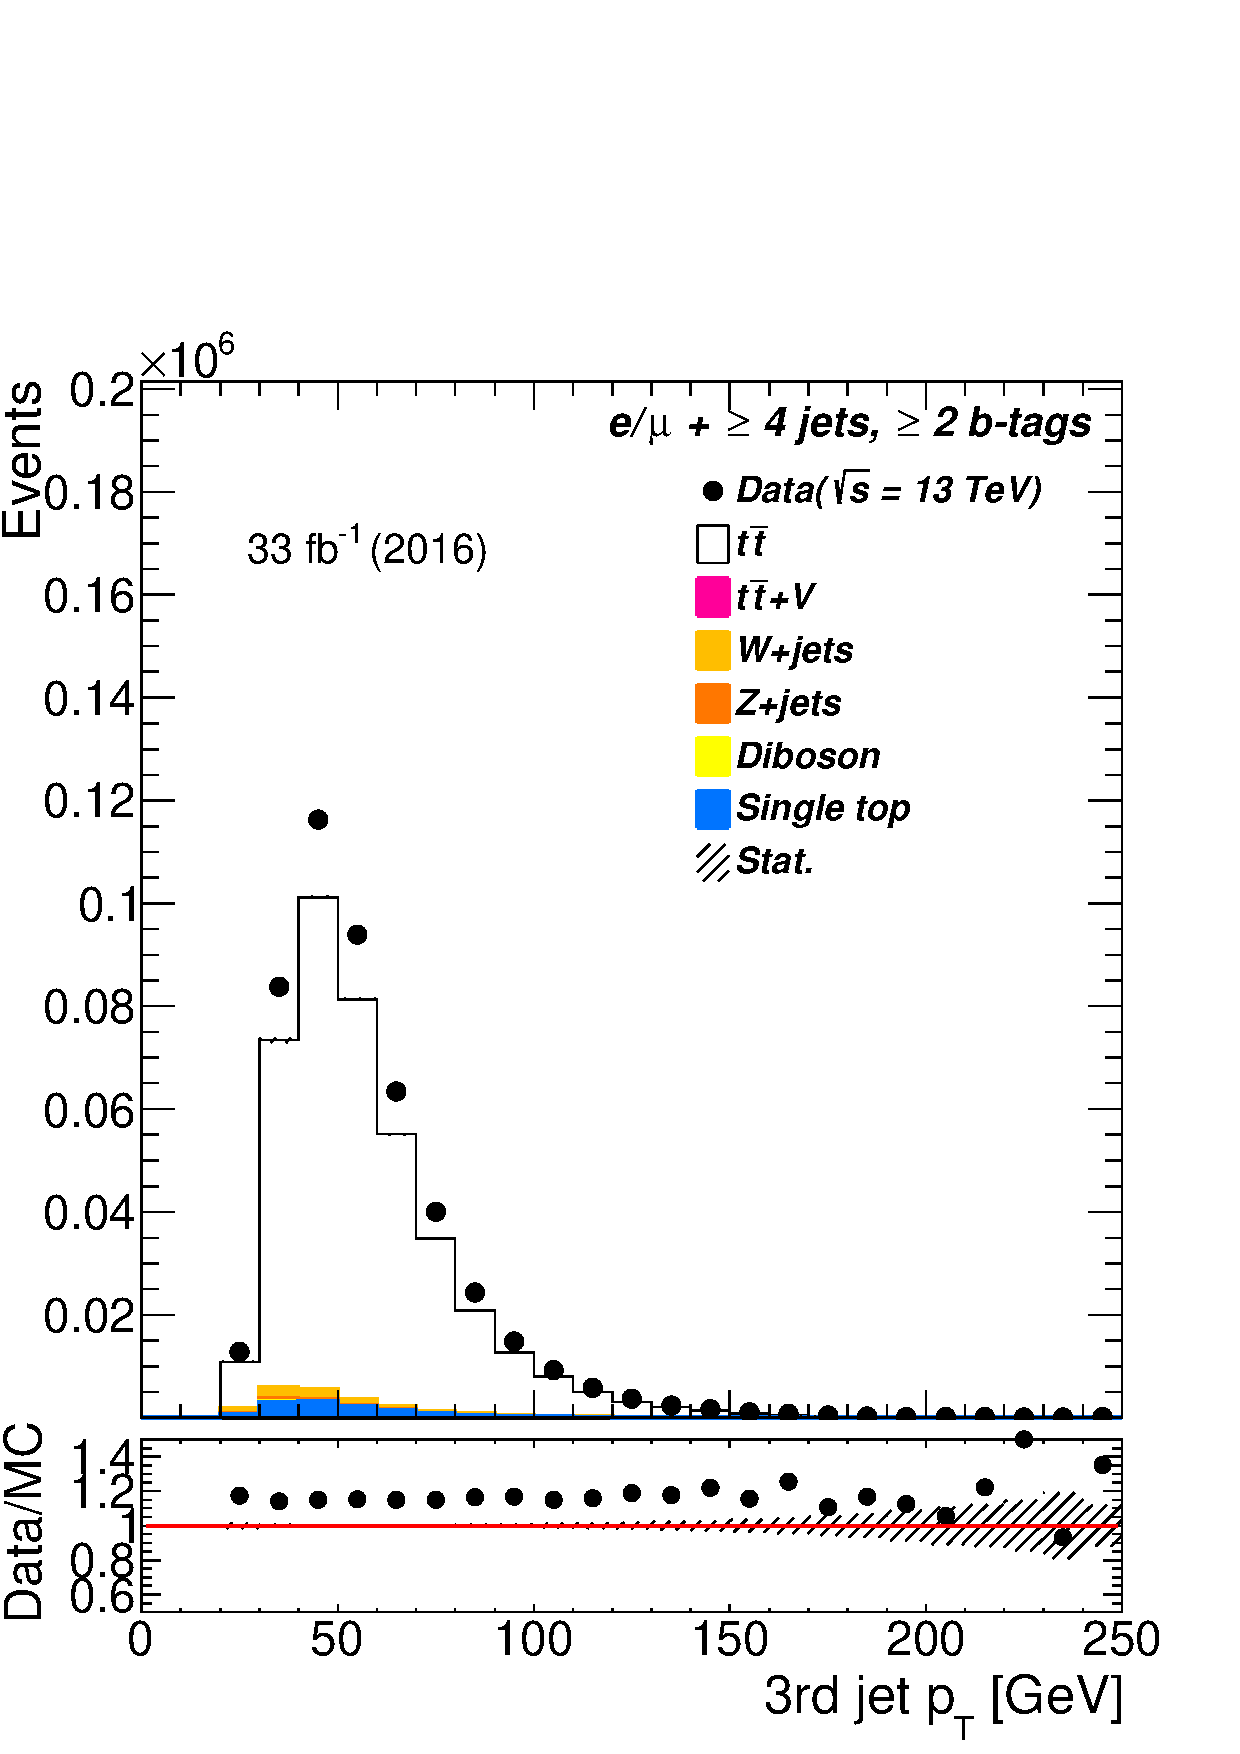
\includegraphics[width=\linewidth]{ControlPlots_emujets_2016_4incl_2incl/jet2_pt_emujets_2016.png}
		\caption{$p_T$ of the third jet.} \label{fig:Sec27}
	\end{subfigure}\hspace*{0.5cm}
	\begin{subfigure}{0.25\textwidth}
		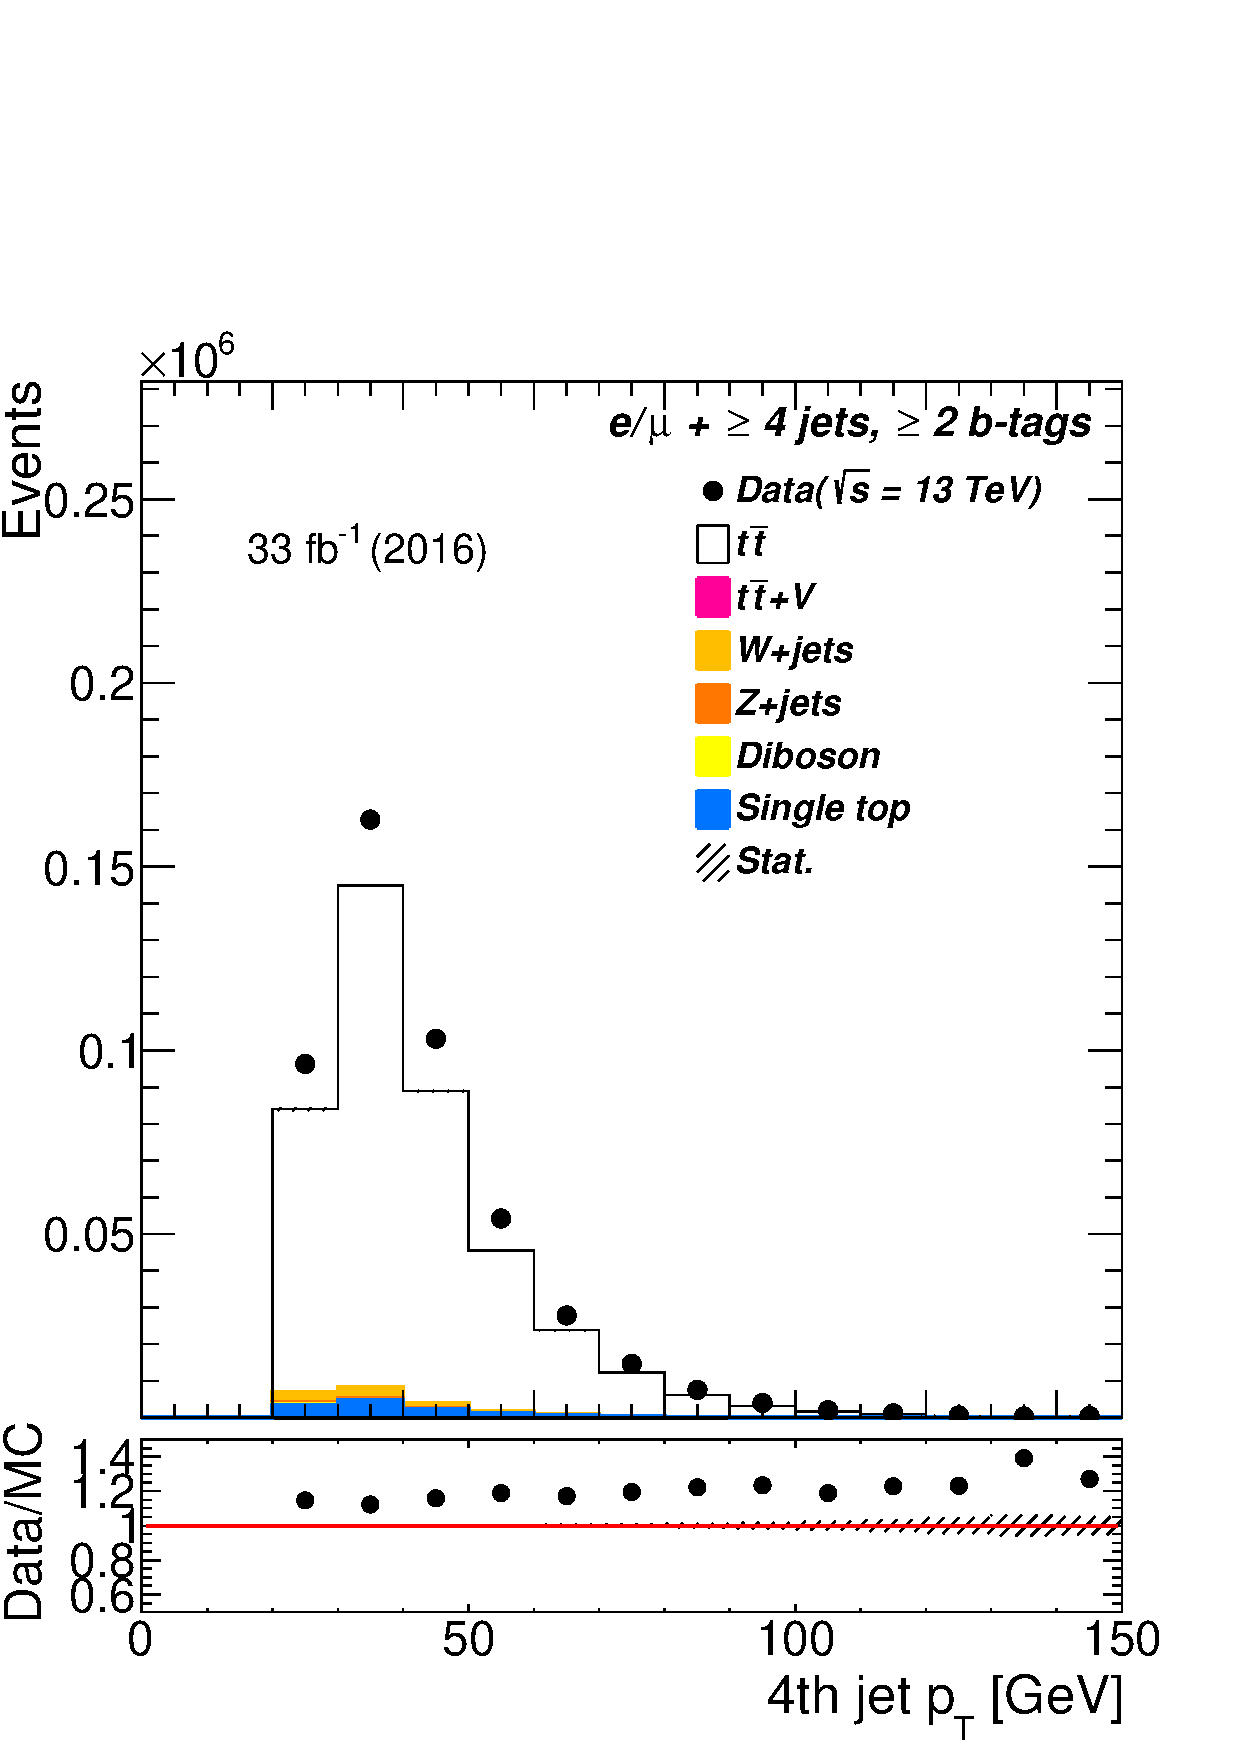
\includegraphics[width=\linewidth]{ControlPlots_emujets_2016_4incl_2incl/jet3_pt_emujets_2016.png}
		\caption{$p_T$ of the fourth jet.} \label{fig:Sec28}
	\end{subfigure}
	
	
	\caption{As in in~\cref{fig:Sel1}, transverse momentum distributions  for of the four jets, obtained for the sample with at least 4 jets and at last two $b$-tagged jets.}
	\label{fig:Sel4}
\end{figure}



\subsubsection{Global reconstructed quantities}


In the following the control distributions of the three estimators that are used in this thesis are displayed in~\cref{fig:K3,fig:K4,fig:K5}, together with further observables  reconstructed with \textsc{KLFitter}. 
All shown control distributions contain at least $4$-jets with at least two $b$-tagged jets.  The ratio plots below the histograms show the data-simulation comparison. Only the statistical uncertainties are shown and the QCD-multijet background is not included. Further reconstructed distributions can be find in~\cref{sec:app0}. 



 Despite the general slight offset of the data points with to the solid histogram lines of the simulation, the number of events for almost each simulated distribution, remains consistent with the observed numbers in data.

 For the hadronic top $p_T$ spectrum~\cref{fig:K10}, however, the distribution is softer in data than predicted by the simulation. This issue has also been discovered by the 8~TeV analysis, where it was studied extensively with the result that it will only affect the measurement, if the observed deviations are not covered by the systematic uncertainties~\cite{ATLAS-CONF-2017-071}. Since this is not the case for the 8~TeV measurement, it is assumed that this observation will also not affect the analysis presented here. Further investigations are needed when all  uncertainties are included in the analysis. 




 


\begin{figure} % "[t!]" placement specifier just for this example
	\centering




	\begin{subfigure}{0.25\textwidth}
		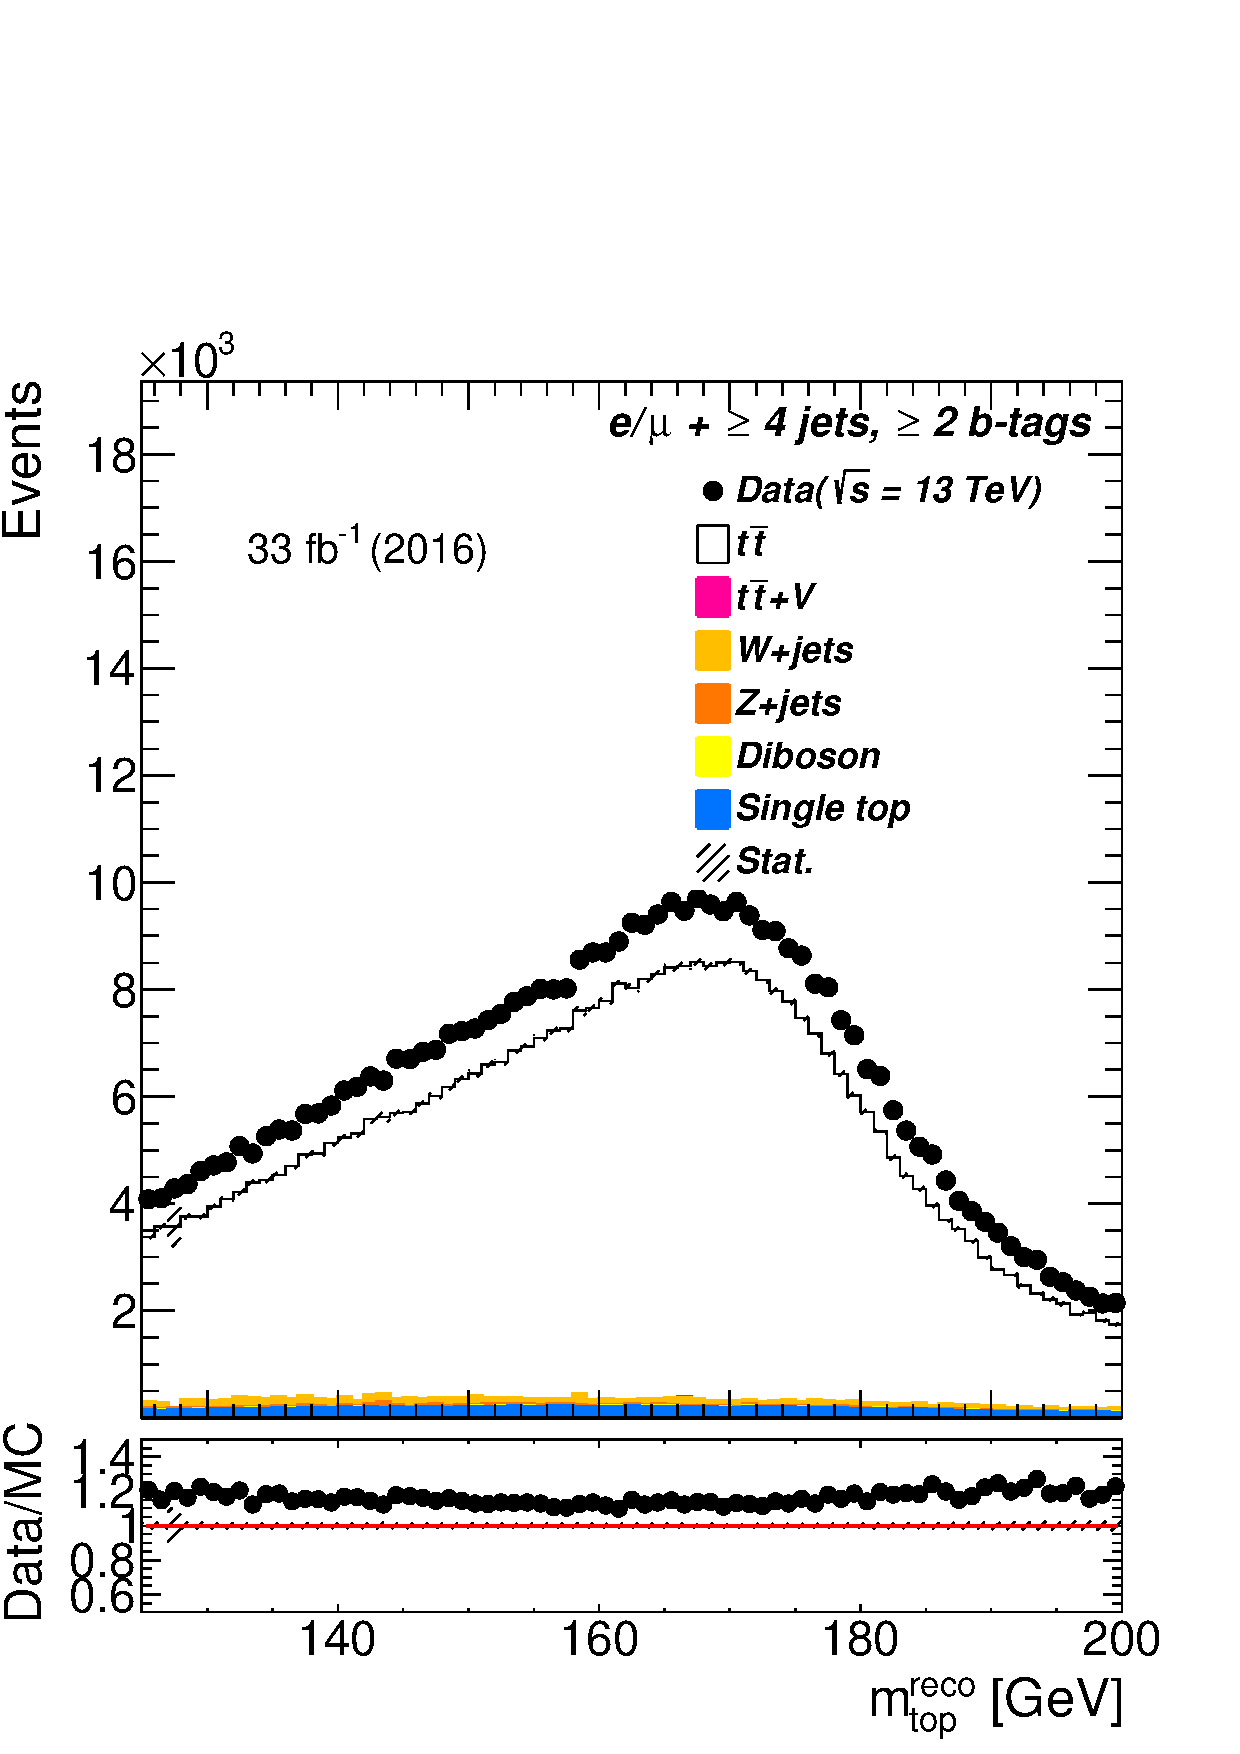
\includegraphics[width=\linewidth]{ControlPlots_emujets_2016_4incl_2incl//klf_window_mtop_reco_emujets_2016.png}
		\caption{Reconstructed hadronic top-quark mass $m_{top}^{reco}$.} \label{fig:K3}
	\end{subfigure}	\hspace*{0.5cm}
	\begin{subfigure}{0.25\textwidth}
		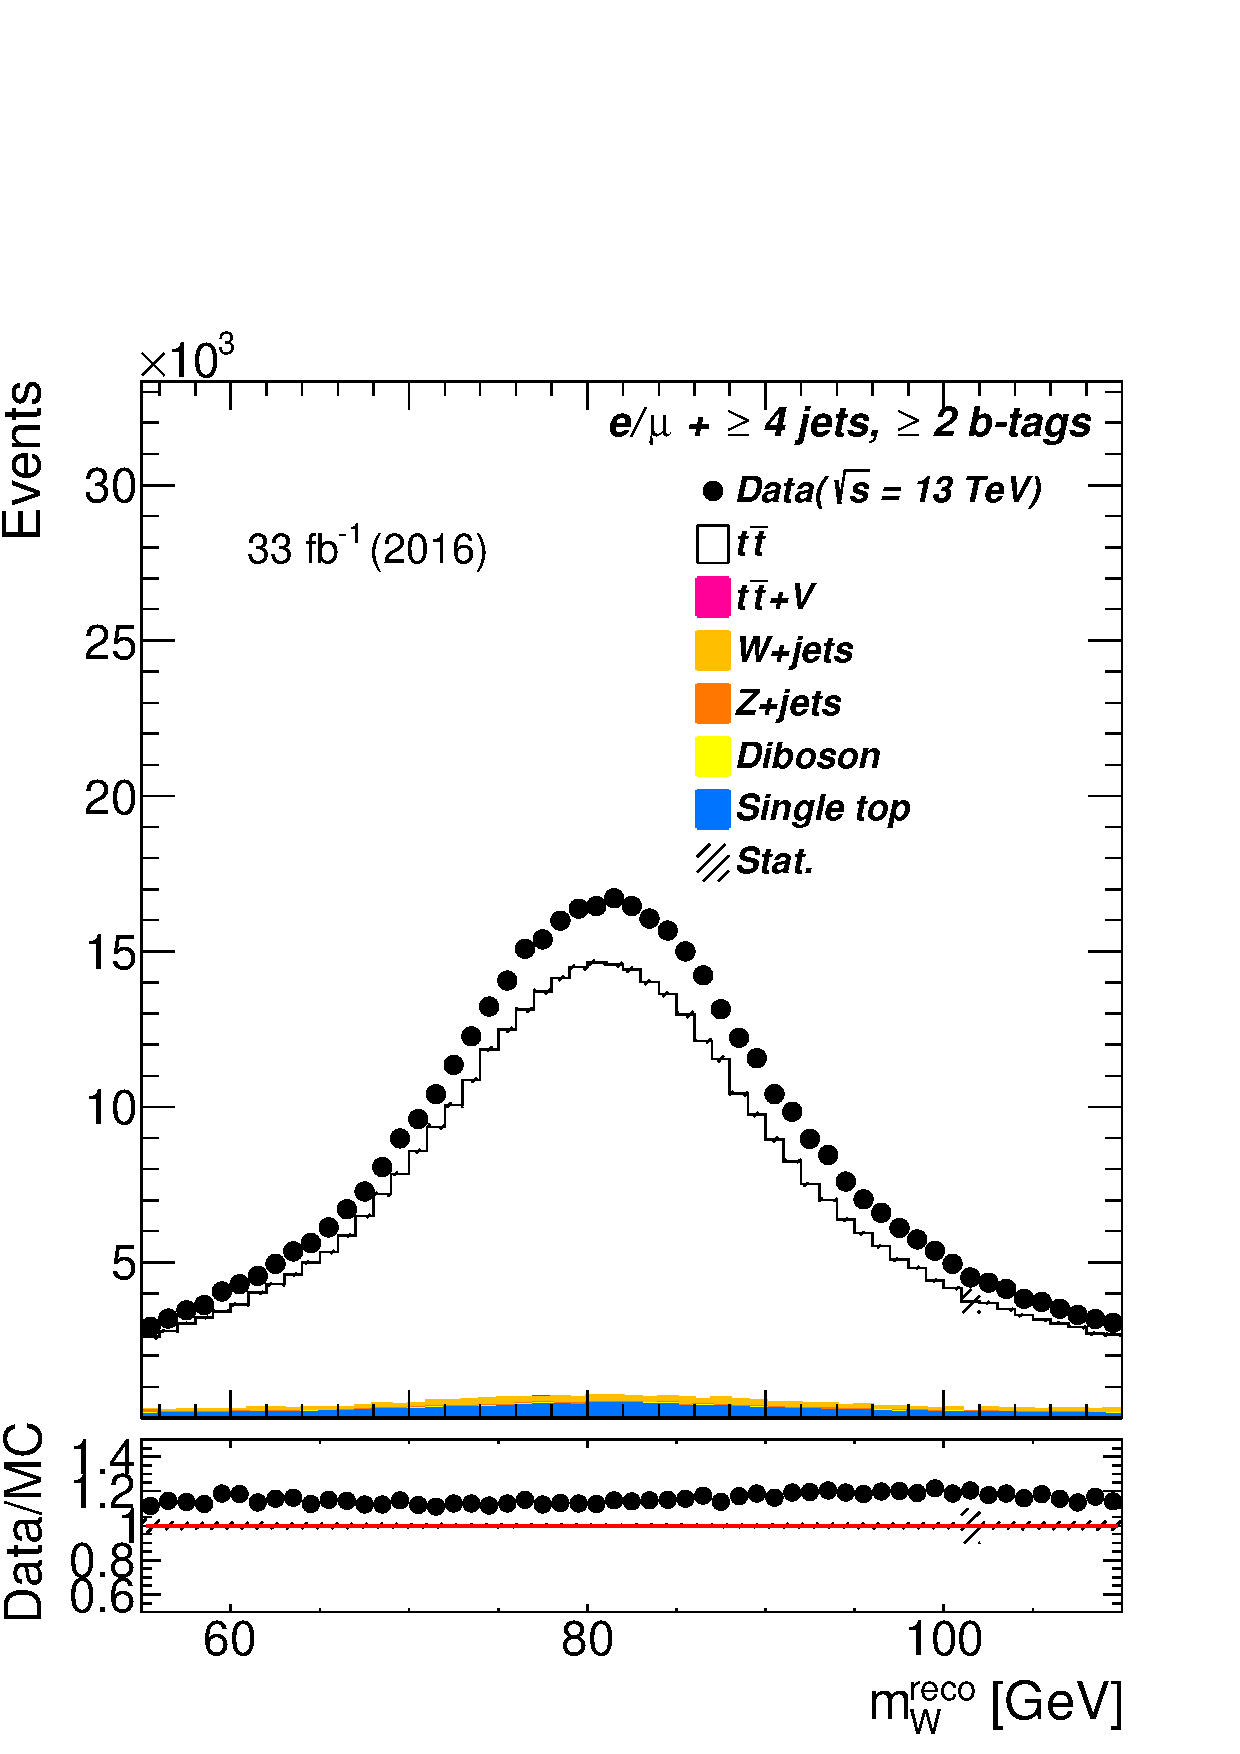
\includegraphics[width=\linewidth]{ControlPlots_emujets_2016_4incl_2incl/klf_window_mw_reco_emujets_2016.pdf}
		\caption{Reconstructed hadronic top-quark mass $m_{W}^{reco}$.} \label{fig:K4}
	\end{subfigure}	\hspace*{0.5cm}	
	\begin{subfigure}{0.25\textwidth}
		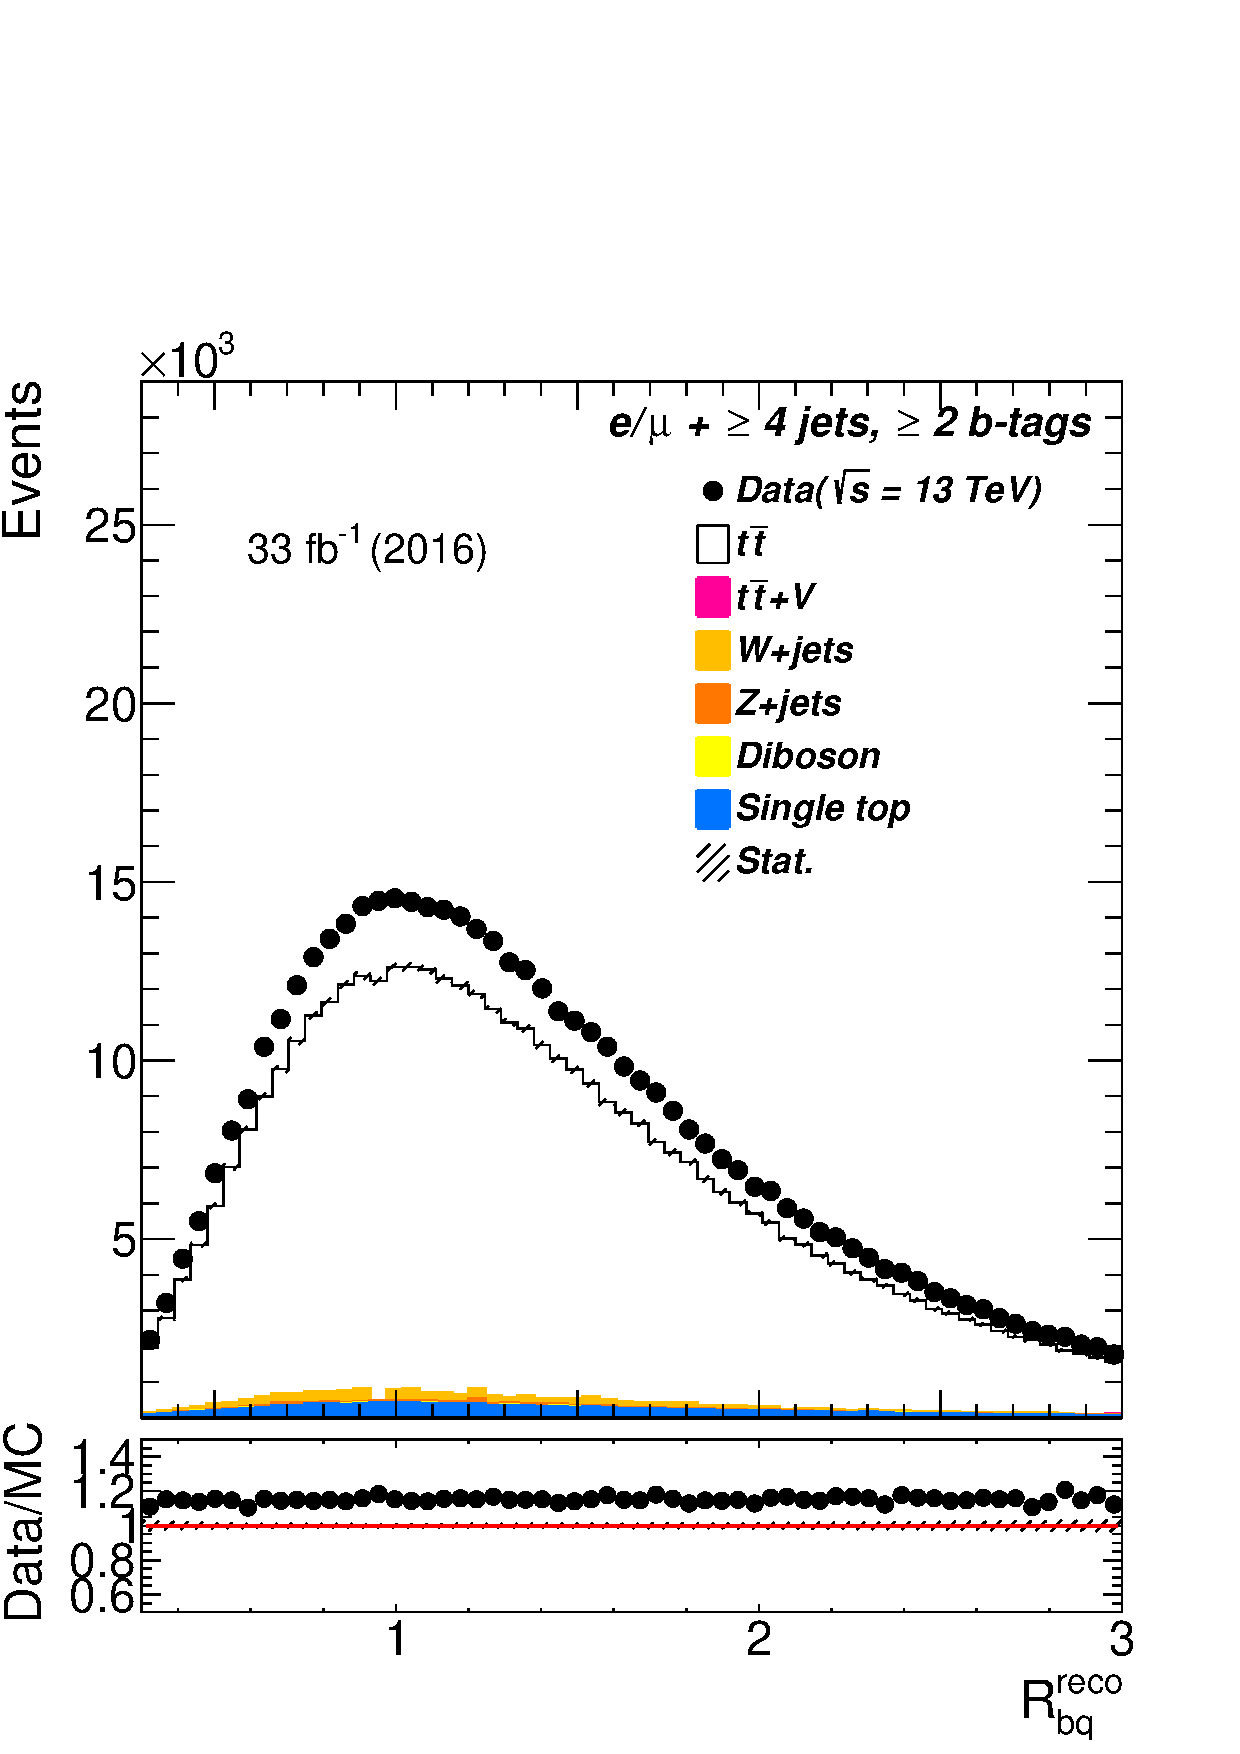
\includegraphics[width=\linewidth]{ControlPlots_emujets_2016_4incl_2incl/klf_window_rbq_reco_emujets_2016.png}
		\caption{Reconstructed $p_T$ ratio $R_{bq}^{reco}$.} \label{fig:K5}
	\end{subfigure}




\begin{subfigure}{0.25\textwidth}
	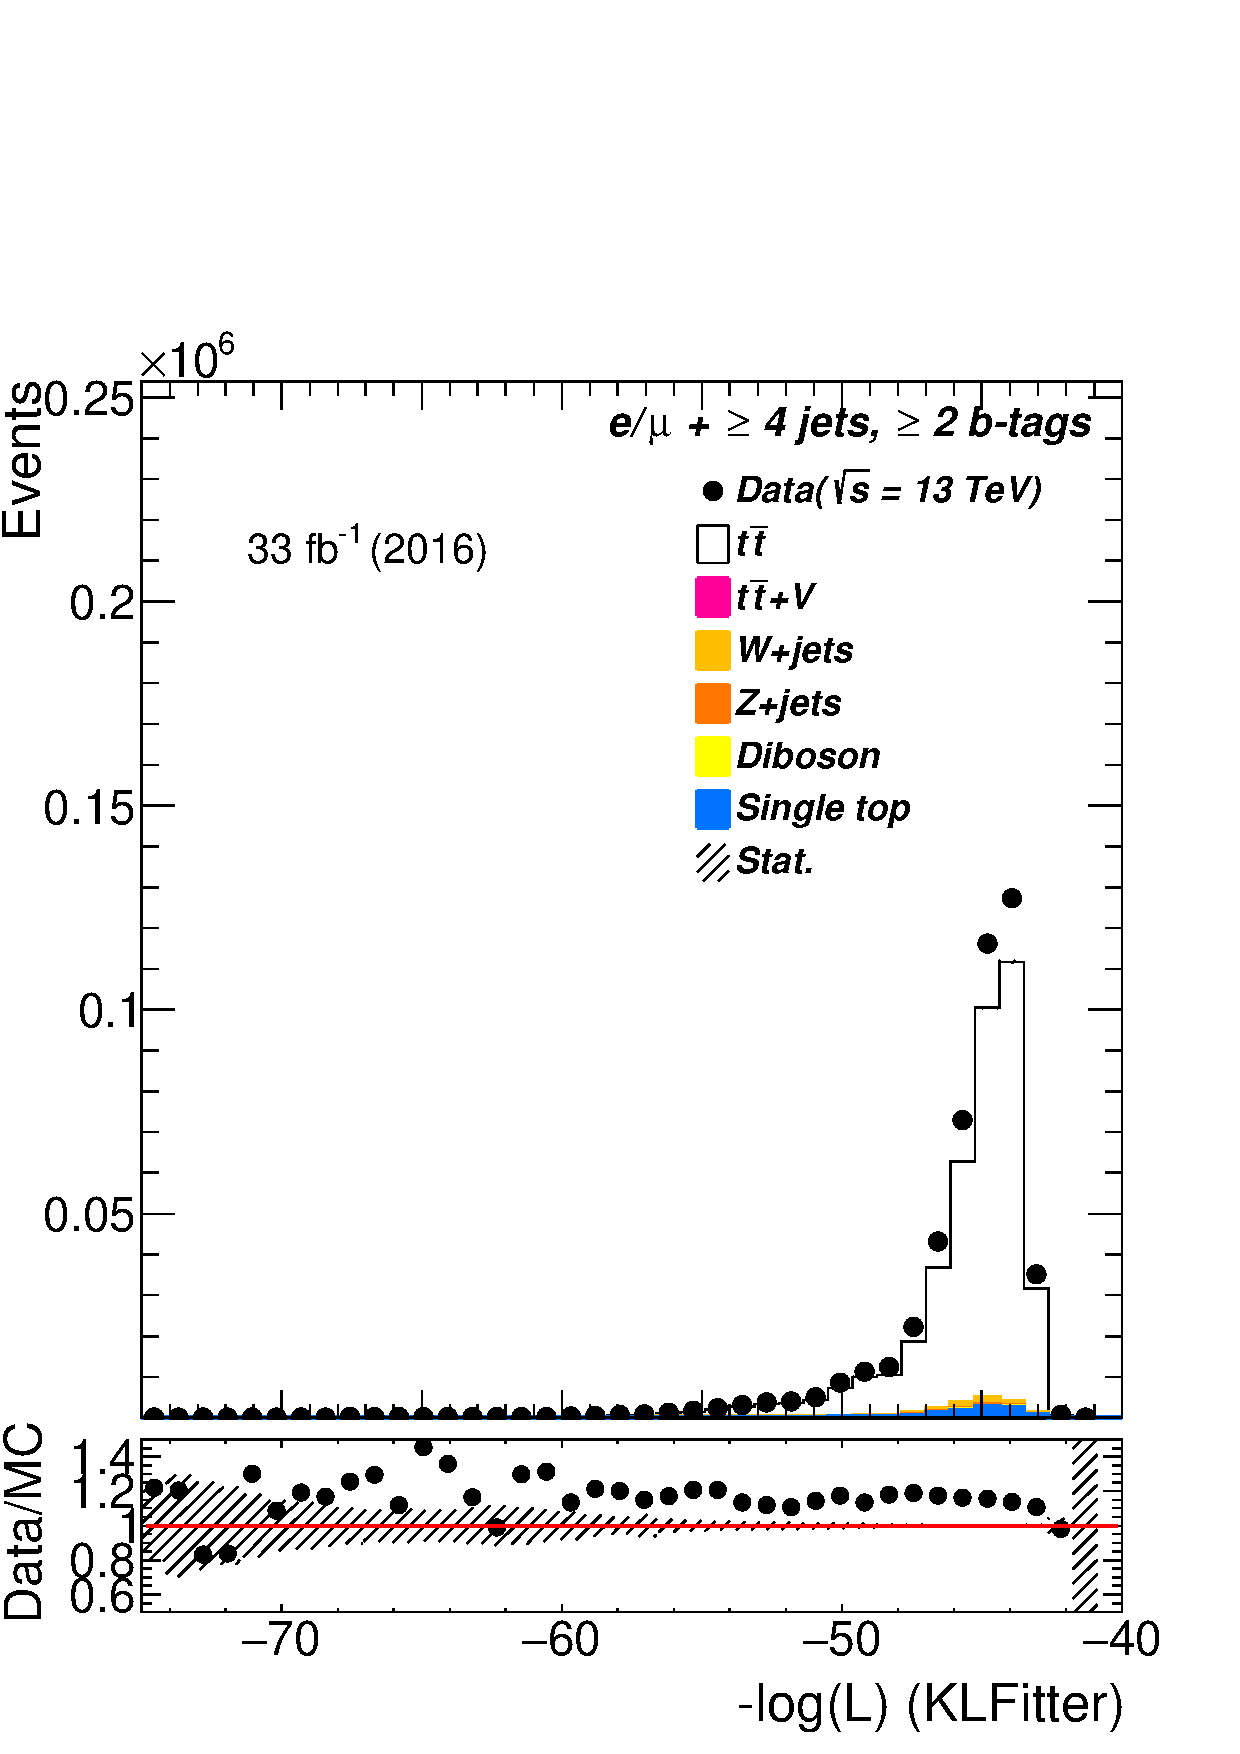
\includegraphics[width=\linewidth]{ControlPlots_emujets_2016_4incl_2incl/klf_LL_emujets_2016.png}
	\caption{The kinematic logarithmic \textsc{KLFitter} likelihood function.} \label{fig:K2}
\end{subfigure}\hspace*{0.5cm}	
	\begin{subfigure}{0.25\textwidth}
	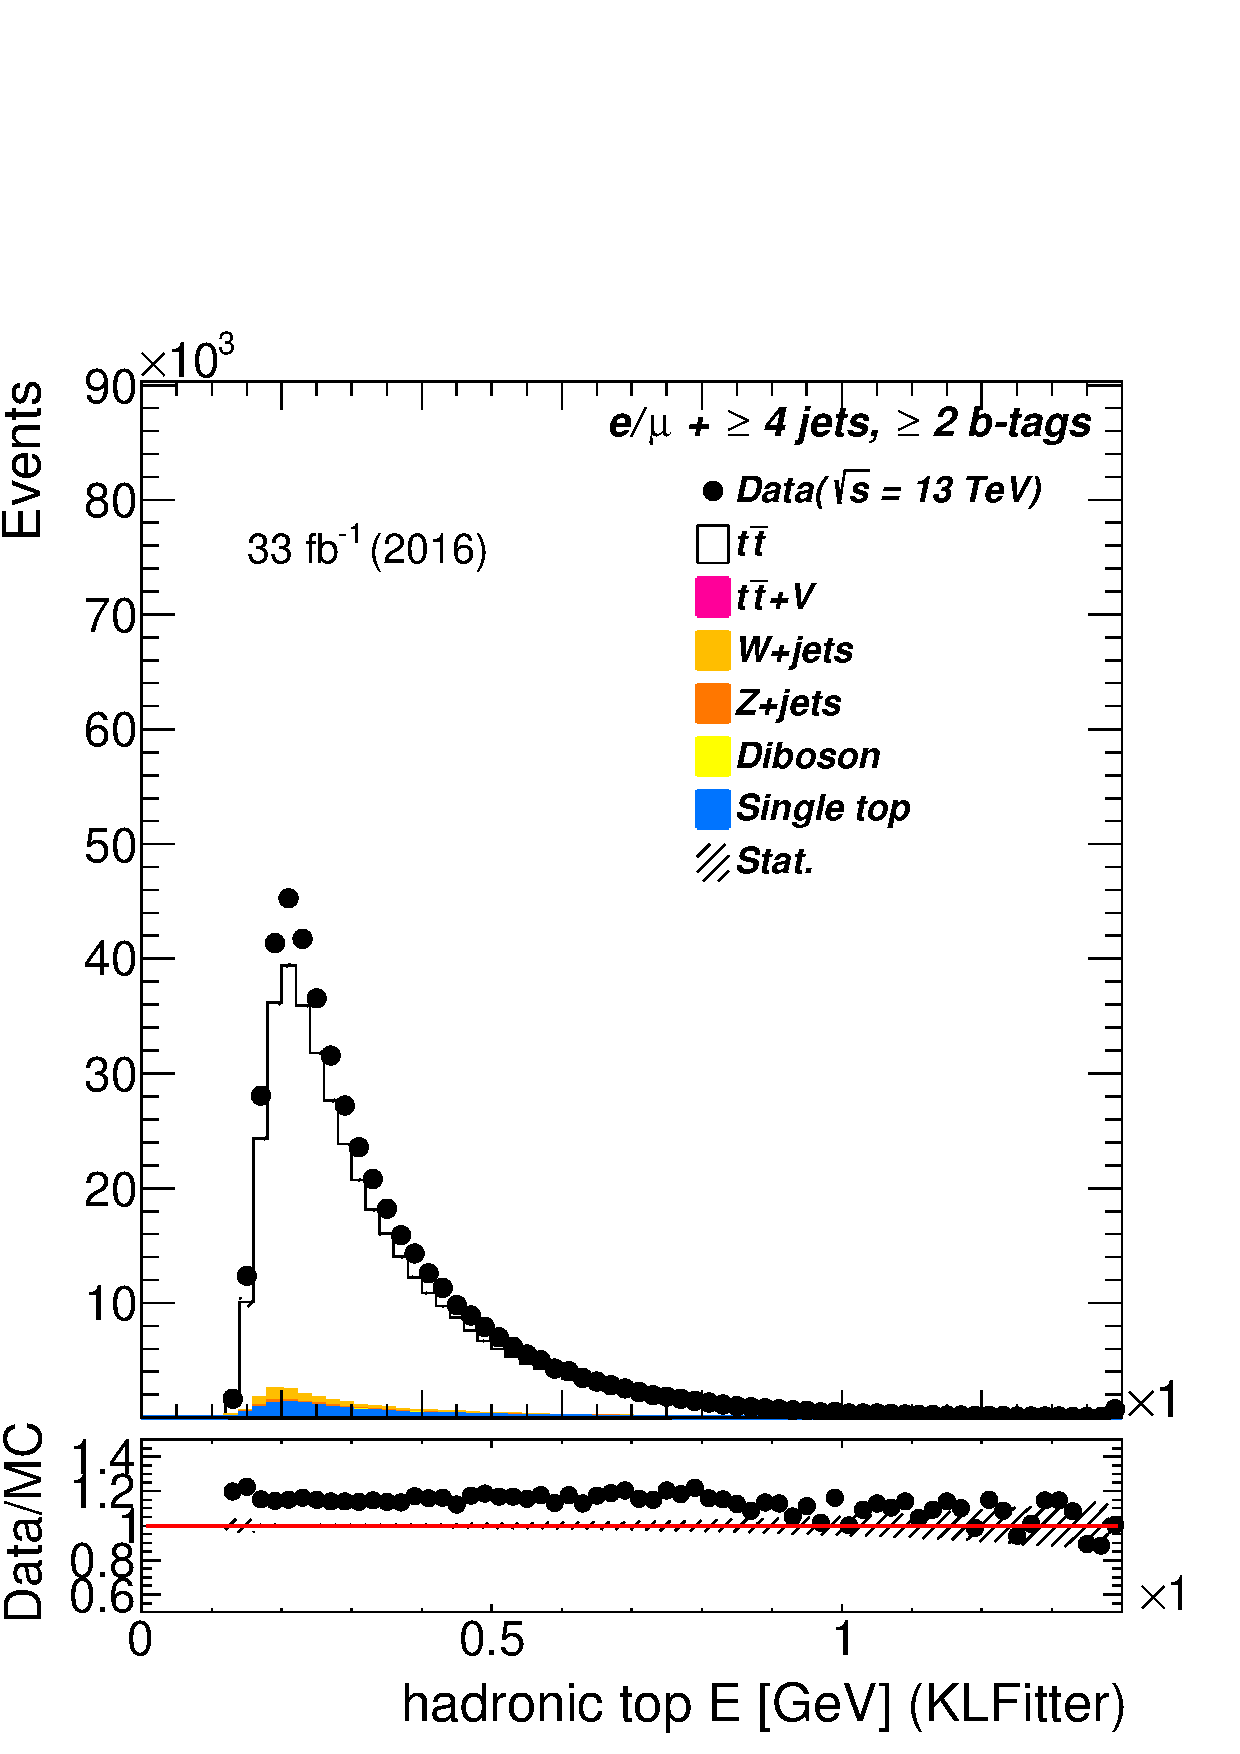
\includegraphics[width=\linewidth]{ControlPlots_emujets_2016_4incl_2incl/klf_topHad_E_emujets_2016.png}
	\caption{Energy of the hadronic top quark.} \label{fig:K7}
\end{subfigure}
\hspace*{0.5cm}
\begin{subfigure}{0.25\textwidth}
	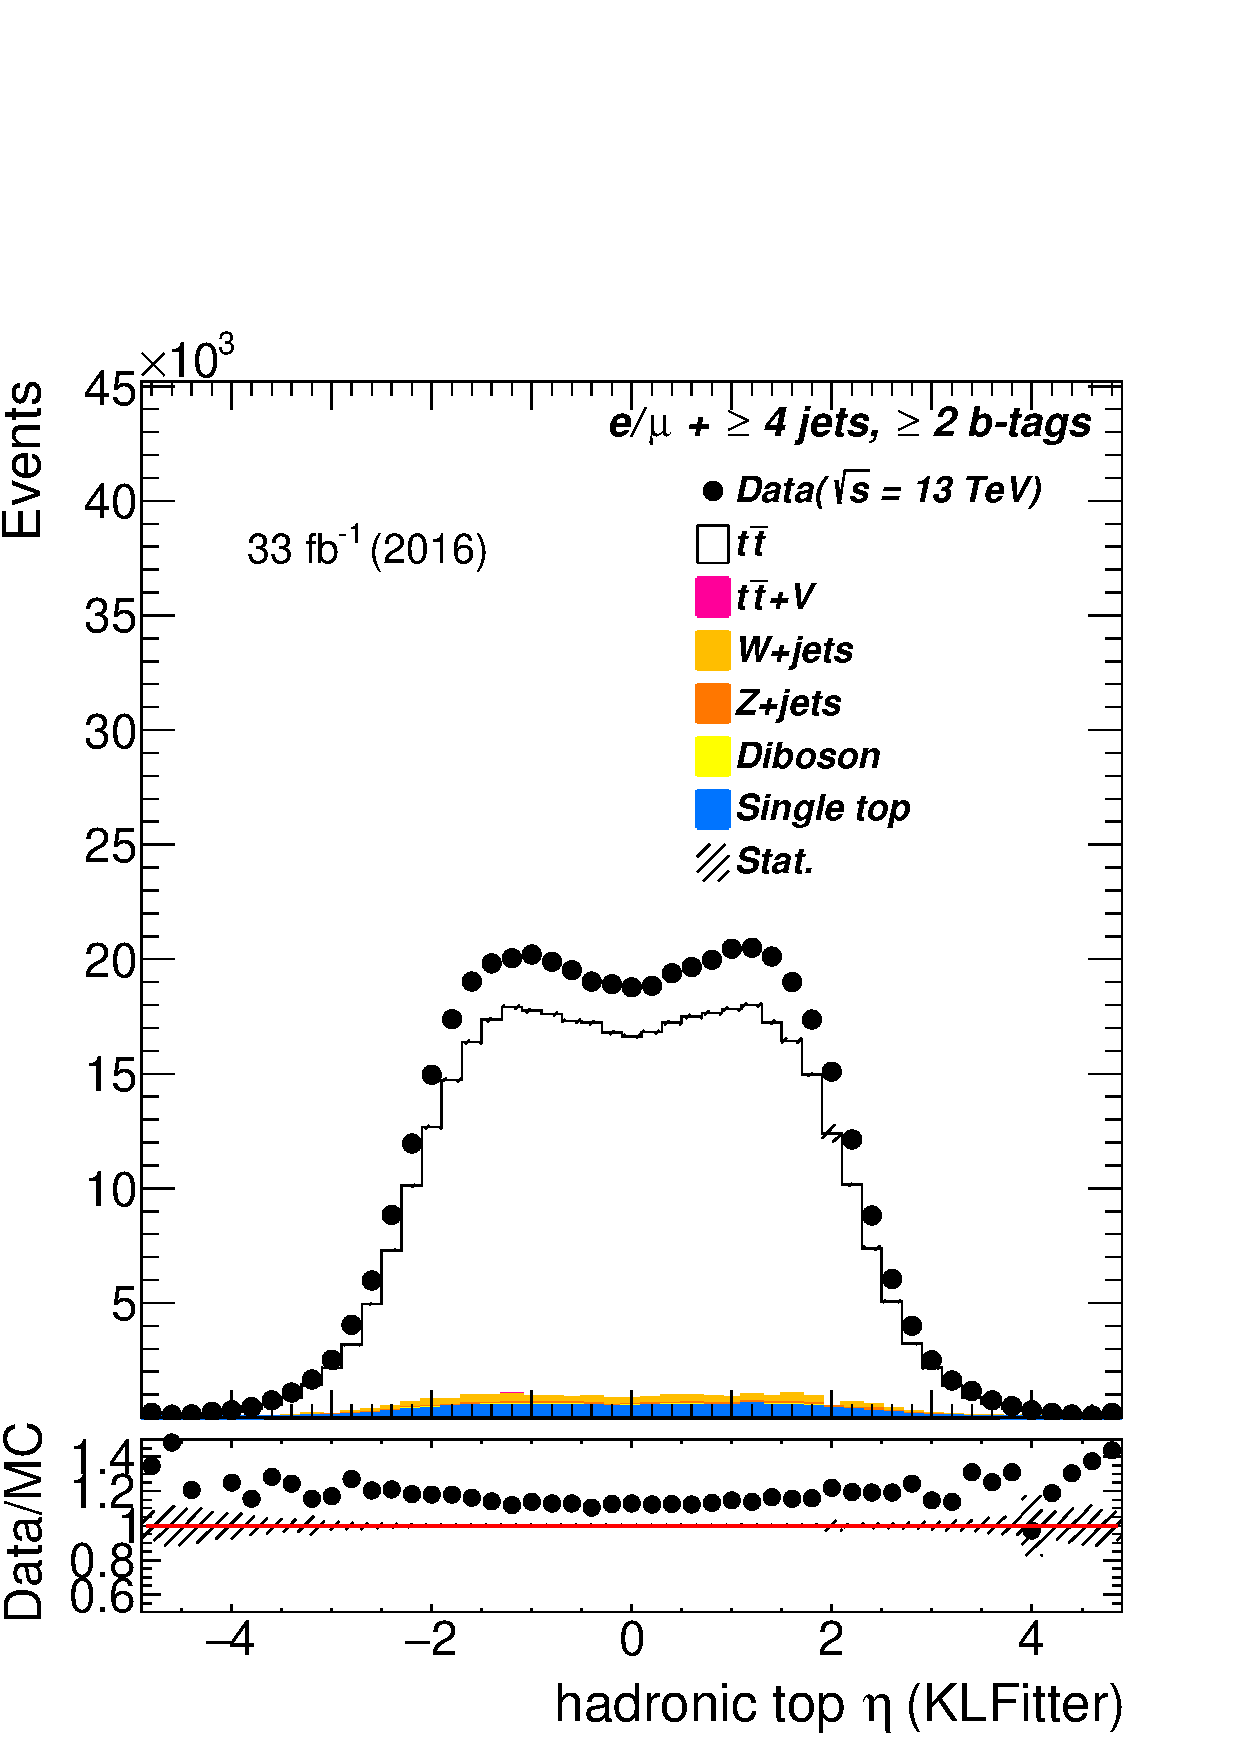
\includegraphics[width=\linewidth]{ControlPlots_emujets_2016_4incl_2incl/klf_topHad_eta_emujets_2016.png}
	\caption{$\eta$ of the hadronic top quark.} \label{fig:K8}
\end{subfigure}



	\begin{subfigure}{0.25\textwidth}
	\includegraphics[width=\linewidth]{ControlPlots_emujets_2016_4incl_2incl/klf_topHad_phi_emujets_2016.png}
	\caption{$\phi$ of the hadronic top quark.} \label{fig:K9}
\end{subfigure}	
\hspace*{0.5cm}	
\begin{subfigure}{0.25\textwidth}
	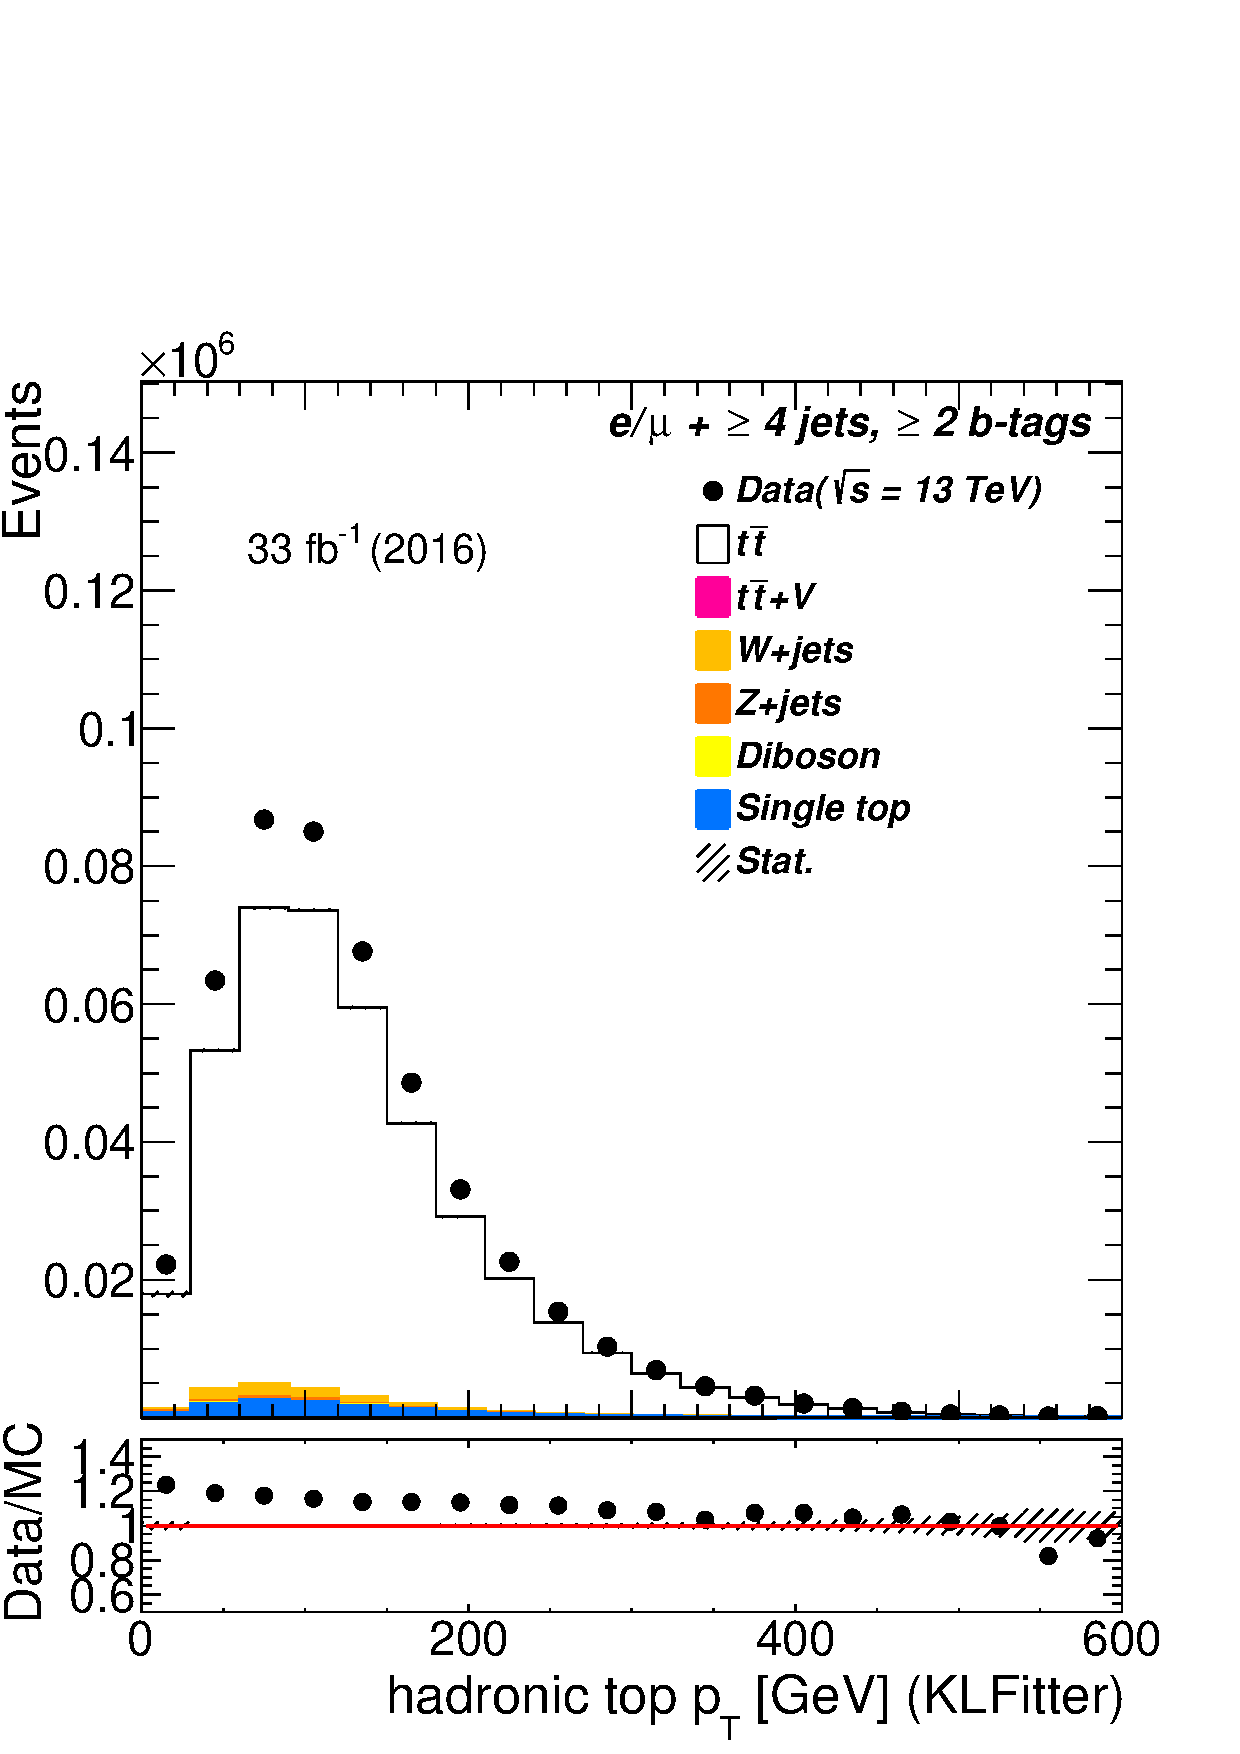
\includegraphics[width=\linewidth]{ControlPlots_emujets_2016_4incl_2incl/klf_topHad_pt_emujets_2016.png}
	\caption{Transverse momentum of the hadronic top quark.} \label{fig:K10}
\end{subfigure}\hspace*{0.5cm}
\begin{subfigure}{0.25\textwidth}
	\includegraphics[width=\linewidth]{ControlPlots_emujets_2016_4incl_2incl/klf_topLEP_E_emujets_2016.png}
	\caption{Energy of the leptonic top quark.} \label{fig:K11}
\end{subfigure}

\caption{Reconstructed global quantities, obtained with \textsc{KLFitter}. The black points represent the data, while the simulation is denoted by the solid histogram. The simulation of the different background processes are also shown by the coloured histograms. The data-simulation agreement is shown by the lower plot. Only statical errors are considered and the QCD-multijet background  is missing. The log-likelihood distribution is used by \textsc{KLFitter}, to obtain the best jet-patron assignment. The hadronic top-quark and  $W$-boson mass, as well as $R_{bq}^{reco}$ are very important quantities, which are generated from the event kinematics. If not mentioned different, the term hadronic or leptoinc, refer to the corresponding decay of the top-quark pair.}\label{klf100}
\end{figure}	



\begin{figure} % "[t!]" placement specifier just for this example
	\centering

	\begin{subfigure}{0.25\textwidth}
		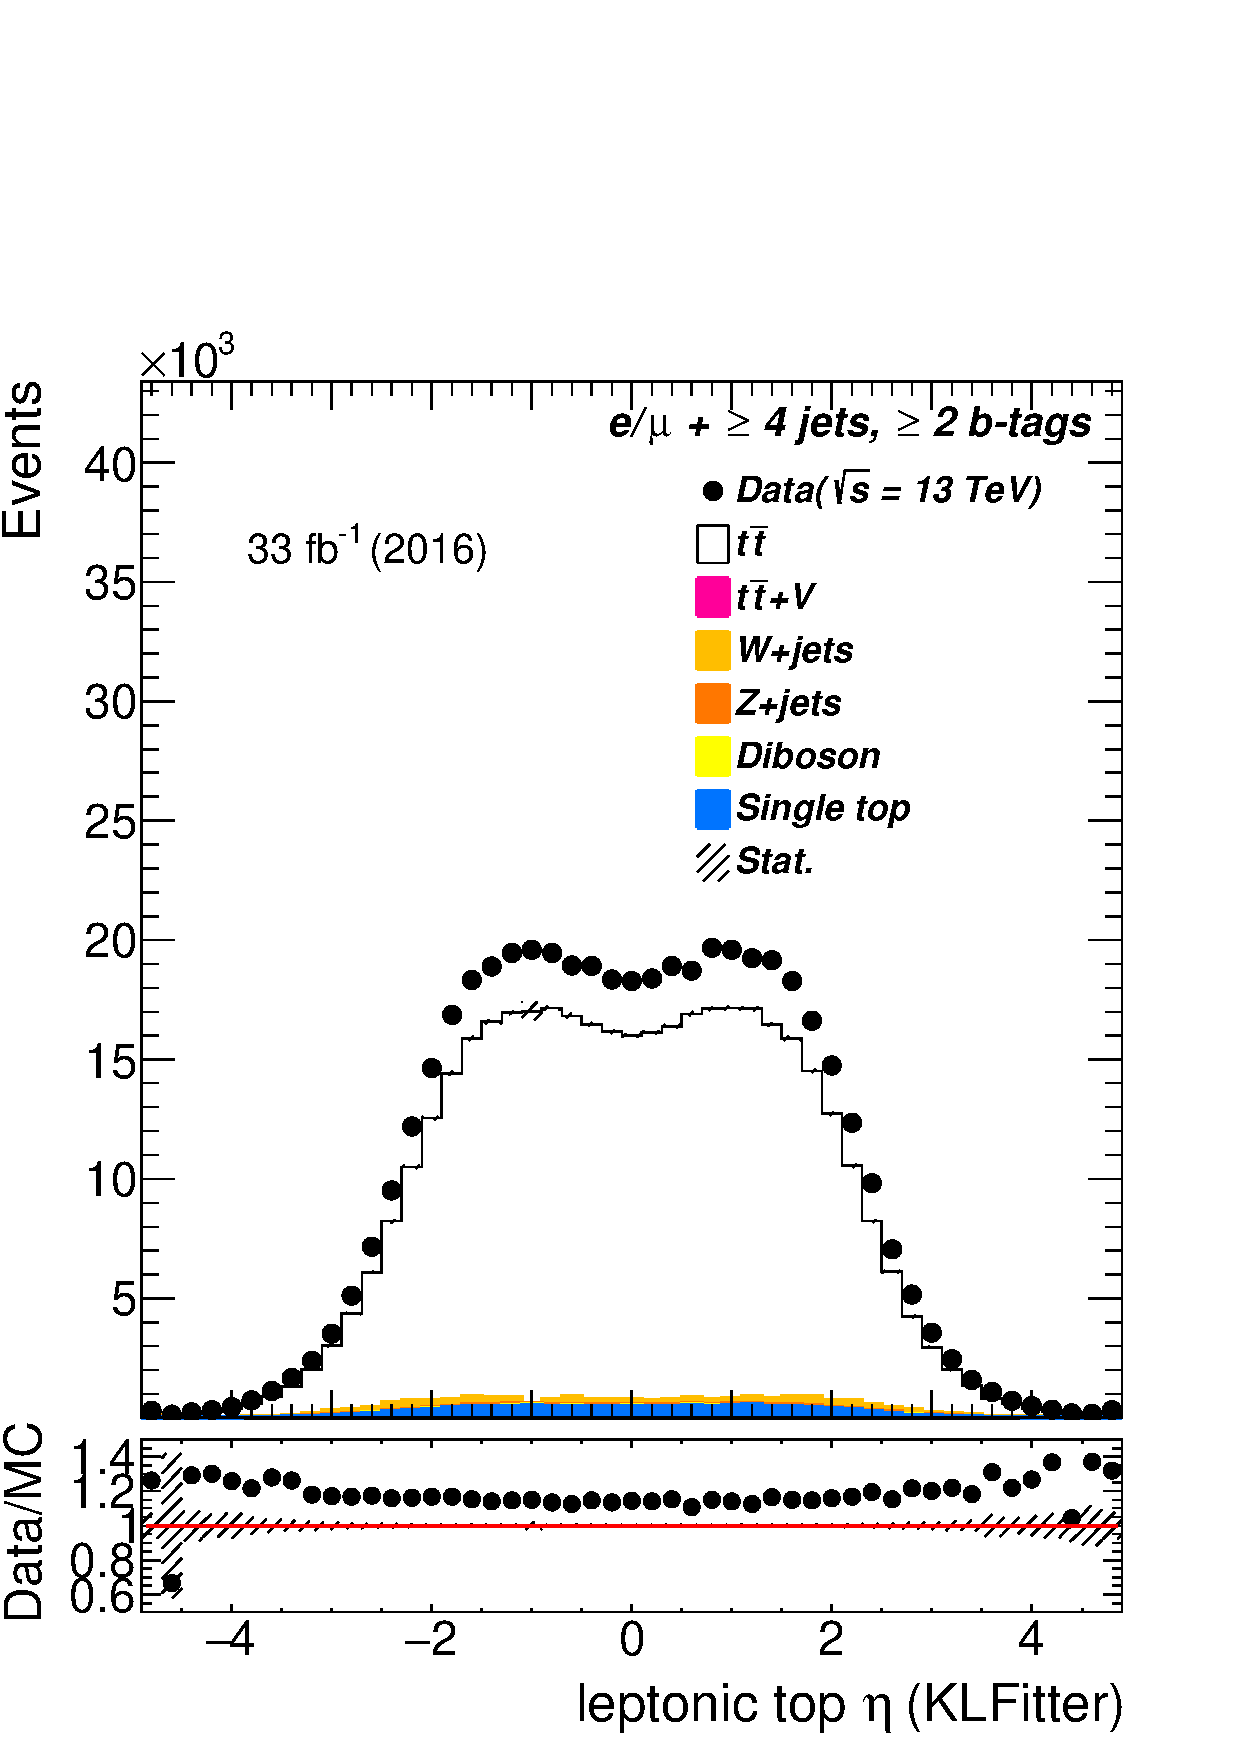
\includegraphics[width=\linewidth]{ControlPlots_emujets_2016_4incl_2incl/klf_topLep_eta_emujets_2016.png}
		\caption{$\eta$ of the leptonic top quark.} \label{fig:K12}
	\end{subfigure}	\hspace*{0.5cm}
	\begin{subfigure}{0.25\textwidth}
	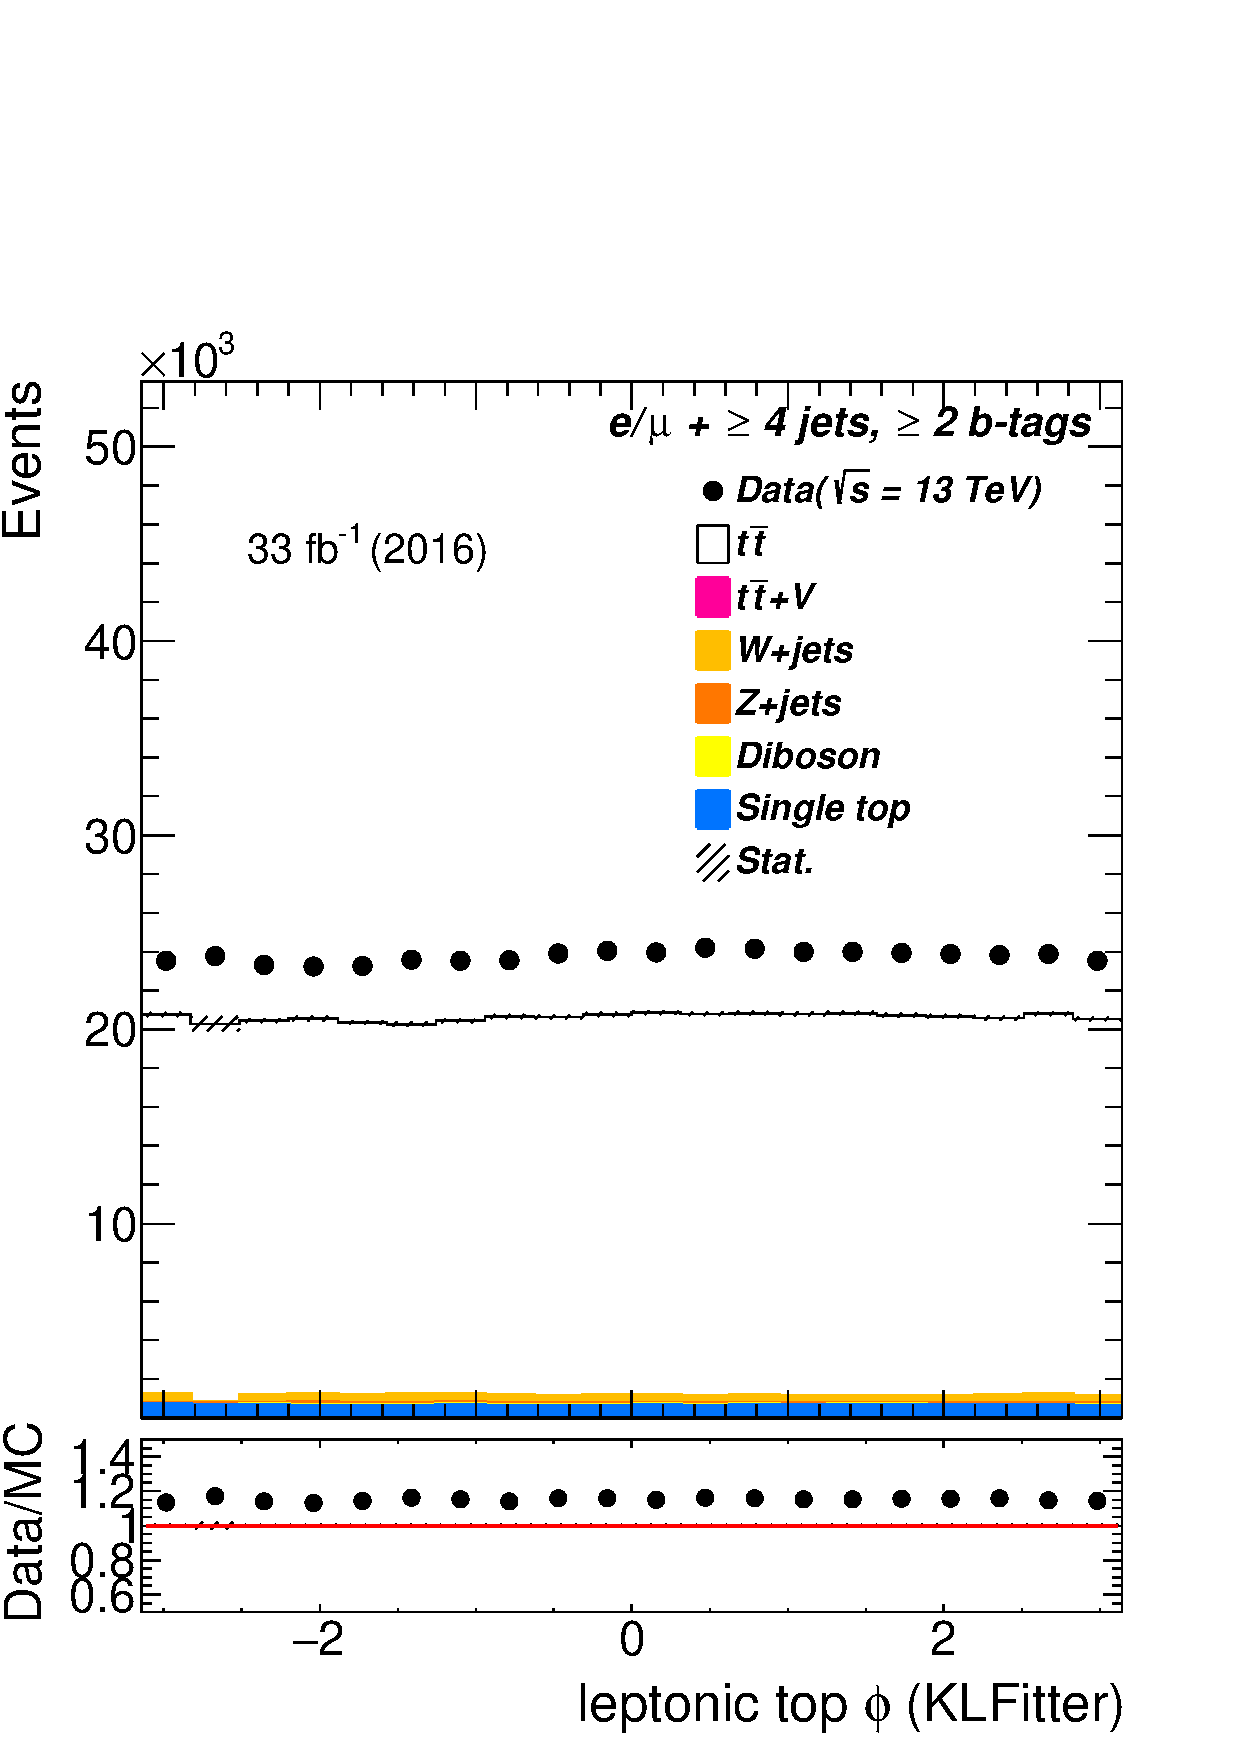
\includegraphics[width=\linewidth]{ControlPlots_emujets_2016_4incl_2incl/klf_topLep_phi_emujets_2016.png}
	\caption{$\phi$ of the leptonic top quark.} \label{fig:K13}
\end{subfigure}
\hspace*{0.5cm}
\begin{subfigure}{0.25\textwidth}
	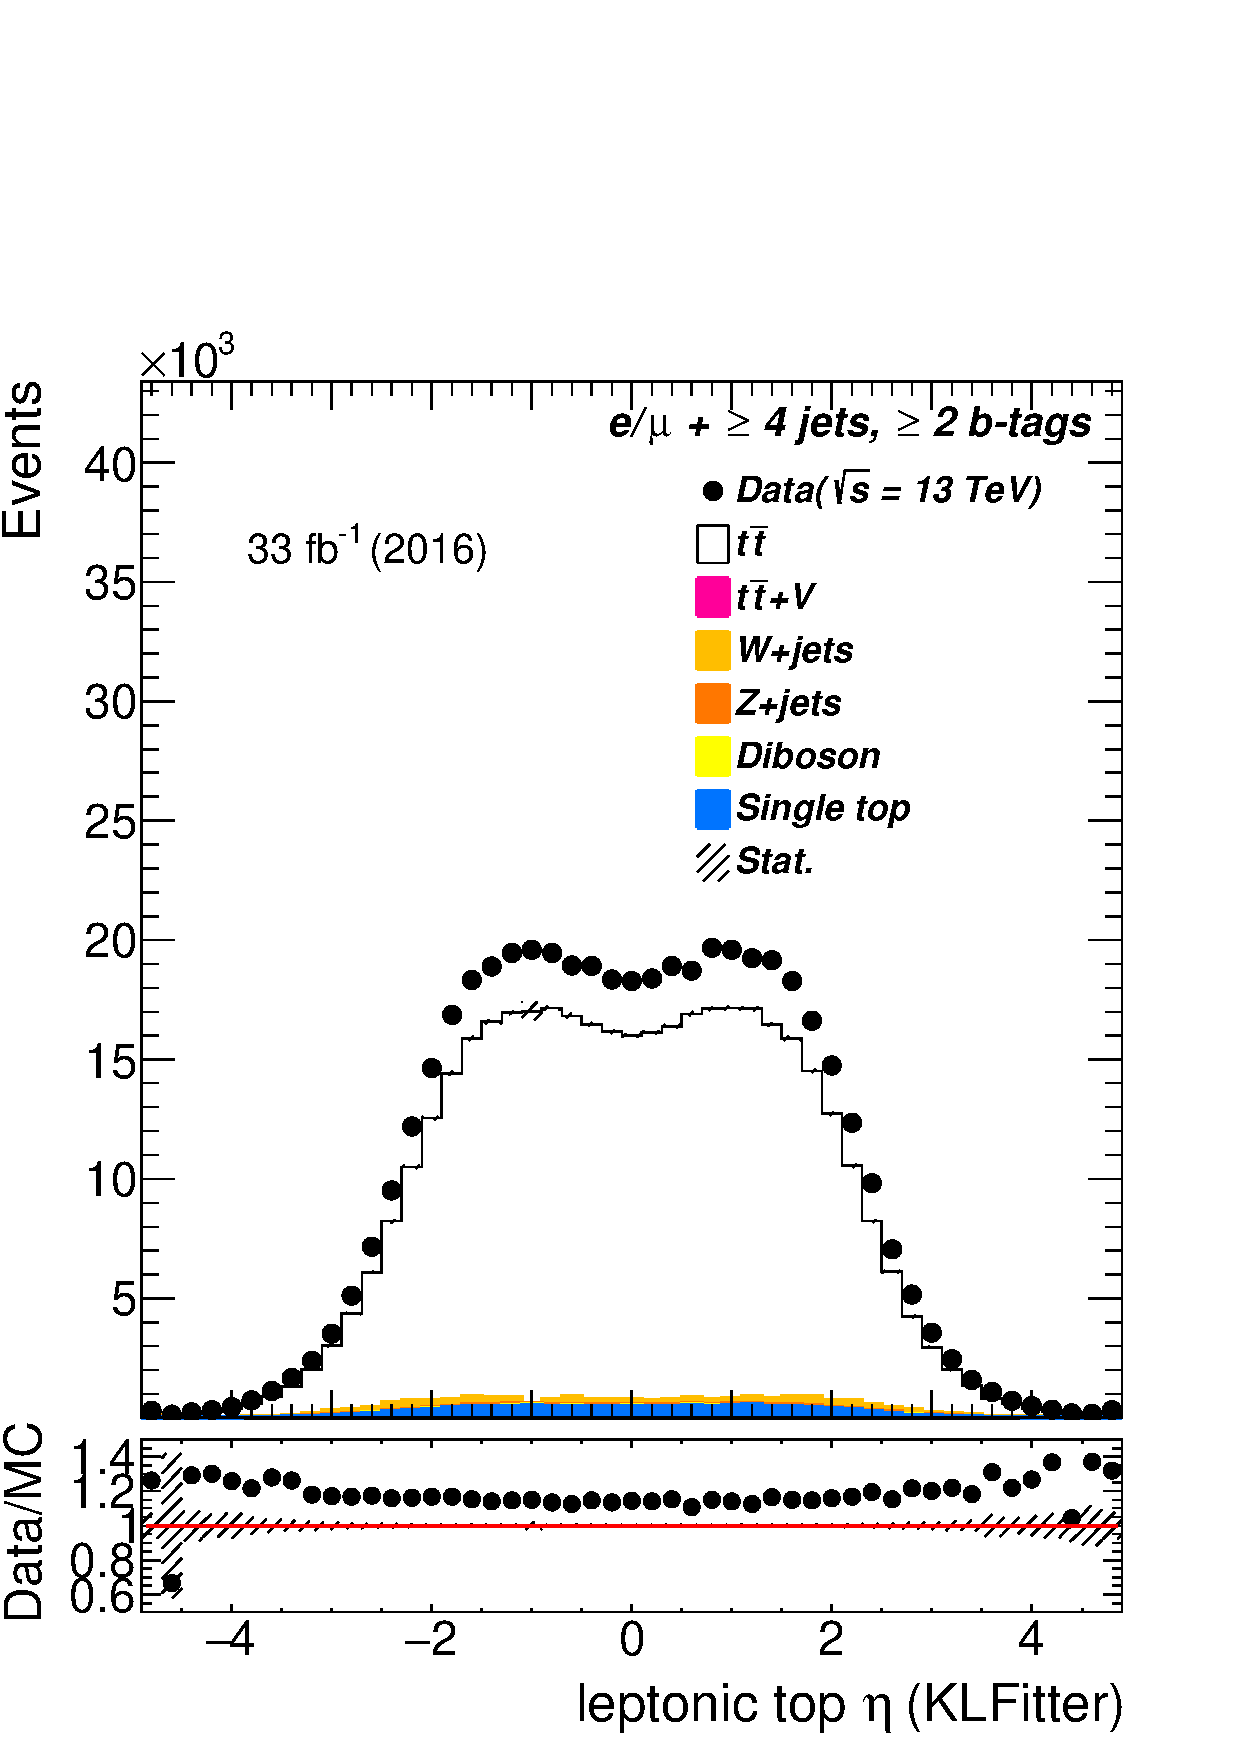
\includegraphics[width=\linewidth]{ControlPlots_emujets_2016_4incl_2incl/klf_topLep_eta_emujets_2016.png}
	\caption{$\eta$ of the leptonic top-quark.} \label{fig:K14}
\end{subfigure}



	
	
	\begin{subfigure}{0.25\textwidth}
		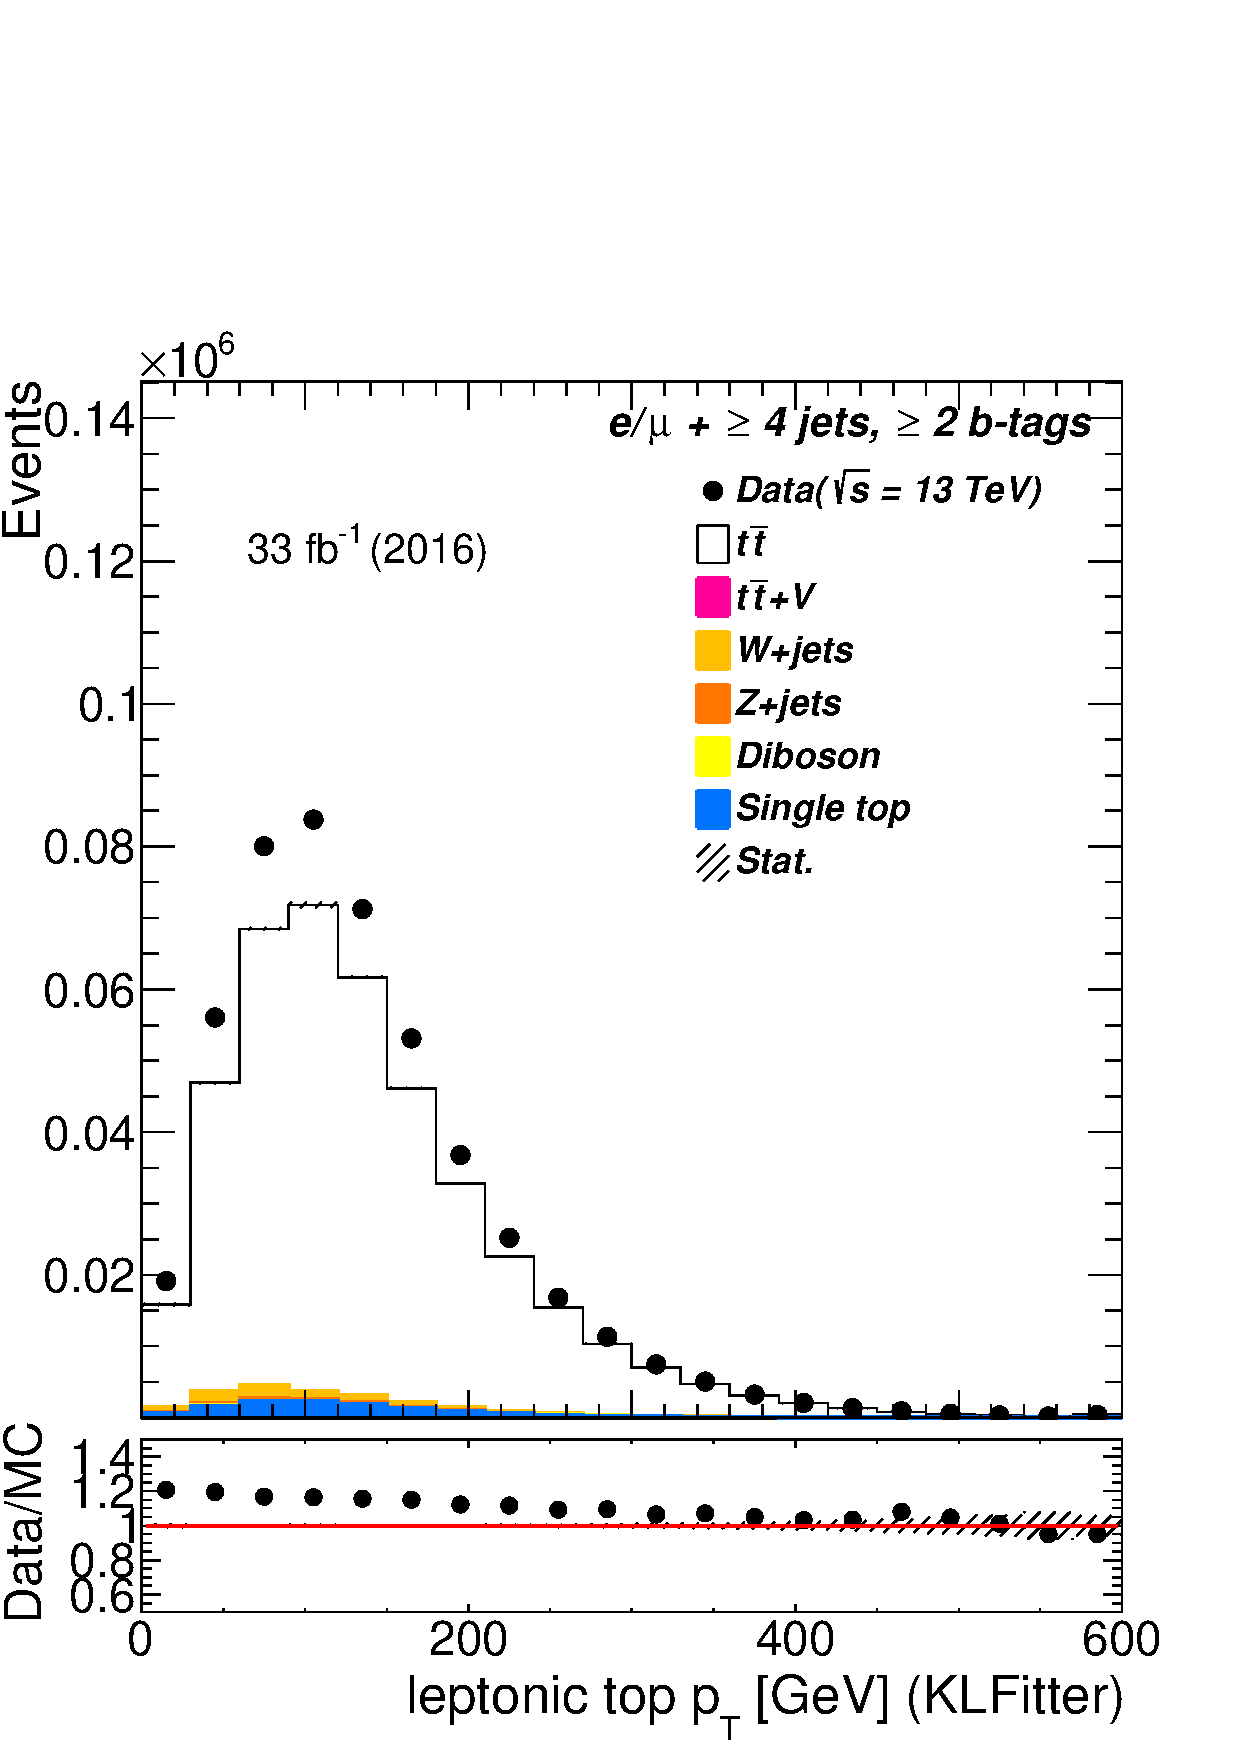
\includegraphics[width=\linewidth]{ControlPlots_emujets_2016_4incl_2incl/klf_topLep_pt_emujets_2016.png}
		\caption{Transverse momentum of the leptonic quark.} \label{fig:K15}
	\end{subfigure}	\hspace*{0.5cm}
	\begin{subfigure}{0.25\textwidth}
		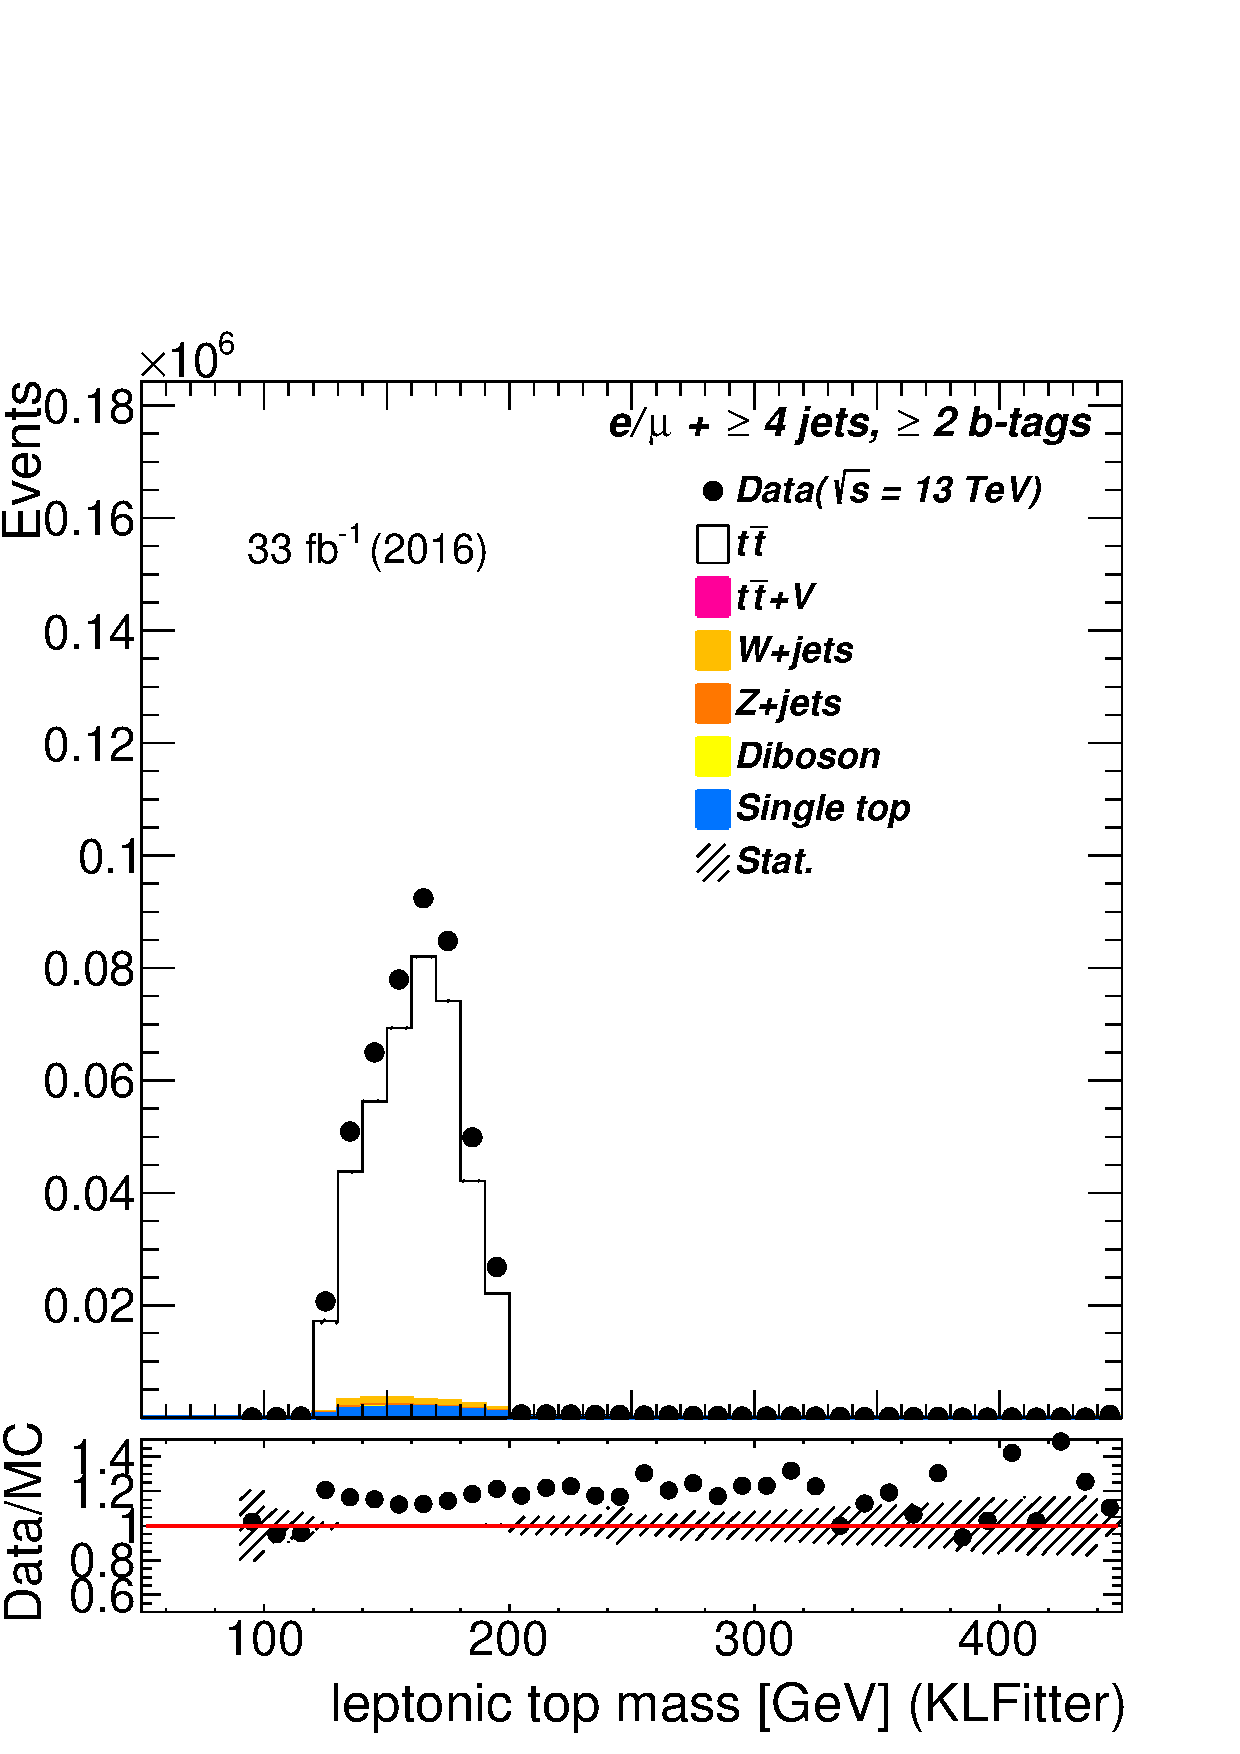
\includegraphics[width=\linewidth]{ControlPlots_emujets_2016_4incl_2incl/klf_topLep_m_emujets_2016.png}
		\caption{ Invariant mass of the leptonic top quark.} \label{fig:K16}
	\end{subfigure}\hspace*{0.25cm}
	\begin{subfigure}{0.25\textwidth}
		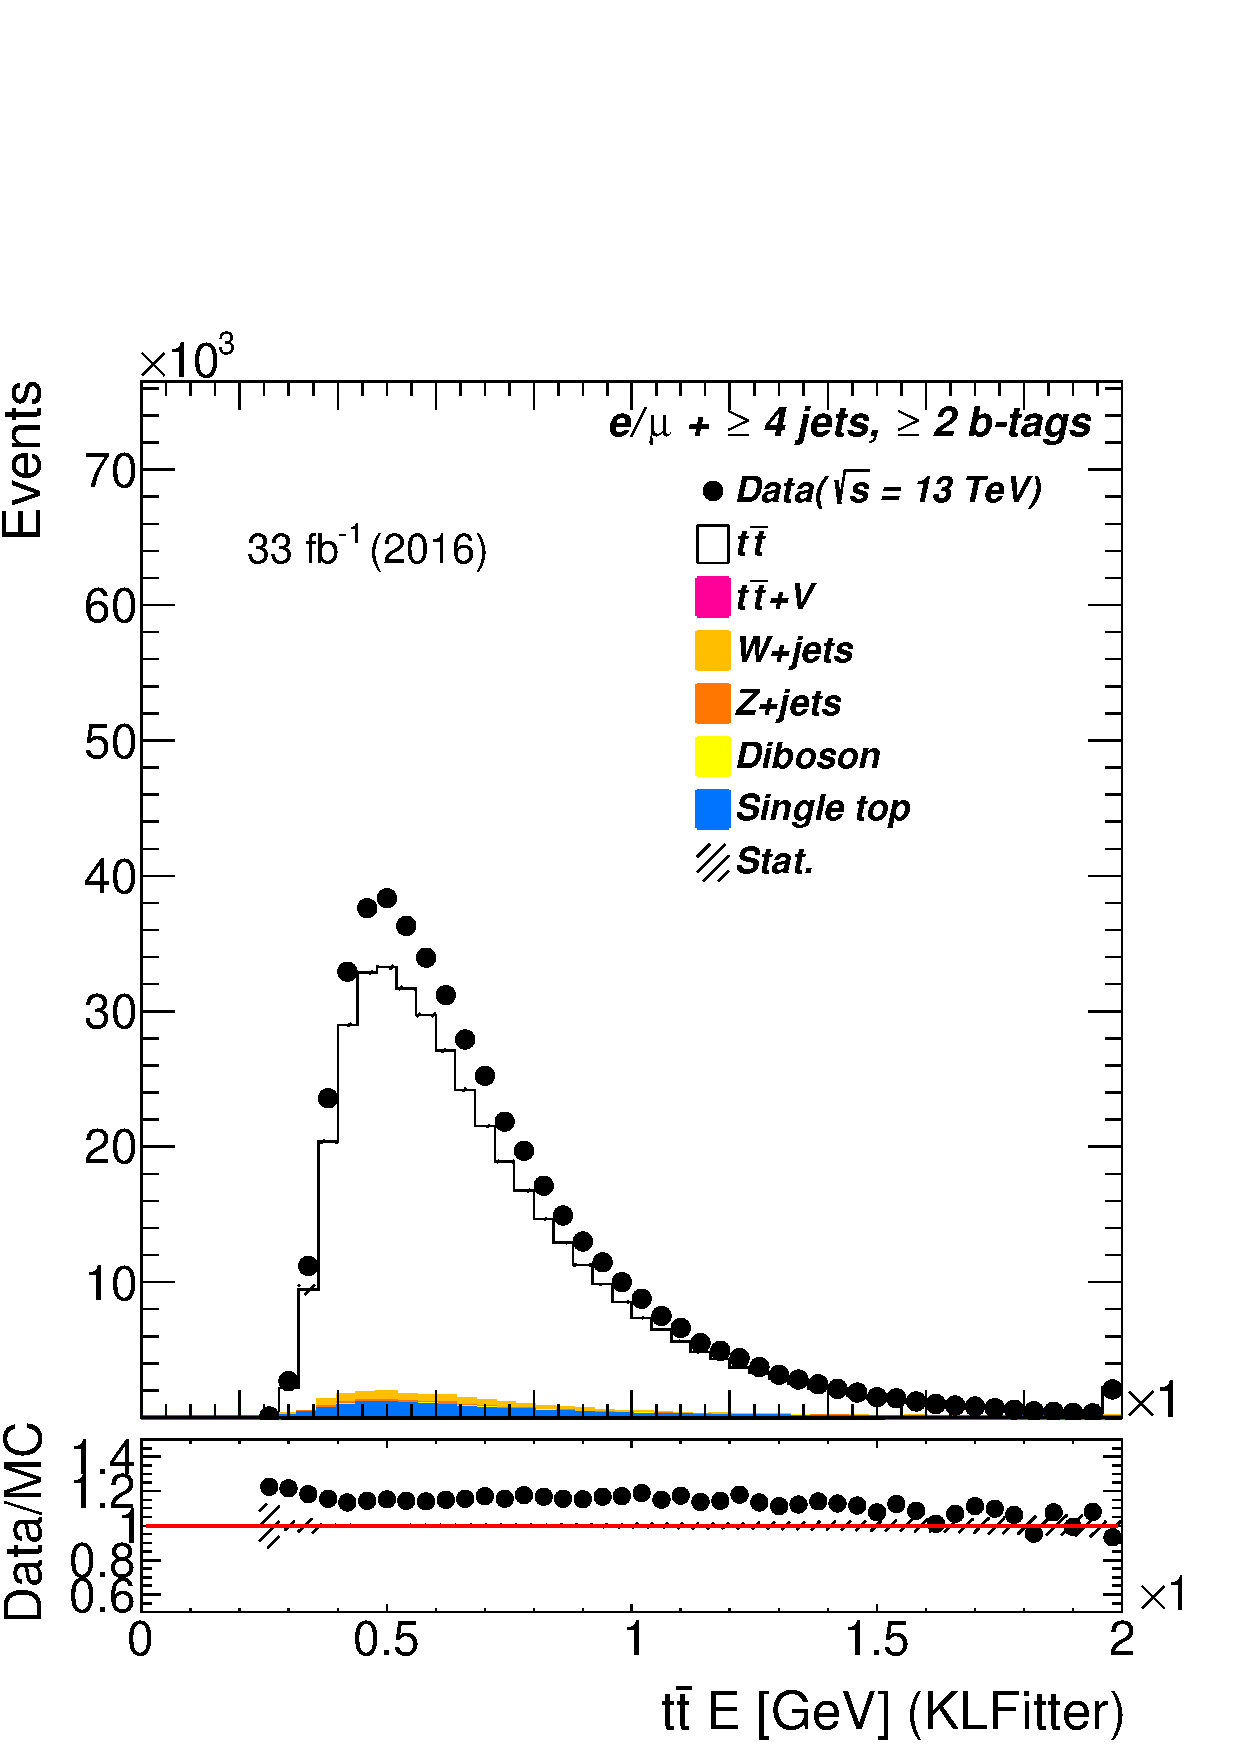
\includegraphics[width=\linewidth]{ControlPlots_emujets_2016_4incl_2incl/klf_ttbar_E_emujets_2016.png}
		\caption{Energy of the top-quark pair.} \label{fig:K17}
	\end{subfigure}


	\begin{subfigure}{0.25\textwidth}
		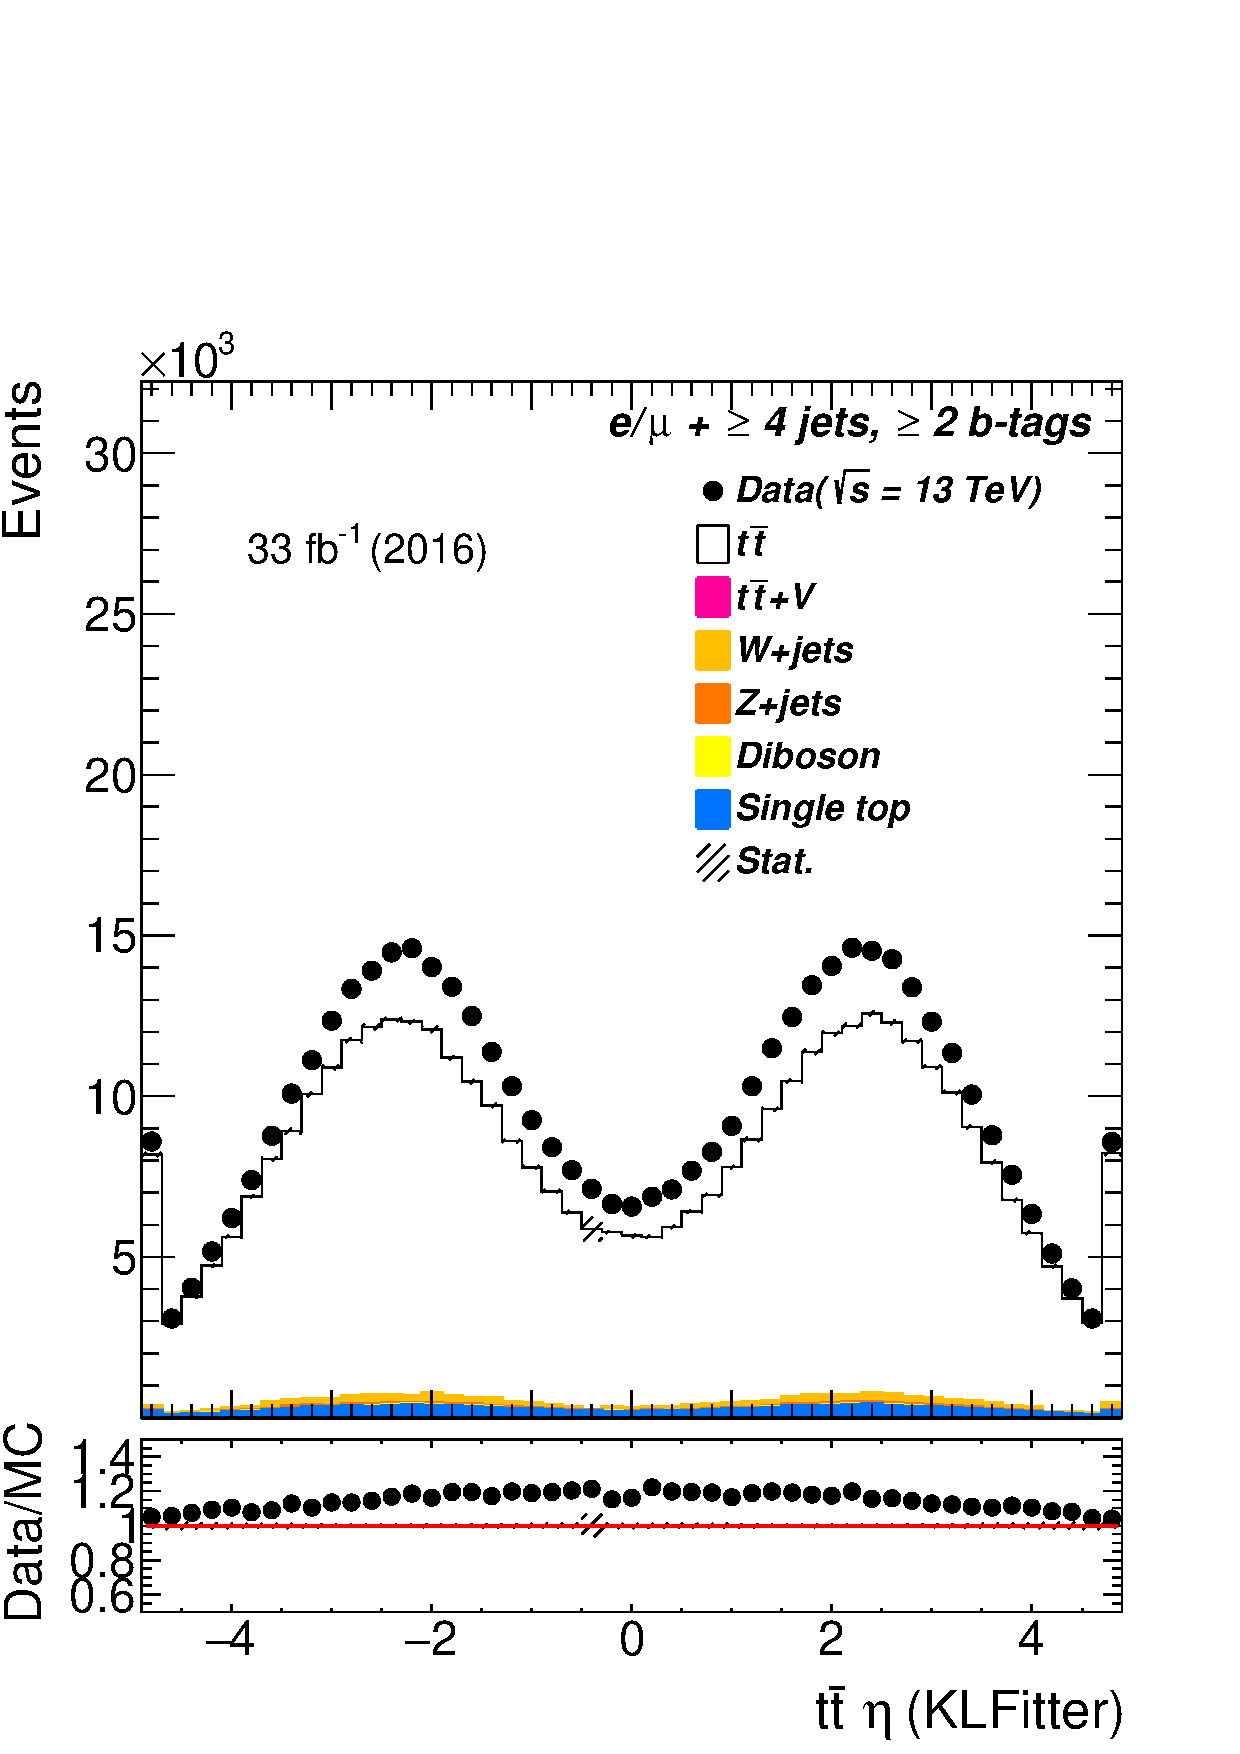
\includegraphics[width=\linewidth]{ControlPlots_emujets_2016_4incl_2incl/klf_ttbar_eta_emujets_2016.png}
		\caption{Rapidity of the top-quark pair.} \label{fig:K18}
	\end{subfigure}
	\hspace*{0.5cm}
	\begin{subfigure}{0.25\textwidth}
		\includegraphics[width=\linewidth]{ControlPlots_emujets_2016_4incl_2incl/klf_ttbar_phi_emujets_2016.png}
		\caption{$\phi$  distribution of the top-quark pair.                       } \label{fig:K19}
	\end{subfigure}
\hspace*{0.5cm}
	\begin{subfigure}{0.25\textwidth}
		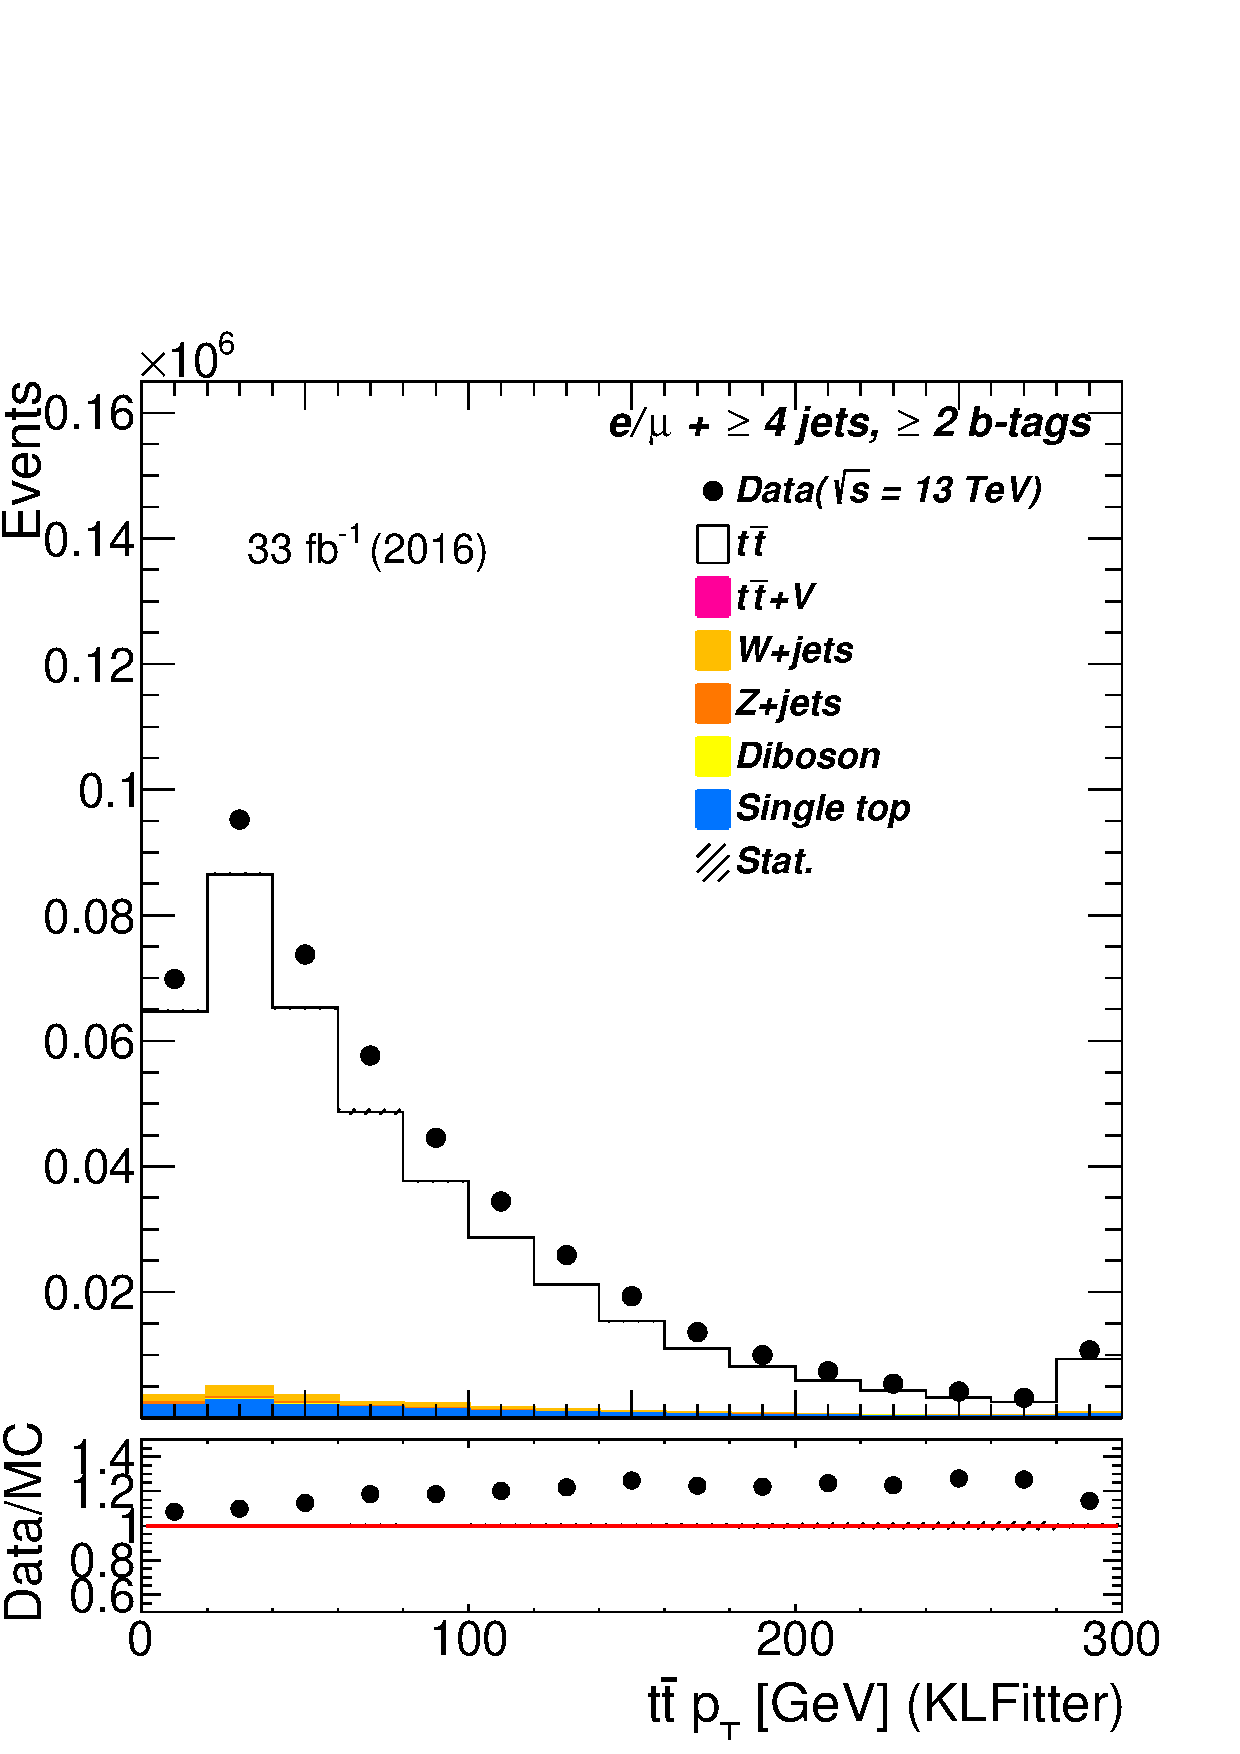
\includegraphics[width=\linewidth]{ControlPlots_emujets_2016_4incl_2incl/klf_ttbar_pt_emujets_2016.png}
		\caption{Transverse momentum of the top-quark pair.} \label{fig:K20}
	\end{subfigure}
	
	\caption{Same plots as for~\cref{klf100} of the  global properties of the leptonic and hadronic top-quark, as well as of the top-quark pair, reconstructed with \textsc{KLFitter}.  }
\end{figure}	













